%
% Draft  document skinwool.tex
% Notes on genetic analysis of ab32 and ab20 skin and wool data
%
 
\documentclass[titlepage]{article}  % Latex2e
\usepackage{graphicx,lscape,subfigure}
\usepackage{bm,longtable}
\usepackage{textcomp}
 

\title{ Genetic relationship between skin and wool traits in Merino sheep}
\author{Neville Jackson }
\date{27 Oct 2015} 

 
\begin{document} 
 
\maketitle      
\tableofcontents

\clearpage
\section{Acknowledgement}
The data analysed here were collected while I worked at CSIRO Division of Animal Genetics and Division of Animal Production. I would like to acknowledge the contributions of Dr Ted Nay and Mr Ian Maddocks, and the encouragement given by Dr Helen Newton Turner, Dr J M Rendel, Dr A A Dunlop, and Dr T W Scott. I would also like to acknowledge the encouragement of Dr J M Watts in resurrecting this material for re-analysis with more advanced statistical technology, and in suggesting that the emphasis should be on fibre characteristics related to processing performance and procduct quality as well as production characteristics such as clean wool weight.


\clearpage
\section{Abstract}

\clearpage
\section{Introduction} 
	Some years ago an attempt was made to study the relationship between components of clean wool weight and skin characteristics obtained from histological examination of skin biopsy samples (Jackson, Nay, and Turner(1975)~\cite{jack:75}. What came out of that study was that skin characteristics could explain a large proportion of the genetic variatrion in clean wool weight, and that the genetic covariance between skin characteristics and wool weight components could be partitioned into three independent functional relationships which were interpreted as three independent sets of genes.

	The three independent factors were identified as 
\begin{itemize}
\item large number of secondary follicles
\item straight deep follicles
\item primary follicle density
\end{itemize}

	This analysis led to a selection experiment (AB32 in CSIRO jargon) which attempted to select for
\begin{itemize}
\item large follicles
\item large total number of follicles
\item both large follicles and large number of follicles simultaneously
\end{itemize}
in three selected lines. There was also an unselected control line.

During the course of that experiment some image analysis technology was developed for skin section images. This allowed measurement of the diameter of primary and secondary follicles, in addition to counting their density. These new measurements are available only on the last three years of the experiment but are an important extension which may change the scope and focus of the above multivriate analyses.

There has also been some important progress in our understanding of follicle development in sheep. The work of Moore(....) has shown that follicles develop from a population of pre-papilla cells and that if primary follicle development is suppressed (fewer or smaller primaries) then there are more pre-papilla cells left over to divide, and to develop into secondary follicles. The dynamics of the pre-papilla cell population can be modelled mathematically, so that the relationship between primary development and secondary development can be quantified. The consequences of this for a genetic analysis of primary and secondary follicle development are significant - there is nonlinearity and an element of functional relationships between traits neither of which are taken into account in traditional quantitative genetic analyses.

The objectives of this study  are diverse and probably overambitious. Briefly we would like to
\begin{itemize}
\item summarize the response to selection which was obtained in the above experiment
\item estimate additive genetic parameters for a comprehensive range of skin and wool characteristics
\item redo the multivariate analyses mentioned above with an emphasis on fibre quality as well as wool production
\item work out how to include knowledge of the developmental relationships between characteristics in a quantitative genetic analysis and apply this to the Moore model mentioned above
\item do a systematic check for nonlinearities and shifts in genetic parameters, and find a way of including these in a quantitative genetic analysis
\end{itemize}
One of the benefits of setting out such a broad objective is that the areas where we fail become indicators of future research directions.

\section{Materials and methods}
The sheep and the measurements thereon included in this study represent a substantial investment of CSIRO resources over 11 years of a breeding trial and several more years of laboratory measurement work. Unfortunately the experiment was terminated abruptly by a political decision and was never properly analysed or published. What we have, for the present study, is a set of measurements exhibiting various degrees of incompleteness. The present analysis is therefore somewhat complicated and the results may be affected by the severe imbalance with respect to some traits.

\subsection{ Sheep population studied}
The selection experiment is known as AB32 in CSIRO jargon. It commenced in 1974. For two years (1974 and 1975) matings were made of a set of introduced Fine Merino rams across a set of CSIRO bred Medium Merino ewes to generate the base generation animals for a selection trial. Measurements were made on these base generation progeny.

Then, starting with the 1976 mating, the base generation animals were allocate at random to three selection lines and then selected as follows
\begin{description}
\item[Line 1] selected for large follicle depth
\item[Line 2] selected for large number of follicles per head (estimated by multiplying follicle density by body surface area)
\item[Line 3] selected for both large follicle depth and large number of follicles per head
\end{description}
Selection continued until 1985, the animals born in 1985 being the last progeny of the selected lines with measurements available.

There was also an unselected control line ( AB20 in CSIRO jargon) which was a group of Medium Merino sheep which served as an unselected control for all sheep selection experimants at 'Longford' Research Station. The control line structure is described in Watson, Jackson, and Whiteley(1977)~\cite{wats:77}.

Pedigree information was available on all sheep, in the case of AB32 extending back to 1974, and in the case of AB20 extendoing back to 1968.

\subsection{Traits measured}
There were several categories of traits considered for analysis. 

\subsubsection{Traits for which direct measurements were available}
A brief description of the traits for which measurements were available is given in Table~\ref{tab:tdef}.

%\documentclass{article}
%\usepackage{lscape,longtable}
%\begin{document}
\begin{center}
\begin{landscape}
\begin{longtable}{p{1.5in}|p{0.8in}|p{1.5in}|p{1.0in}|p{2.5in}}
\caption{Definition of traits measured}  \\
\hline
\label{tab:tdef}
    Trait name & Abbreviation  & Units & Age measured  &  Description \\ 
\hline
\endfirsthead
\multicolumn{5}{c}%
{\tablename\ \thetable\ -- \textit{Continued from previous page}} \\
\hline
    Trait name & Abbreviation  & Units & Age measured  &  Description \\ 
\hline
\endhead
\hline
\multicolumn{5}{r}{\textit{Continued on next page}} \\
\endfoot
\hline
\endlastfoot
%\env{longtable}[p{1.5in}|p{0.8in}|p{1.5in}|p{1.0in}|p{2.5in}]
 Staple length & Stal & mm & 14 months & Length of wool staple 10 months growth \\
 Crimp frequency & Crimp & no per 2.5cm & 14 months & Staple crimp frequency\\
 Fibre diameter & Diam & microns & 14 months & Mean fibre diameter by airflow technique \\
 Greasy Fleece Weight & Gfw & Kg & 14 months & Weight of fleece in shearing shed \\
 Yield & Yld & percentage & 14 months & Percent of clean wool in fleece at 16\% regain \\
 Clean wool weight & Cww & Kg & 14 months & Weight of clean fibre at 16\% regain \\
 Bodyweight & Bwt & Kg & 14 months & Live weight of animal \\
 Neck wrinkle & WrN & score 0-6 (0=plain,6=wrinkled) & 14 months & Score for skin wrinkle on neck region \\
 Body wrinkle & WrB & score 0-5 (0=plain,5=wrinkled) & 14 months & Score for skin wrinkle on body region \\
 Total wrinkle & WrT & sum of WrN and WrB & 14 months & Sum of neck and body wrinkle scores \\
 Face cover & Face & score 1-7 (1=open, 7=muffled) & 14 months & Score for wool cover on the face \\
 Adjusted staple length & Staladj & mm per 365 days & 14 months & Staple length adjusted to a growth period of 365 days \\
 Adjusted clean wool weight & Cwwadj & Kg per 365 days & 14 months & Clean wool weight adjusted to a growth period of 365 days \\
 Adjusted greasy fleece weight & Gfwadj & Kg per 365 days & 14 months & Greasy fleece weight adjusted to a growth period of 365 days \\
 Follicle number per unit area & Fnua & no per $mm_{2}$ & 14 months & No of primary and secondary follicles per $mm_{2}$ from skin biopsy \\
 Follicle $S/P$ ratio & Fr & no units & 14 months & Ratio of no of primary to no of secondary follicles from skin biopsy \\
 Total follicle number & Fnt & no per head x $10^{6}$ & 14 months & No of follicles on the animal (estimated from Fnua and skin surface area) \\
  Surface area & Sarea & $m^{2}$ & 14 months & Smooth skin surface area (estimated from Bwt with no allowance for wrinkle) \\
  Follicle depth & Fd & mm & 14 months & Average follicle depth from skin biopsy and vertical section \\
  Follicle curvature & Fc & score 1-7 (1=straight, 7=curved) & 14 months & Follicle curvature score from skin biopsy and vertical section \\
  Follicle unevenness & Fu & score 1-5 (1=even, 5=uneven) & 14 months & Score for unevenness of follicle depth from skin biopsy and vertical section \\
  Birth weight & Birwt & Kg & day of birth & Weight of lamb on day of birth \\
  Birthcoat score side & Bcts & score 1-6 (1=no halo hairs on side, 6=fully covered) & day of birth & Score for pattern of halo hairs on side of lamb at day of birth \\
  Birthcoat score back & Bctb & score 1-6 (1=no halo hairs on mid backline, 6=dense halo hairs) & day of birth & Score for density of halo hairs on mid backline on day of birth \\
  Weaning weight & Weanwt & Kg & approx 4 months & Weight of lamb on day of weaning \\
  Weaner greasy fleece weight & WeanGfw & Kg & approx 4 months &  Weaner greasy fleece weight at post-weaning shearing \\
  No of lambs born & NLB & no & day of birth & Number of lambs in litter at birth \\
  No of lambs weaned & NLW & no & approx 4 months & Number of lambs in litter at weaning \\
 Greasy wool colour & Colour & score 1-7 (1=white, 7=yellow) & 14 months & Score for greasy yolk colour ignoring any stain present \\
 Flystrike & Fly & score 0-9 (0=absent, 1-9=present to various degrees) & 14 months & Score for presence or absene of flystrike at any site \\
 Fleece rot & Flcrot & score 0-9 (0=absent, 1-9=present to various degrees) & 14 months & Score for presence or absence of fleece rot \\
 Bacterial stain & Bactst & score 0-9 (0=absent, 1-9=present to various degrees) & 14 months & Score for presence or absence of bacterial stain \\
 Mycotic dermatitis & MycD & score 0-9 (0=absent, 1-9=present to various degrees) & 14 months & Score for presence or absence of mycotic dermatitis \\
  Mean diameter of primaries & Dp & microns & 14 months & Mean diameter of primary fibres from biopsy and horizontal section \\
  Mean diameter of secondaries & Ds & microns & 14 months & Mean diameter of secondary fibres from biopsy and horizontal section \\
  Mean diameter of primaries and secondaries & Dps & microns & 14 months & Mean diameter of primary and secondary fibres from biopsy and horizontal section \\
  Primary to secondary diameter ratio & DpovDs & no units & 14 months & Ratio of mean diameter of primary fibres to mean diameter of secondary fibres \\
  CV of primary diameter & CVDp & no units & 14 months & Coefficient of variation of primary fibre diameter \\
  CV of secondary diameter & CVDs & no units & 14 months & Coefficient of variation of secondary fibre diameter \\
  Maximum diameter of primaries & MaxDp & microns & 14 months & Diameter of the largest primary fibre \\
  Minimum diameter of primaries & MinDp & microns & 14 months & Diameter of the smallest primary fibre \\
  Maximum diameter of secondaries & MaxDs & microns & 14 months & Diameter of the largest secondary fibre \\
  Minimum diameter of secondaries & MinDs & microns & 14 months & Diameter of the smallest secondary fibre \\
  SD of primaries & SDDp & microns & 14 months & Standard deviation of primary fibre diameter \\
  SD of secondaries & SDDs & microns & 14 months & Standard deviation of secondary fibre diameter \\
  SD of all fibres & SDD & microns & 14 months & Standard deviation of primary and secondary fibre diameter \\
  CV of all fibres & CVD & no units & 14 months & Coefficient of variation of primary and secondary fibre diameter \\
  Primaries greater than 30 microns & Gt30Dp & frequency & 14 months & Proportion of primary fibres exceeding 30 microns in diameter \\
  Secondaries greater than 30 microns & Gt30Ds & frequency & 14 months & Proportion of secondary fibres exceeding 30 microns in diameter \\
  Fibres greater than 30 microns & Gt30D & frequency & 14 months & Proportion of fibres exceeding 30 microns in diameter \\

\end{longtable}
\end{landscape}
\end{center}
%\end{document}


All of these measured traits were not available on all of the sheep. In particular the traits obtained by image analysis measurement on skin sections were only obtained for the 1982 to 1985 drops of selected lines and only the 1983 and 1985 drops of the control line. Also Crimp Frequency was only measured for 1974 to 1977 and 1982 to 1985. Various other subsets of traits had various patterns of missing observations. 

The actual numbers of sheep measured for each trait and each pair of traits is given in Tables~\ref{tab:counts1} to ~\ref{tab:counts5}. It can be seen that each pair of traits has a different number of observations, with the exception that there are some subsets of traits ( such as the 17 image analysis traits from Dp to Gt30D) for which the replication almost identical. Two traits, Birwt and WeanGfw, had very few observations when paired with the image analysis traits (Dp, etc) and had to be omitted from most of the analyses.

% latex table generated in R 3.2.2 by xtable 1.8-0 package
% Thu Nov 19 20:37:14 2015
\begin{table}[p]
\footnotesize
\centering
\caption{Numbers of sheep measured for each pair of traits: Part 1/5.} 
\label{tab:counts1}
\begin{tabular}{rrrrrrrrrrr}
  \hline
 & Stal & Crimp & Diam & Gfw & Yld & Cww & Bwt & WrN & WrB & WrT \\ 
  \hline
Stal & 3651 & 2227 & 3632 & 3638 & 3632 & 3632 & 3622 & 3619 & 3616 & 3616 \\ 
  Crimp & 2227 & 2227 & 2213 & 2218 & 2213 & 2213 & 2205 & 2202 & 2199 & 2199 \\ 
  Diam & 3632 & 2213 & 3638 & 3637 & 3637 & 3637 & 3620 & 3617 & 3614 & 3614 \\ 
  Gfw & 3638 & 2218 & 3637 & 3643 & 3637 & 3637 & 3624 & 3621 & 3618 & 3618 \\ 
  Yld & 3632 & 2213 & 3637 & 3637 & 3637 & 3637 & 3619 & 3616 & 3613 & 3613 \\ 
  Cww & 3632 & 2213 & 3637 & 3637 & 3637 & 3637 & 3619 & 3616 & 3613 & 3613 \\ 
  Bwt & 3622 & 2205 & 3620 & 3624 & 3619 & 3619 & 3629 & 3625 & 3622 & 3622 \\ 
  WrN & 3619 & 2202 & 3617 & 3621 & 3616 & 3616 & 3625 & 3626 & 3623 & 3623 \\ 
  WrB & 3616 & 2199 & 3614 & 3618 & 3613 & 3613 & 3622 & 3623 & 3623 & 3623 \\ 
  WrT & 3616 & 2199 & 3614 & 3618 & 3613 & 3613 & 3622 & 3623 & 3623 & 3623 \\ 
  Face & 3644 & 2220 & 3630 & 3635 & 3629 & 3629 & 3620 & 3617 & 3614 & 3614 \\ 
  Staladj & 3572 & 2157 & 3553 & 3559 & 3553 & 3553 & 3543 & 3540 & 3538 & 3538 \\ 
  Cwwadj & 3553 & 2143 & 3558 & 3558 & 3558 & 3558 & 3540 & 3537 & 3535 & 3535 \\ 
  Gfwadj & 3559 & 2148 & 3558 & 3564 & 3558 & 3558 & 3545 & 3542 & 3540 & 3540 \\ 
  Fnua & 3092 & 1768 & 3084 & 3087 & 3083 & 3083 & 3078 & 3076 & 3073 & 3073 \\ 
  Fr & 3093 & 1768 & 3085 & 3088 & 3084 & 3084 & 3079 & 3077 & 3074 & 3074 \\ 
  Fnt & 3074 & 1751 & 3075 & 3077 & 3074 & 3074 & 3079 & 3076 & 3073 & 3073 \\ 
  Sarea & 3074 & 1752 & 3074 & 3077 & 3073 & 3073 & 3078 & 3075 & 3072 & 3072 \\ 
  Fd & 2587 & 1281 & 2580 & 2582 & 2579 & 2579 & 2575 & 2573 & 2570 & 2570 \\ 
  Fc & 2587 & 1281 & 2580 & 2582 & 2579 & 2579 & 2575 & 2573 & 2570 & 2570 \\ 
  Fu & 2587 & 1281 & 2580 & 2582 & 2579 & 2579 & 2575 & 2573 & 2570 & 2570 \\ 
  Birwt & 925 & 645 & 924 & 925 & 923 & 923 & 919 & 918 & 918 & 918 \\ 
  Bcts & 3641 & 2219 & 3628 & 3633 & 3627 & 3627 & 3619 & 3616 & 3613 & 3613 \\ 
  Bctb & 3161 & 1739 & 3148 & 3151 & 3147 & 3147 & 3139 & 3137 & 3134 & 3134 \\ 
  Weanwt & 3646 & 2223 & 3633 & 3638 & 3632 & 3632 & 3624 & 3621 & 3618 & 3618 \\ 
  WeanGfw & 1679 & 1015 & 1679 & 1681 & 1679 & 1679 & 1674 & 1671 & 1668 & 1668 \\ 
  NLB & 3645 & 2221 & 3632 & 3637 & 3631 & 3631 & 3623 & 3620 & 3618 & 3618 \\ 
  NLW & 3645 & 2221 & 3632 & 3637 & 3631 & 3631 & 3623 & 3620 & 3618 & 3618 \\ 
  Dp & 825 & 468 & 823 & 824 & 823 & 823 & 821 & 821 & 821 & 821 \\ 
  Ds & 825 & 468 & 823 & 824 & 823 & 823 & 821 & 821 & 821 & 821 \\ 
  Dps & 825 & 468 & 823 & 824 & 823 & 823 & 821 & 821 & 821 & 821 \\ 
  DpovDs & 825 & 468 & 823 & 824 & 823 & 823 & 821 & 821 & 821 & 821 \\ 
  CVDp & 825 & 468 & 823 & 824 & 823 & 823 & 821 & 821 & 821 & 821 \\ 
  CVDs & 825 & 468 & 823 & 824 & 823 & 823 & 821 & 821 & 821 & 821 \\ 
  MaxDp & 825 & 468 & 823 & 824 & 823 & 823 & 821 & 821 & 821 & 821 \\ 
  MinDp & 825 & 468 & 823 & 824 & 823 & 823 & 821 & 821 & 821 & 821 \\ 
  MaxDs & 825 & 468 & 823 & 824 & 823 & 823 & 821 & 821 & 821 & 821 \\ 
  MinDs & 825 & 468 & 823 & 824 & 823 & 823 & 821 & 821 & 821 & 821 \\ 
  SDDp & 825 & 468 & 823 & 824 & 823 & 823 & 821 & 821 & 821 & 821 \\ 
  SDDs & 825 & 468 & 823 & 824 & 823 & 823 & 821 & 821 & 821 & 821 \\ 
  SDD & 825 & 468 & 823 & 824 & 823 & 823 & 821 & 821 & 821 & 821 \\ 
  CVD & 825 & 468 & 823 & 824 & 823 & 823 & 821 & 821 & 821 & 821 \\ 
  Gt30Dp & 825 & 468 & 823 & 824 & 823 & 823 & 821 & 821 & 821 & 821 \\ 
  Gt30Ds & 825 & 468 & 823 & 824 & 823 & 823 & 821 & 821 & 821 & 821 \\ 
  Gt30D & 825 & 468 & 823 & 824 & 823 & 823 & 821 & 821 & 821 & 821 \\ 
  Colour & 3393 & 1971 & 3388 & 3391 & 3387 & 3387 & 3377 & 3375 & 3375 & 3375 \\ 
  Fly & 3396 & 1972 & 3391 & 3394 & 3390 & 3390 & 3380 & 3378 & 3378 & 3378 \\ 
  Flcrot & 3396 & 1972 & 3391 & 3394 & 3390 & 3390 & 3380 & 3378 & 3378 & 3378 \\ 
  Bactst & 2279 & 855 & 2270 & 2273 & 2269 & 2269 & 2271 & 2270 & 2270 & 2270 \\ 
  MycD & 2279 & 855 & 2270 & 2273 & 2269 & 2269 & 2271 & 2270 & 2270 & 2270 \\ 
   \hline
\end{tabular}
\normalsize
\end{table}

% latex table generated in R 3.2.2 by xtable 1.8-0 package
% Thu Nov 19 20:47:25 2015
\begin{table}[p]
\footnotesize
\centering
\caption{Numbers of sheep measured for each pair of traits: Part 2/5.} 
\label{tab:counts2}
\begin{tabular}{rrrrrrrrrrr}
  \hline
 & Face & Staladj & Cwwadj & Gfwadj & Fnua & Fr & Fnt & Sarea & Fd & Fc \\ 
  \hline
Stal & 3644 & 3572 & 3553 & 3559 & 3092 & 3093 & 3074 & 3074 & 2587 & 2587 \\ 
  Crimp & 2220 & 2157 & 2143 & 2148 & 1768 & 1768 & 1751 & 1752 & 1281 & 1281 \\ 
  Diam & 3630 & 3553 & 3558 & 3558 & 3084 & 3085 & 3075 & 3074 & 2580 & 2580 \\ 
  Gfw & 3635 & 3559 & 3558 & 3564 & 3087 & 3088 & 3077 & 3077 & 2582 & 2582 \\ 
  Yld & 3629 & 3553 & 3558 & 3558 & 3083 & 3084 & 3074 & 3073 & 2579 & 2579 \\ 
  Cww & 3629 & 3553 & 3558 & 3558 & 3083 & 3084 & 3074 & 3073 & 2579 & 2579 \\ 
  Bwt & 3620 & 3543 & 3540 & 3545 & 3078 & 3079 & 3079 & 3078 & 2575 & 2575 \\ 
  WrN & 3617 & 3540 & 3537 & 3542 & 3076 & 3077 & 3076 & 3075 & 2573 & 2573 \\ 
  WrB & 3614 & 3538 & 3535 & 3540 & 3073 & 3074 & 3073 & 3072 & 2570 & 2570 \\ 
  WrT & 3614 & 3538 & 3535 & 3540 & 3073 & 3074 & 3073 & 3072 & 2570 & 2570 \\ 
  Face & 3649 & 3565 & 3550 & 3556 & 3092 & 3093 & 3074 & 3074 & 2587 & 2587 \\ 
  Staladj & 3565 & 3572 & 3553 & 3559 & 3043 & 3044 & 3025 & 3025 & 2567 & 2567 \\ 
  Cwwadj & 3550 & 3553 & 3558 & 3558 & 3034 & 3035 & 3025 & 3024 & 2559 & 2559 \\ 
  Gfwadj & 3556 & 3559 & 3558 & 3564 & 3038 & 3039 & 3028 & 3028 & 2562 & 2562 \\ 
  Fnua & 3092 & 3043 & 3034 & 3038 & 3097 & 3097 & 3078 & 3079 & 2590 & 2590 \\ 
  Fr & 3093 & 3044 & 3035 & 3039 & 3097 & 3098 & 3079 & 3079 & 2591 & 2591 \\ 
  Fnt & 3074 & 3025 & 3025 & 3028 & 3078 & 3079 & 3079 & 3078 & 2574 & 2574 \\ 
  Sarea & 3074 & 3025 & 3024 & 3028 & 3079 & 3079 & 3078 & 3079 & 2573 & 2573 \\ 
  Fd & 2587 & 2567 & 2559 & 2562 & 2590 & 2591 & 2574 & 2573 & 2592 & 2592 \\ 
  Fc & 2587 & 2567 & 2559 & 2562 & 2590 & 2591 & 2574 & 2573 & 2592 & 2592 \\ 
  Fu & 2587 & 2567 & 2559 & 2562 & 2590 & 2591 & 2574 & 2573 & 2592 & 2592 \\ 
  Birwt & 925 & 899 & 897 & 899 & 580 & 580 & 579 & 579 & 484 & 484 \\ 
  Bcts & 3639 & 3562 & 3548 & 3554 & 3090 & 3091 & 3072 & 3072 & 2585 & 2585 \\ 
  Bctb & 3163 & 3088 & 3074 & 3078 & 2670 & 2671 & 2655 & 2655 & 2164 & 2164 \\ 
  Weanwt & 3644 & 3567 & 3553 & 3559 & 3095 & 3096 & 3077 & 3077 & 2590 & 2590 \\ 
  WeanGfw & 1676 & 1656 & 1656 & 1658 & 1476 & 1476 & 1473 & 1473 & 1428 & 1428 \\ 
  NLB & 3643 & 3572 & 3558 & 3564 & 3091 & 3092 & 3073 & 3073 & 2588 & 2588 \\ 
  NLW & 3643 & 3572 & 3558 & 3564 & 3091 & 3092 & 3073 & 3073 & 2588 & 2588 \\ 
  Dp & 825 & 798 & 796 & 797 & 824 & 825 & 821 & 821 & 338 & 338 \\ 
  Ds & 825 & 798 & 796 & 797 & 824 & 825 & 821 & 821 & 338 & 338 \\ 
  Dps & 825 & 798 & 796 & 797 & 824 & 825 & 821 & 821 & 338 & 338 \\ 
  DpovDs & 825 & 798 & 796 & 797 & 824 & 825 & 821 & 821 & 338 & 338 \\ 
  CVDp & 825 & 798 & 796 & 797 & 824 & 825 & 821 & 821 & 338 & 338 \\ 
  CVDs & 825 & 798 & 796 & 797 & 824 & 825 & 821 & 821 & 338 & 338 \\ 
  MaxDp & 825 & 798 & 796 & 797 & 824 & 825 & 821 & 821 & 338 & 338 \\ 
  MinDp & 825 & 798 & 796 & 797 & 824 & 825 & 821 & 821 & 338 & 338 \\ 
  MaxDs & 825 & 798 & 796 & 797 & 824 & 825 & 821 & 821 & 338 & 338 \\ 
  MinDs & 825 & 798 & 796 & 797 & 824 & 825 & 821 & 821 & 338 & 338 \\ 
  SDDp & 825 & 798 & 796 & 797 & 824 & 825 & 821 & 821 & 338 & 338 \\ 
  SDDs & 825 & 798 & 796 & 797 & 824 & 825 & 821 & 821 & 338 & 338 \\ 
  SDD & 825 & 798 & 796 & 797 & 824 & 825 & 821 & 821 & 338 & 338 \\ 
  CVD & 825 & 798 & 796 & 797 & 824 & 825 & 821 & 821 & 338 & 338 \\ 
  Gt30Dp & 825 & 798 & 796 & 797 & 824 & 825 & 821 & 821 & 338 & 338 \\ 
  Gt30Ds & 825 & 798 & 796 & 797 & 824 & 825 & 821 & 821 & 338 & 338 \\ 
  Gt30D & 825 & 798 & 796 & 797 & 824 & 825 & 821 & 821 & 338 & 338 \\ 
  Colour & 3390 & 3320 & 3314 & 3318 & 2844 & 2845 & 2833 & 2833 & 2339 & 2339 \\ 
  Fly & 3393 & 3320 & 3314 & 3318 & 2845 & 2846 & 2834 & 2834 & 2340 & 2340 \\ 
  Flcrot & 3393 & 3320 & 3314 & 3318 & 2845 & 2846 & 2834 & 2834 & 2340 & 2340 \\ 
  Bactst & 2280 & 2214 & 2204 & 2208 & 1812 & 1813 & 1809 & 1809 & 1307 & 1307 \\ 
  MycD & 2280 & 2214 & 2204 & 2208 & 1812 & 1813 & 1809 & 1809 & 1307 & 1307 \\ 
   \hline
\end{tabular}
\normalsize
\end{table}

% latex table generated in R 3.2.2 by xtable 1.8-0 package
% Thu Nov 19 20:51:15 2015
\begin{table}[p]
\footnotesize
\centering
\caption{Numbers of sheep measured for each pair of traits: Part 3/5.} 
\label{tab:counts3}
\begin{tabular}{rrrrrrrrrrr}
  \hline
 & Fu & Birwt & Bcts & Bctb & Weanwt & WeanGfw & NLB & NLW & Dp & Ds \\ 
  \hline
Stal & 2587 & 925 & 3641 & 3161 & 3646 & 1679 & 3645 & 3645 & 825 & 825 \\ 
  Crimp & 1281 & 645 & 2219 & 1739 & 2223 & 1015 & 2221 & 2221 & 468 & 468 \\ 
  Diam & 2580 & 924 & 3628 & 3148 & 3633 & 1679 & 3632 & 3632 & 823 & 823 \\ 
  Gfw & 2582 & 925 & 3633 & 3151 & 3638 & 1681 & 3637 & 3637 & 824 & 824 \\ 
  Yld & 2579 & 923 & 3627 & 3147 & 3632 & 1679 & 3631 & 3631 & 823 & 823 \\ 
  Cww & 2579 & 923 & 3627 & 3147 & 3632 & 1679 & 3631 & 3631 & 823 & 823 \\ 
  Bwt & 2575 & 919 & 3619 & 3139 & 3624 & 1674 & 3623 & 3623 & 821 & 821 \\ 
  WrN & 2573 & 918 & 3616 & 3137 & 3621 & 1671 & 3620 & 3620 & 821 & 821 \\ 
  WrB & 2570 & 918 & 3613 & 3134 & 3618 & 1668 & 3618 & 3618 & 821 & 821 \\ 
  WrT & 2570 & 918 & 3613 & 3134 & 3618 & 1668 & 3618 & 3618 & 821 & 821 \\ 
  Face & 2587 & 925 & 3639 & 3163 & 3644 & 1676 & 3643 & 3643 & 825 & 825 \\ 
  Staladj & 2567 & 899 & 3562 & 3088 & 3567 & 1656 & 3572 & 3572 & 798 & 798 \\ 
  Cwwadj & 2559 & 897 & 3548 & 3074 & 3553 & 1656 & 3558 & 3558 & 796 & 796 \\ 
  Gfwadj & 2562 & 899 & 3554 & 3078 & 3559 & 1658 & 3564 & 3564 & 797 & 797 \\ 
  Fnua & 2590 & 580 & 3090 & 2670 & 3095 & 1476 & 3091 & 3091 & 824 & 824 \\ 
  Fr & 2591 & 580 & 3091 & 2671 & 3096 & 1476 & 3092 & 3092 & 825 & 825 \\ 
  Fnt & 2574 & 579 & 3072 & 2655 & 3077 & 1473 & 3073 & 3073 & 821 & 821 \\ 
  Sarea & 2573 & 579 & 3072 & 2655 & 3077 & 1473 & 3073 & 3073 & 821 & 821 \\ 
  Fd & 2592 & 484 & 2585 & 2164 & 2590 & 1428 & 2588 & 2588 & 338 & 338 \\ 
  Fc & 2592 & 484 & 2585 & 2164 & 2590 & 1428 & 2588 & 2588 & 338 & 338 \\ 
  Fu & 2592 & 484 & 2585 & 2164 & 2590 & 1428 & 2588 & 2588 & 338 & 338 \\ 
  Birwt & 484 & 927 & 923 & 862 & 926 & 549 & 927 & 927 &  95 &  95 \\ 
  Bcts & 2585 & 923 & 3648 & 3164 & 3643 & 1678 & 3642 & 3642 & 825 & 825 \\ 
  Bctb & 2164 & 862 & 3164 & 3164 & 3159 & 1196 & 3160 & 3160 & 825 & 825 \\ 
  Weanwt & 2590 & 926 & 3643 & 3159 & 3653 & 1684 & 3647 & 3647 & 825 & 825 \\ 
  WeanGfw & 1428 & 549 & 1678 & 1196 & 1684 & 1685 & 1681 & 1681 &  48 &  48 \\ 
  NLB & 2588 & 927 & 3642 & 3160 & 3647 & 1681 & 3652 & 3652 & 823 & 823 \\ 
  NLW & 2588 & 927 & 3642 & 3160 & 3647 & 1681 & 3652 & 3652 & 823 & 823 \\ 
  Dp & 338 &  95 & 825 & 825 & 825 &  48 & 823 & 823 & 825 & 825 \\ 
  Ds & 338 &  95 & 825 & 825 & 825 &  48 & 823 & 823 & 825 & 825 \\ 
  Dps & 338 &  95 & 825 & 825 & 825 &  48 & 823 & 823 & 825 & 825 \\ 
  DpovDs & 338 &  95 & 825 & 825 & 825 &  48 & 823 & 823 & 825 & 825 \\ 
  CVDp & 338 &  95 & 825 & 825 & 825 &  48 & 823 & 823 & 825 & 825 \\ 
  CVDs & 338 &  95 & 825 & 825 & 825 &  48 & 823 & 823 & 825 & 825 \\ 
  MaxDp & 338 &  95 & 825 & 825 & 825 &  48 & 823 & 823 & 825 & 825 \\ 
  MinDp & 338 &  95 & 825 & 825 & 825 &  48 & 823 & 823 & 825 & 825 \\ 
  MaxDs & 338 &  95 & 825 & 825 & 825 &  48 & 823 & 823 & 825 & 825 \\ 
  MinDs & 338 &  95 & 825 & 825 & 825 &  48 & 823 & 823 & 825 & 825 \\ 
  SDDp & 338 &  95 & 825 & 825 & 825 &  48 & 823 & 823 & 825 & 825 \\ 
  SDDs & 338 &  95 & 825 & 825 & 825 &  48 & 823 & 823 & 825 & 825 \\ 
  SDD & 338 &  95 & 825 & 825 & 825 &  48 & 823 & 823 & 825 & 825 \\ 
  CVD & 338 &  95 & 825 & 825 & 825 &  48 & 823 & 823 & 825 & 825 \\ 
  Gt30Dp & 338 &  95 & 825 & 825 & 825 &  48 & 823 & 823 & 825 & 825 \\ 
  Gt30Ds & 338 &  95 & 825 & 825 & 825 &  48 & 823 & 823 & 825 & 825 \\ 
  Gt30D & 338 &  95 & 825 & 825 & 825 &  48 & 823 & 823 & 825 & 825 \\ 
  Colour & 2339 & 926 & 3390 & 2911 & 3394 & 1434 & 3394 & 3394 & 825 & 825 \\ 
  Fly & 2340 & 927 & 3393 & 2914 & 3397 & 1435 & 3397 & 3397 & 825 & 825 \\ 
  Flcrot & 2340 & 927 & 3393 & 2914 & 3397 & 1435 & 3397 & 3397 & 825 & 825 \\ 
  Bactst & 1307 & 630 & 2277 & 2277 & 2278 & 835 & 2278 & 2278 & 825 & 825 \\ 
  MycD & 1307 & 630 & 2277 & 2277 & 2278 & 835 & 2278 & 2278 & 825 & 825 \\ 
   \hline
\end{tabular}
\normalsize
\end{table}

% latex table generated in R 3.2.2 by xtable 1.8-0 package
% Thu Nov 19 20:52:33 2015
\begin{table}[p]
\footnotesize
\centering
\caption{Numbers of sheep measured for each pair of traits: Part 4/5
.} 
\label{tab:counts4}
\begin{tabular}{rrrrrrrrrrr}
  \hline
 & Dps & DpovDs & CVDp & CVDs & MaxDp & MinDp & MaxDs & MinDs & SDDp & SDDs \\ 
  \hline
Stal & 825 & 825 & 825 & 825 & 825 & 825 & 825 & 825 & 825 & 825 \\ 
  Crimp & 468 & 468 & 468 & 468 & 468 & 468 & 468 & 468 & 468 & 468 \\ 
  Diam & 823 & 823 & 823 & 823 & 823 & 823 & 823 & 823 & 823 & 823 \\ 
  Gfw & 824 & 824 & 824 & 824 & 824 & 824 & 824 & 824 & 824 & 824 \\ 
  Yld & 823 & 823 & 823 & 823 & 823 & 823 & 823 & 823 & 823 & 823 \\ 
  Cww & 823 & 823 & 823 & 823 & 823 & 823 & 823 & 823 & 823 & 823 \\ 
  Bwt & 821 & 821 & 821 & 821 & 821 & 821 & 821 & 821 & 821 & 821 \\ 
  WrN & 821 & 821 & 821 & 821 & 821 & 821 & 821 & 821 & 821 & 821 \\ 
  WrB & 821 & 821 & 821 & 821 & 821 & 821 & 821 & 821 & 821 & 821 \\ 
  WrT & 821 & 821 & 821 & 821 & 821 & 821 & 821 & 821 & 821 & 821 \\ 
  Face & 825 & 825 & 825 & 825 & 825 & 825 & 825 & 825 & 825 & 825 \\ 
  Staladj & 798 & 798 & 798 & 798 & 798 & 798 & 798 & 798 & 798 & 798 \\ 
  Cwwadj & 796 & 796 & 796 & 796 & 796 & 796 & 796 & 796 & 796 & 796 \\ 
  Gfwadj & 797 & 797 & 797 & 797 & 797 & 797 & 797 & 797 & 797 & 797 \\ 
  Fnua & 824 & 824 & 824 & 824 & 824 & 824 & 824 & 824 & 824 & 824 \\ 
  Fr & 825 & 825 & 825 & 825 & 825 & 825 & 825 & 825 & 825 & 825 \\ 
  Fnt & 821 & 821 & 821 & 821 & 821 & 821 & 821 & 821 & 821 & 821 \\ 
  Sarea & 821 & 821 & 821 & 821 & 821 & 821 & 821 & 821 & 821 & 821 \\ 
  Fd & 338 & 338 & 338 & 338 & 338 & 338 & 338 & 338 & 338 & 338 \\ 
  Fc & 338 & 338 & 338 & 338 & 338 & 338 & 338 & 338 & 338 & 338 \\ 
  Fu & 338 & 338 & 338 & 338 & 338 & 338 & 338 & 338 & 338 & 338 \\ 
  Birwt &  95 &  95 &  95 &  95 &  95 &  95 &  95 &  95 &  95 &  95 \\ 
  Bcts & 825 & 825 & 825 & 825 & 825 & 825 & 825 & 825 & 825 & 825 \\ 
  Bctb & 825 & 825 & 825 & 825 & 825 & 825 & 825 & 825 & 825 & 825 \\ 
  Weanwt & 825 & 825 & 825 & 825 & 825 & 825 & 825 & 825 & 825 & 825 \\ 
  WeanGfw &  48 &  48 &  48 &  48 &  48 &  48 &  48 &  48 &  48 &  48 \\ 
  NLB & 823 & 823 & 823 & 823 & 823 & 823 & 823 & 823 & 823 & 823 \\ 
  NLW & 823 & 823 & 823 & 823 & 823 & 823 & 823 & 823 & 823 & 823 \\ 
  Dp & 825 & 825 & 825 & 825 & 825 & 825 & 825 & 825 & 825 & 825 \\ 
  Ds & 825 & 825 & 825 & 825 & 825 & 825 & 825 & 825 & 825 & 825 \\ 
  Dps & 825 & 825 & 825 & 825 & 825 & 825 & 825 & 825 & 825 & 825 \\ 
  DpovDs & 825 & 825 & 825 & 825 & 825 & 825 & 825 & 825 & 825 & 825 \\ 
  CVDp & 825 & 825 & 825 & 825 & 825 & 825 & 825 & 825 & 825 & 825 \\ 
  CVDs & 825 & 825 & 825 & 825 & 825 & 825 & 825 & 825 & 825 & 825 \\ 
  MaxDp & 825 & 825 & 825 & 825 & 825 & 825 & 825 & 825 & 825 & 825 \\ 
  MinDp & 825 & 825 & 825 & 825 & 825 & 825 & 825 & 825 & 825 & 825 \\ 
  MaxDs & 825 & 825 & 825 & 825 & 825 & 825 & 825 & 825 & 825 & 825 \\ 
  MinDs & 825 & 825 & 825 & 825 & 825 & 825 & 825 & 825 & 825 & 825 \\ 
  SDDp & 825 & 825 & 825 & 825 & 825 & 825 & 825 & 825 & 825 & 825 \\ 
  SDDs & 825 & 825 & 825 & 825 & 825 & 825 & 825 & 825 & 825 & 825 \\ 
  SDD & 825 & 825 & 825 & 825 & 825 & 825 & 825 & 825 & 825 & 825 \\ 
  CVD & 825 & 825 & 825 & 825 & 825 & 825 & 825 & 825 & 825 & 825 \\ 
  Gt30Dp & 825 & 825 & 825 & 825 & 825 & 825 & 825 & 825 & 825 & 825 \\ 
  Gt30Ds & 825 & 825 & 825 & 825 & 825 & 825 & 825 & 825 & 825 & 825 \\ 
  Gt30D & 825 & 825 & 825 & 825 & 825 & 825 & 825 & 825 & 825 & 825 \\ 
  Colour & 825 & 825 & 825 & 825 & 825 & 825 & 825 & 825 & 825 & 825 \\ 
  Fly & 825 & 825 & 825 & 825 & 825 & 825 & 825 & 825 & 825 & 825 \\ 
  Flcrot & 825 & 825 & 825 & 825 & 825 & 825 & 825 & 825 & 825 & 825 \\ 
  Bactst & 825 & 825 & 825 & 825 & 825 & 825 & 825 & 825 & 825 & 825 \\ 
  MycD & 825 & 825 & 825 & 825 & 825 & 825 & 825 & 825 & 825 & 825 \\ 
   \hline
\end{tabular}
\normalsize
\end{table}

% latex table generated in R 3.2.2 by xtable 1.8-0 package
% Thu Nov 19 20:53:28 2015
\begin{table}[p]
\footnotesize
\centering
\caption{Numbers of sheep measured for each pair of traits: Part 5/5.} 
\label{tab:counts5}
\begin{tabular}{rrrrrrrrrrr}
  \hline
 & SDD & CVD & Gt30Dp & Gt30Ds & Gt30D & Colour & Fly & Flcrot & Bactst & MycD \\ 
  \hline
Stal & 825 & 825 & 825 & 825 & 825 & 3393 & 3396 & 3396 & 2279 & 2279 \\ 
  Crimp & 468 & 468 & 468 & 468 & 468 & 1971 & 1972 & 1972 & 855 & 855 \\ 
  Diam & 823 & 823 & 823 & 823 & 823 & 3388 & 3391 & 3391 & 2270 & 2270 \\ 
  Gfw & 824 & 824 & 824 & 824 & 824 & 3391 & 3394 & 3394 & 2273 & 2273 \\ 
  Yld & 823 & 823 & 823 & 823 & 823 & 3387 & 3390 & 3390 & 2269 & 2269 \\ 
  Cww & 823 & 823 & 823 & 823 & 823 & 3387 & 3390 & 3390 & 2269 & 2269 \\ 
  Bwt & 821 & 821 & 821 & 821 & 821 & 3377 & 3380 & 3380 & 2271 & 2271 \\ 
  WrN & 821 & 821 & 821 & 821 & 821 & 3375 & 3378 & 3378 & 2270 & 2270 \\ 
  WrB & 821 & 821 & 821 & 821 & 821 & 3375 & 3378 & 3378 & 2270 & 2270 \\ 
  WrT & 821 & 821 & 821 & 821 & 821 & 3375 & 3378 & 3378 & 2270 & 2270 \\ 
  Face & 825 & 825 & 825 & 825 & 825 & 3390 & 3393 & 3393 & 2280 & 2280 \\ 
  Staladj & 798 & 798 & 798 & 798 & 798 & 3320 & 3320 & 3320 & 2214 & 2214 \\ 
  Cwwadj & 796 & 796 & 796 & 796 & 796 & 3314 & 3314 & 3314 & 2204 & 2204 \\ 
  Gfwadj & 797 & 797 & 797 & 797 & 797 & 3318 & 3318 & 3318 & 2208 & 2208 \\ 
  Fnua & 824 & 824 & 824 & 824 & 824 & 2844 & 2845 & 2845 & 1812 & 1812 \\ 
  Fr & 825 & 825 & 825 & 825 & 825 & 2845 & 2846 & 2846 & 1813 & 1813 \\ 
  Fnt & 821 & 821 & 821 & 821 & 821 & 2833 & 2834 & 2834 & 1809 & 1809 \\ 
  Sarea & 821 & 821 & 821 & 821 & 821 & 2833 & 2834 & 2834 & 1809 & 1809 \\ 
  Fd & 338 & 338 & 338 & 338 & 338 & 2339 & 2340 & 2340 & 1307 & 1307 \\ 
  Fc & 338 & 338 & 338 & 338 & 338 & 2339 & 2340 & 2340 & 1307 & 1307 \\ 
  Fu & 338 & 338 & 338 & 338 & 338 & 2339 & 2340 & 2340 & 1307 & 1307 \\ 
  Birwt &  95 &  95 &  95 &  95 &  95 & 926 & 927 & 927 & 630 & 630 \\ 
  Bcts & 825 & 825 & 825 & 825 & 825 & 3390 & 3393 & 3393 & 2277 & 2277 \\ 
  Bctb & 825 & 825 & 825 & 825 & 825 & 2911 & 2914 & 2914 & 2277 & 2277 \\ 
  Weanwt & 825 & 825 & 825 & 825 & 825 & 3394 & 3397 & 3397 & 2278 & 2278 \\ 
  WeanGfw &  48 &  48 &  48 &  48 &  48 & 1434 & 1435 & 1435 & 835 & 835 \\ 
  NLB & 823 & 823 & 823 & 823 & 823 & 3394 & 3397 & 3397 & 2278 & 2278 \\ 
  NLW & 823 & 823 & 823 & 823 & 823 & 3394 & 3397 & 3397 & 2278 & 2278 \\ 
  Dp & 825 & 825 & 825 & 825 & 825 & 825 & 825 & 825 & 825 & 825 \\ 
  Ds & 825 & 825 & 825 & 825 & 825 & 825 & 825 & 825 & 825 & 825 \\ 
  Dps & 825 & 825 & 825 & 825 & 825 & 825 & 825 & 825 & 825 & 825 \\ 
  DpovDs & 825 & 825 & 825 & 825 & 825 & 825 & 825 & 825 & 825 & 825 \\ 
  CVDp & 825 & 825 & 825 & 825 & 825 & 825 & 825 & 825 & 825 & 825 \\ 
  CVDs & 825 & 825 & 825 & 825 & 825 & 825 & 825 & 825 & 825 & 825 \\ 
  MaxDp & 825 & 825 & 825 & 825 & 825 & 825 & 825 & 825 & 825 & 825 \\ 
  MinDp & 825 & 825 & 825 & 825 & 825 & 825 & 825 & 825 & 825 & 825 \\ 
  MaxDs & 825 & 825 & 825 & 825 & 825 & 825 & 825 & 825 & 825 & 825 \\ 
  MinDs & 825 & 825 & 825 & 825 & 825 & 825 & 825 & 825 & 825 & 825 \\ 
  SDDp & 825 & 825 & 825 & 825 & 825 & 825 & 825 & 825 & 825 & 825 \\ 
  SDDs & 825 & 825 & 825 & 825 & 825 & 825 & 825 & 825 & 825 & 825 \\ 
  SDD & 825 & 825 & 825 & 825 & 825 & 825 & 825 & 825 & 825 & 825 \\ 
  CVD & 825 & 825 & 825 & 825 & 825 & 825 & 825 & 825 & 825 & 825 \\ 
  Gt30Dp & 825 & 825 & 825 & 825 & 825 & 825 & 825 & 825 & 825 & 825 \\ 
  Gt30Ds & 825 & 825 & 825 & 825 & 825 & 825 & 825 & 825 & 825 & 825 \\ 
  Gt30D & 825 & 825 & 825 & 825 & 825 & 825 & 825 & 825 & 825 & 825 \\ 
  Colour & 825 & 825 & 825 & 825 & 825 & 3398 & 3398 & 3398 & 2277 & 2277 \\ 
  Fly & 825 & 825 & 825 & 825 & 825 & 3398 & 3401 & 3401 & 2280 & 2280 \\ 
  Flcrot & 825 & 825 & 825 & 825 & 825 & 3398 & 3401 & 3401 & 2280 & 2280 \\ 
  Bactst & 825 & 825 & 825 & 825 & 825 & 2277 & 2280 & 2280 & 2280 & 2280 \\ 
  MycD & 825 & 825 & 825 & 825 & 825 & 2277 & 2280 & 2280 & 2280 & 2280 \\ 
   \hline
\end{tabular}
\normalsize
\end{table}


This heterogeneity of numbers of observations across traits and pairs of traits required a special approach in statistical analysis which is discussed in section~\ref{sect:stats}.

\subsubsection{Traits calculated from measured traits using a known functional relationship}
These traits are really just another way of looking at the same measurements. If the functional relationship(s) are nonlinear, then we are not introducing redundant information by adding these calculated traits to the multivariate set. Sometimes it helps with biological interpretation to view the trait space from another perspective.

The traits calculated in this way are defined in Table~\ref{tab:caltraits}.

%\documentclass{article}
%\usepackage{lscape,longtable}
%\begin{document}
\begin{center}
%\begin{landscape}
\begin{table}[p]
\caption{Definition of traits calculated from measured traits using a known functional relationship}  
\label{tab:caltraits}
\vspace{0.1in}
\begin{tabular}{p{1.5in}|p{0.8in}|p{1.2in}|p{2.0in}} \hline
    Trait name & Abbreviation  & Units &  Functional relationship \\ 
\hline
 & & & \\
Primary follicle density & Fnpua & no per $mm^{2}$ & $Fnpua = \frac{Fnua}{(Fr + 1)}$ \\
 & & & \\
Secondary follicle density & Fnsua & no per $mm^{2}$ & $Fnsua = \frac{(Fr)(Fnua)}{(Fr + 1)}$ \\
 & & & \\
Total primary follicle number & Fnpt & No per head x $10^{6}$ & $ Fnpt = (Fnpua)(Sarea)$ \\
 & & & \\
Total secondary follicle number & Fnst & No per head x $10^{6}$ & $ Fnst = (Fnsua)(Sarea)$ \\
 & & & \\
Crimp wavelength & Crwvl & mm & $ Crwvl = \frac{25.4}{Crimp}$ \\
 & & & \\
Crimps per staple & Crst & number & $Crst = Crimp * Stal / 25.4 $ \\
 & & & \\
Crimps per 365 days (crimp frequency in time) & Crstadj & number per 365 days & $Crstadj = Crimp * Staladj / 25.4 $ \\
 & & & \\
Crimp wavelength in time & Crwvt & days & $Crwvt = \frac{365}{Crstadj} $ \\
 & & & \\
\hline

\end{tabular}
\end{table}
%\end{landscape}
\end{center}
%\end{document}

 
Some of the traits classed as measurements and included in the previous section should, if one wishes to be pedantic, be included here. Examples are Sarea, Fnt, and Cww. Also Staladj, Cwwadj, and Gfwadj are functions of Stal, Cww, and Gfw but the function coefficients varied from year to year depending on the interval between shearings. We are going to keep things simple and only use the present section for some of the more unusual calculated traits.

\subsubsection{Traits predicted from measured traits using an empirical relationship obtained from a statistical fit of a model to external data}
There are two predictions of interest here
\begin{itemize}
\item Standard deviation of follicle depth (SDFd) predicted from follicle unevenness score
\item Intrinsic radius of fibre curvature (IRad) predicted from follicle curvature score
\end{itemize}
The empicical prediction equations for SDFd and IRad are
\begin{eqnarray}
SDFd & = &  -0.4874 + 1.8282(Fu) \\
ICurv & = & 0.22447 + 0.25223(Fc) \\ 
IRad & = &  \frac{1}{(ICurv)}
\end{eqnarray}
Notice that predicting IRad is a 2 step procedure, we first predict ICurv, then calculate a reciprocal transformation to get IRad.

In the case of SDFd ...

In the case of $IRad$ there are a number of traits which we can calculate from IRad and crimp wavelength (Crwvl) based on the model for crimp formation in staples developed by Jackson and Watts(2015)~\cite{jack:15}. The relevant equations, assuming a stretched helix model for staple crimp formation, are
\begin{eqnarray}
Crampl & = & \sqrt{(Irad)^{2} - \left(\frac{Crwvl}{2\pi}\right)^{2} } \\
\frac{L_{f}}{L_{s}} & = & \frac{2 \pi Irad}{Crampl} \\
L_{f} & = & L_{s} \left( \frac{L_{f}}{L_{s}} \right)
\end{eqnarray}
These equations and the development of the method of predicting Irad from Fc are described in Jackson and Watts(2016)~\cite{jack:16a}.

A complete list of predicted traits and traits derived from predicted traits is given in Table~\ref{tab:pred}.

%\documentclass{article}
%\usepackage{lscape,longtable}
%\begin{document}
\begin{center}
%\begin{landscape}
\begin{table}[!htp]
\caption{Definition of traits predicted from measured traits using an empirical relationship and of traits calculated from predicted traits}  
\label{tab:pred}
\vspace{0.1in}
\begin{tabular}{p{1.5in}|p{0.8in}|p{1.2in}|p{2.0in}} \hline
    Trait name & Abbreviation  & Units &  Obtained by \\ 
\hline
 & & & \\
Standard deviation of follicle depth & SDFd & mm & $SDFd  =   -0.4874 + 1.8282(Fu)$ \\
 & & & \\
Intrinsic fibre curvature & Icurv & radians/mm & $ICurv  =  0.22447 + 0.25223(Fc)$ \\
 & & & \\
\hline
 & & & \\
Intrinsic fibre radius of curvature & Irad & mm & $IRad  =   \frac{1}{(ICurv)}$ \\
 & & & \\
Crimp amplitude & Crampl & mm & $Crampl  =  \sqrt{(Irad)^{2} - \left(\frac{Crwvl}{2\pi}\right)^{2} }$ \\
 & & & \\
Fibre length to staple length ratio & LfovLs & no units & $\frac{L_{f}}{L_{s}}  =  \frac{2 \pi Irad}{Crampl}$ \\
 & & & \\
Fibre length & Lf & mm & $L_{f}  =  L_{s} \left( \frac{L_{f}}{L_{s}} \right) $ \\
 & & & \\
\hline

\end{tabular}
\end{table}
%\end{landscape}
\end{center}
%\end{document}


\subsubsection{Traits predicted from a model describing skin development}

\subsubsection{Traits introduced to accomodate nonlinearity}

\subsection{Statistical techniques}
\label{sect:stats}
The initial step in analysing these data was to fit a mixed model which adjusted for appropriate fixed effects and estimated additive genetic, environmental, and phenotypic variance/covariance components. This was followed by multivariate analysis of the additive genetic variance/covariance matrix with the goal of underatanding what dimensions of genetic variation were operating in the wool and skin trait spaces. 

An attempt was made to incorporate knowledge from a model of skin development in to these quantitative genetic analyses.

A search was made for nonlinear behaviour in the relationships between traits.
An attempt was made to estimate genetic parametes separately for various subgroups of the data to see if parameters were heterogeneous.

\subsubsection{Mixed model fitting}
The software used for mixed model fitting and estimation of variance components and genetic parameters is known as {\em dmm}. {\em dmm} is free software available under the GPL licence from the CRAN repository. {\em dmm} runs as a package under the R statistical language~\cite{rprog:13}. {\em dmm} has a comprehensive user's guide (Jackson(2015)~\cite{jack:15b}) which covers the statistical theory used for estimation and a set of worked examples.

Variance component estimation is one of the most difficult areas of statistics. It is comprehensively documented by Searle et al (1992)~\cite{sear:92}. The procedure which current wisdom seems to consider most appropriate is called REML. The procedures used by {\em dmm} are MINQUE and bias-corrected-ML. In most cases where data are not extremely unbalanced, there is very little difference between procedures.  For the current task, {\em dmm} is most suited, because it handles multiple traits with unequal replication, because it estimates both variance/covariance components and genetic parameters arising therefrom, because it allows estimation of maternal as well as individual genetic and environmental vriance components and the covariances between them, and because it makes extensive use of procedures developed by Wolak(2014)~\cite{wola:14} for computing additive and non-additive relationship matrices  for both autosomal and sexlinked genetic variation, thus allowing estimation of dominance and epistatic variance components where the data allows.

The procedure followed by {\em dmm} is heirarchical. We first fit a model for fixed effects modelling observations on individual sheep as follows

\begin{equation}
\label{model:fixed}
Y_{ijk} = \mu + Sex_{i} + YearbixLine_{j} + r_{ijk}
\end{equation}

where
\begin{description}
\item[$Y_{ijk}$] is an observation on the kth individual of the ith Sex and the jth Year of birth x Line combination
\item[$\mu$] is an overall mean of the observations
\item[$Sex_{i}$] is an effect due to the ith Sex
\item[$YearbixLine_{j}$] is an effect due to the jth combination of Year of birth and Line
\item[$r_{ijk}$] is a residual deviation for the kth individual of the ith Sex and the jth Year of birth x Line combination
\end{description}

Equation~\ref{model:fixed} is stated as a univariate model for simplicity. It can, of course be fitted to each of a set of traits. The residual deviations from model~\ref{model:fixed} represent the observations {\em adjusted for} the fixed effect.

The next step is to fit a dyadic model to the residuals from model~\ref{model:fixed}. A dyad is a pair of individuals. A dyadic model is a model for the covariances between the residuals for pairs of individuals. The dyadic model attempts to fit various genetic and environmental variance/covariance components to the covariances between the residuals for each dyad. In the present case we first attempt an elementary partitioning of the dyadic covariances into additive genetic and environmental variance/covariance components. The dyadic model for this simple case can be written

\begin{equation}
\label{model:dyadic}
Cov(r_{k},r_{k^{`}}) = A_{kk^{`}} VarG(Ia) + E_{kk^{`}} VarE(I) + \Delta_{kk^{`}}
\end{equation}

where
\begin{description}
\item[$Cov(r_{k},r_{k^{`}})$] is the covariance of the kth and $k^{`}$th residuals from the fitting of model~\ref{model:fixed}
\item[$A_{kk^{`}}$] is the $kk^{`}$th element of the additive genetic relationship matrix, that is the relationship coefficient between the kth and $k^{`}$th individuals
\item[$VarG(Ia)$] is the individualadditive genetic variance
\item[$E_{kk^{`}}$] is the $kk^{`}$th element of the environmental relationship matrix which is usually assumed to be an identity matrix
\item[$VarE(I)$] is the individual environmental variance
\item[$\Delta_{kk^{`}}$] is the $k^{`}$th residual for the dyadic model~\ref{model:dyadic}
\end{description}

Again, equation~\ref{model:dyadic} is stated as a univariate model for simplicity, and only the most elementary partitioning into $VarG(Ia)$ and $VarE(I)$ is presented. There is a full exposition in Jackson(2015)~\cite{jack:15b}. 

 The dyadic model~\ref{model:dyadic} represents a set of equations which can be solved by ordinary least squares regression techniques to yield estimates of $VarG(Ia)$  and $VarE(I)$. This yields MINQUE estimates for the two variance components. Given these estimates we can then go back to the monadic model~\ref{model:fixed} and obtain GLS estimates of the fixed effects and residuals. If we then use the GLS residuals in the dyadic model~\ref{model:dyadic} we obtain bias-corrected-ML estimates for the two variance components. There is a full presentation of variance component estimation in Jackson(2015)~\cite{jack:15b}.

Given variance component estimates we can readily transform each component to a heritability (if it is univariate) or to a genetic(or environmental) correlation (if it is a between trait covariance component). These transforms, and the accompanying standard error estimates, are fully covered in Jackson(2015)~\cite{jack:15b}

Because of the complication of different numbers of replicates for each trait and each pair of traits it was necessary to perform the model fitting part of the analysis separately for each pair of traits, except that some economy was obtained by blocking together sets of traits for which the replication was almost identical. The blockings used for the measured traits of Tables~\ref{tab:counts1} to ~\ref{tab:counts5} were as follows
\begin{description}
\item[Block1] "Stal" "Diam" "Bwt"
\item[Block2] "WrN"  "WrB"  "WrT"  "Face"
\item[Block3] "Gfw" "Yld" "Cww"
\item[Block4] "Staladj" "Gfwadj"  "Cwwadj"
\item[Block5] "Crimp"
\item[Block6] "Dp"     "Ds"     "Dps"    "DpovDs" "CVDp"   "CVDs"   "MaxDp"  "MinDp""MaxDs"  "MinDs"  "SDDp"   "SDDs"   "SDD"    "CVD"    "Gt30Dp" "Gt30Ds" "Gt30D"
\item[Block7] "Fnua"  "Fr"    "Fnt"   "Sarea"
\item[Block8] "Fd" "Fc" "Fu"
\item[Block9] "Colour" "Fly"    "Flcrot"
\item[Block10] "Bactst" "MycD"
\item[Block11] "Bcts"   "Bctb"   "Weanwt"
\item[Block12] "NLB" "NLW" 
\end{description} 
Note that two traits, Birwt and WeanGfw, have been omitted because of small subclass numbers in pairings with the Block6 traits. The blocking is based on similarity of subclass numbers and in some cases where the replication was high it was necessary to reduce the number of traits per block to conserve computer memory. The blocking is merely a computational device. The fixed effect model had to contain the same effects for every pair of blocks, but the number of levels of each effect could vary between block pairs.

After obtaining the variance component estimates and genetic parameters for each pair of blocks, it was necesary to condense these 144 sets of estimates back into a single genetic covariance matrix estimate ( and a single genetic correlation matrix estimate). There is no guarantee that the 48 x 48 matrices thus obtained are positive definite, even though the 12 x 12 blocks which make then up are individually positive definite. This was therefore checked and if required an iterative amendment made using the R routine {\em nearPD()} which is available in the {\em Matrix} package.

When the 'calculated' and 'predicted' traits were added the number of blocks was extended as required. For the 'calculated' traits, those related to crimp (Crwvl, Crst, Crstadj, Crwvt) were added to Block 5, and the primary and secondary density traits (Fnpua, Fnsua, Fnpt, Fnst) were made Block 13.

\subsubsection{Genetic models}
The simple partitioning of phenotypic (co)variances into additive genetic and environmental (co)variances given in equation~\ref{model:dyadic} is almost always the starting point for quantitative genetic analysis. It should be noted that just beacuse a considerable proportion of the phenotypic (co)variancees come out as additive genetic does not mean that most of the gene effects have to be additive. Dominance and epistatic gene effects also generate some additive genetic variance. 

Dominance and epistatic (co)variances can be estimated where the data are adequate. In the present case the data probably do not have sufficient closely related animals in the pedigree to permit estimation of nonadditive genetic (co)variances. We shall check, but I am not optimistic.

It is possible to consider a model where the individual's phenotype is made up of individual additive genetic and individual environmental components from its own genes plus maternal additive genetic and maternal environmental components from its mother's genes and its mother's environment. This leads to four components of variance, and to maternal additive genetic correlations as well as individual additive genetic correlations. Such maternal effects tend to occur where the trait is obviously influenced by the mother ( eg Birth weight of a lamb is influenced by its own genes and by its mother's genes). This could easily be the case for skin development so maternal inheritance has to be investigated. The {\em dmm} software can analyse maternal inheritance and its Users Guide (Jackson(2015)~\cite{jack:15b} contains a full presentation of the genetic theory and some worked examples. Again, the data must have adequate pedigree relationships to permit maternal genetic analysis.

It is possible that some of the genes affecting skin and wool traits are on the X chromasome. The {\em dmm} software can partition genetic (co)variances into autosomal and sex-linked. There is evidence in one of the example analyses in Jackson(2015)~\cite{jack:15b} that some wool traits have sex-linked inheritance. This has consequences for selection procedures since selected rams to not pass their sexlinked genes to male offspring, so the male-to-male pathway of improvement does not operate. Again there are pedigree requirements for the data to be adequate for estimation of sexlinked components.

Genetic parameters are not necessarily the same in all populations. There is some evidence that parameters for wool traits are sex-specific (Jackson et al(1986)~\cite{jack:86}, and they are almost certainly age-specific. They may also differ between single-born and twin-born animals and this is behind the decision to include {\em NLB} and {\em NLW} as traits rather than as fixed effects. Fitting a fixed effect which is partly genetic may remove or distort genetic variation for other traits. The present data may not be adequate to examine any of these heterogeneities.

\subsubsection{Multivariate analysis}
The initial approach was to simply look at the dimensionality of the genetic trait space using principal component analysis. The size and shape of the additive genetic trait space is given by the additive genetic covariance matrix. A large covariance matrix is not an easy object to comprehend. To help with this one can reduce the marix to {\em cononical form} which simply means finding the directions in which genetic variation is greatest, and the directions in which genetic variation is small. The technique for doing this on a single covariance matrix is known as principal components analysis.

One of the difficulties of principal components analysis is that its results are seriously biased if all traits are not measured in the same units. The traditional way of dealing with this is to do everything in standard deviation units, that is to use a correlation matrix instead of a covariance matrix. In our case this would amount to scaling to genetic standard deviation units. However we are not going to do that, we are going to scale to phenotypic standard deviation units which is the traditional approach of quantitative genetics to scaling. To do this we need to do a principal component analysis on the matrix shown below for the two trait case

\begin{displaymath}
\bm{H_{G(Ia)}} = 
 \left[ \begin{array}{cc}
 h^{2}_{1} & h_{1}h_{2}r_{G(Ia)} \\
 h_{1}h_{2}r_{G(Ia)} & h^{2}_{2}
\end{array} \right]
\end{displaymath}

 where 
\begin{description}
\item[$h^{2}_{1}$] is heritability of trait 1
\item[$h^{2}_{2}$] is heritability of trait 2
\item[$r_{G(Ia)}$] is the genetic correlation between traits 1 and 2
\end{description}

One reason for this approach is to avoid giving excess weight to traits for which the proportion of variance ie heritability) is small. By putting heritabilities (or proportion of variance) on the diagonal we are weighting each trait by its heritability. That is what is required if we wish to compare genetic variation of various traits.

The $\bm{H}$ matrices are not the same as the matrix $\bm{GP^{-1}}$ from the multivariate breeders equation~\ref{eq.mbe}. That matrix is in trait units and is not symmetric and is for prediction of genetic change. Here we are attempting to study genetic variation itself, not prediction.

 Following this, traits were grouped into fleece observations, skin observations, and fibre traits of textile significance, and the genetic covariances between these groupings analysed using canonical regression techniques.

The traits included in each group were as follows
\begin{description}
\item[Fleece observations] Cww, Yls, Gfw, Stalen, Diam, Crimp, Crwvl
\item[Skin observations] Fnua, Fr, Fnt, Fd, Fc, Fu, Dp, Ds
\item[Fibre traits] Lf, Diam, SDLf, SDD
\end{description}

%\subsubsubsection{Principal component analysis}
%\subsubsubsection{Canonical regression analysis}

\subsubsection{Nonlinearities}

\subsubsection{Genetic parameter shifts}

\subsection{Quantitative genetic theory}

\section{Results}

\subsection{Fixed effects}
Model~\ref{model:fixed} was fitted to all 56 measured traits. The resulting estimates of fixed effects are reported as fitted constants in Tables~\ref{tab:b1} to ~\ref{tab:b7}.
% latex table generated in R 3.2.4 by xtable 1.8-2 package
% Tue May 24 21:38:01 2016
\begin{table}[p]
\centering
\caption{Fixed effects for Sex and Year-born-in-x-Line obtained from fitting model~\ref{model:fixed} for all 56 measured traits: Part 1/7.}
\label{tab:b1}
\begin{tabular}{rrrrrrrrr}
  \hline
 & Stal & Diam & Bwt & WrN & WrB & WrT & Face & Gfw \\ 
  \hline
C(Sex, sum)1 & -1.38 & -0.53 & 2.42 & -0.12 & -0.13 & -0.25 & 0.30 & -0.06 \\ 
  C(YbxLi, sum)749 & -0.41 & 0.12 & -0.25 & 0.12 & 0.08 & 0.21 & 0.44 & -0.13 \\ 
  C(YbxLi, sum)750 & -0.85 & 1.38 & -0.37 & 0.01 & -0.09 & -0.07 & 0.05 & -0.09 \\ 
  C(YbxLi, sum)759 & 13.71 & -1.63 & -1.92 & 0.31 & -0.37 & -0.05 & 0.80 & -0.47 \\ 
  C(YbxLi, sum)761 & 17.26 & -0.43 & -1.31 & 0.17 & -0.62 & -0.44 & 0.29 & -0.51 \\ 
  C(YbxLi, sum)762 & 27.11 & 0.43 & 1.06 & 0.00 & 0.06 & 0.07 & -0.14 & 1.09 \\ 
  C(YbxLi, sum)763 & 25.15 & 0.36 & 0.10 & 0.03 & -0.03 & 0.01 & 0.22 & 0.94 \\ 
  C(YbxLi, sum)769 & 21.83 & 0.82 & 1.05 & 0.21 & 0.09 & 0.32 & -0.42 & 1.07 \\ 
  C(YbxLi, sum)771 & 28.84 & 1.16 & -1.13 & 0.09 & -0.11 & -0.02 & 0.01 & 1.04 \\ 
  C(YbxLi, sum)772 & -4.41 & -0.82 & -4.14 & 0.50 & 0.56 & 0.79 & 0.87 & -0.69 \\ 
  C(YbxLi, sum)773 & -9.39 & -1.51 & -2.01 & 0.08 & -0.02 & 0.07 & 1.39 & -0.77 \\ 
  C(YbxLi, sum)779 & -4.48 & -0.66 & -3.94 & 0.16 & 0.20 & 0.37 & 0.60 & -0.60 \\ 
  C(YbxLi, sum)781 & 5.30 & 0.12 & 2.83 & -0.20 & -0.17 & -0.36 & -0.46 & 0.34 \\ 
  C(YbxLi, sum)782 & 4.86 & 1.77 & 3.39 & 0.12 & 0.14 & 0.27 & -0.23 & 0.55 \\ 
  C(YbxLi, sum)783 & 4.01 & -0.48 & 4.85 & 0.17 & 0.50 & 0.67 & -0.08 & 0.39 \\ 
  C(YbxLi, sum)789 & -2.30 & -0.82 & 7.16 & -0.15 & 0.12 & -0.02 & 0.17 & 0.27 \\ 
  C(YbxLi, sum)791 & 3.24 & -0.67 & 6.07 & 0.09 & 0.32 & 0.41 & -0.13 & 0.43 \\ 
  C(YbxLi, sum)792 & 3.61 & 0.99 & 6.39 & 0.04 & 0.20 & 0.26 & -0.26 & 0.51 \\ 
  C(YbxLi, sum)793 & -0.81 & 0.63 & 0.05 & -0.02 & 0.06 & 0.05 & -0.34 & -0.14 \\ 
  C(YbxLi, sum)799 & -6.61 & -1.05 & 2.20 & -0.28 & -0.23 & -0.51 & -0.06 & -0.20 \\ 
  C(YbxLi, sum)801 & -3.65 & -0.33 & 0.16 & -0.38 & -0.37 & -0.74 & -0.53 & -0.10 \\ 
  C(YbxLi, sum)802 & -1.73 & 1.43 & 3.03 & -0.13 & -0.17 & -0.30 & -0.39 & -0.00 \\ 
  C(YbxLi, sum)803 & -12.34 & -1.61 & -5.84 & 0.25 & 0.58 & 0.84 & 0.29 & -0.87 \\ 
  C(YbxLi, sum)809 & -15.02 & -2.55 & -4.58 & -0.23 & -0.00 & -0.23 & 0.18 & -1.01 \\ 
  C(YbxLi, sum)821 & -12.39 & -2.10 & -4.98 & -0.02 & 0.28 & 0.26 & 0.06 & -0.84 \\ 
  C(YbxLi, sum)822 & -7.40 & -0.30 & -0.70 & -0.26 & -0.26 & -0.51 & -0.19 & -0.17 \\ 
  C(YbxLi, sum)823 & -3.92 & -0.17 & -1.33 & -0.17 & -0.07 & -0.23 & -0.57 & -0.04 \\ 
  C(YbxLi, sum)829 & 1.29 & 0.36 & -3.27 & -0.05 & -0.07 & -0.11 & 0.52 & -0.63 \\ 
  C(YbxLi, sum)831 & -1.84 & 1.49 & -0.39 & -0.16 & -0.30 & -0.45 & -0.29 & -0.08 \\ 
  C(YbxLi, sum)832 & 5.06 & 0.59 & 1.00 & 0.03 & 0.08 & 0.12 & -0.10 & 0.28 \\ 
  C(YbxLi, sum)833 & 1.42 & -0.35 & 2.77 & -0.21 & -0.14 & -0.34 & -0.25 & 0.25 \\ 
  C(YbxLi, sum)839 & -6.34 & 0.65 & 2.98 & 0.30 & 0.31 & 0.62 & -0.05 & 0.34 \\ 
  C(YbxLi, sum)841 & -6.24 & 0.08 & 3.57 & -0.16 & -0.25 & -0.40 & -0.18 & 0.14 \\ 
  C(YbxLi, sum)842 & -7.81 & 1.70 & 3.25 & 0.51 & 0.33 & 0.85 & -0.37 & 0.44 \\ 
  C(YbxLi, sum)843 & -4.86 & 2.09 & 2.99 & 0.35 & 0.05 & 0.41 & -0.48 & 0.39 \\ 
  C(YbxLi, sum)849 & -6.09 & 0.06 & -4.21 & -0.20 & -0.13 & -0.33 & -0.14 & 0.01 \\ 
  C(YbxLi, sum)851 & -12.48 & -1.20 & -2.69 & -0.42 & -0.31 & -0.72 & 0.62 & -0.18 \\ 
  C(YbxLi, sum)852 & -7.78 & -0.24 & -3.80 & -0.37 & -0.31 & -0.68 & -0.27 & -0.06 \\ 
  C(YbxLi, sum)853 & -7.60 & 0.71 & -2.98 & -0.39 & -0.42 & -0.80 & -0.23 & -0.05 \\ 
  C(YbxLi, sum)859 & -5.25 & 0.54 & -1.05 & 0.11 & 0.23 & 0.34 & -0.10 & -0.11 \\ 
  (Intercept) & 81.40 & 19.29 & 35.15 & 2.49 & 1.64 & 4.12 & 3.66 & 3.20 \\ 
   \hline
\end{tabular}
\end{table}

% latex table generated in R 3.2.4 by xtable 1.8-2 package
% Wed May 25 20:25:50 2016
\begin{table}[p]
\centering
\caption{Fixed effects for Sex and Year-born-in-x-Line obtained from fitting model~\ref{model:fixed} for all 56 measured traits: Part 2/7.}
\label{tab:b2}
\begin{tabular}{rrrrrrrrr}
  \hline
 & Yld & Cww & Staladj & Gfwadj & Cwwadj & Crimp & Crwvl & Crst \\ 
  \hline
C(Sex, sum)1 & -1.03 & -0.08 & -2.18 & -0.10 & -0.11 & -0.22 & 0.04 & -0.99 \\ 
  C(YbxLi, sum)749 & -0.31 & -0.10 & -0.62 & -0.09 & -0.07 & -2.14 & 0.39 & -6.74 \\ 
  C(YbxLi, sum)750 & -1.73 & -0.11 & -1.04 & -0.04 & -0.09 & 0.02 & -0.03 & 7.13 \\ 
  C(YbxLi, sum)759 & 2.11 & -0.26 & -10.97 & -1.40 & -0.90 & -1.49 & 0.25 & 3.28 \\ 
  C(YbxLi, sum)761 & 1.77 & -0.30 & -8.89 & -1.47 & -0.96 & -1.39 & 0.25 & 7.39 \\ 
  C(YbxLi, sum)762 & -1.02 & 0.71 & -1.63 & -0.09 & -0.10 & -0.10 & -0.00 & 12.24 \\ 
  C(YbxLi, sum)763 & -1.10 & 0.60 & -2.15 & -0.19 & -0.16 & -0.67 & 0.14 & 8.05 \\ 
  C(YbxLi, sum)769 & -1.77 & 0.66 & -4.32 & -0.06 & -0.10 & -2.09 & 0.41 & 5.50 \\ 
  C(YbxLi, sum)771 & -0.59 & 0.69 & 1.62 & -0.10 & -0.08 & 0.65 & -0.08 & 0.07 \\ 
  C(YbxLi, sum)772 & 1.06 & -0.44 & 6.02 & -0.48 & -0.29 & 0.66 & -0.12 & -2.33 \\ 
  C(YbxLi, sum)773 & 1.15 & -0.49 & -1.26 & -0.60 & -0.36 & -0.46 & 0.10 & -3.33 \\ 
  C(YbxLi, sum)779 & 2.17 & -0.35 & 5.95 & -0.37 & -0.17 & -2.08 & 0.46 & -5.89 \\ 
  C(YbxLi, sum)781 & 0.68 & 0.27 & 11.94 & 0.55 & 0.42 &  &  &  \\ 
  C(YbxLi, sum)782 & -3.07 & 0.26 & 11.64 & 0.82 & 0.43 &  &  &  \\ 
  C(YbxLi, sum)783 & 0.71 & 0.30 & 6.61 & 0.51 & 0.39 &  &  &  \\ 
  C(YbxLi, sum)789 & 3.12 & 0.29 & -1.51 & 0.34 & 0.36 &  &  &  \\ 
  C(YbxLi, sum)791 & 2.68 & 0.39 & 6.14 & 0.54 & 0.49 &  &  &  \\ 
  C(YbxLi, sum)792 & 0.08 & 0.35 & 6.29 & 0.62 & 0.42 &  &  &  \\ 
  C(YbxLi, sum)793 & 1.07 & -0.06 & 6.58 & 0.15 & 0.14 &  &  &  \\ 
  C(YbxLi, sum)799 & 3.65 & -0.02 & 0.73 & 0.08 & 0.19 &  &  &  \\ 
  C(YbxLi, sum)801 & 3.60 & 0.04 & 2.83 & 0.20 & 0.28 &  &  &  \\ 
  C(YbxLi, sum)802 & -0.37 & -0.01 & 5.40 & 0.33 & 0.21 &  &  &  \\ 
  C(YbxLi, sum)803 & 0.18 & -0.58 & -8.96 & -0.87 & -0.58 &  &  &  \\ 
  C(YbxLi, sum)809 & 3.28 & -0.61 & -12.36 & -1.04 & -0.61 &  &  &  \\ 
  C(YbxLi, sum)821 & 2.45 & -0.51 & -9.00 & -0.83 & -0.49 &  &  &  \\ 
  C(YbxLi, sum)822 & -0.85 & -0.15 & -2.77 & 0.15 & 0.06 &  &  &  \\ 
  C(YbxLi, sum)823 & 0.02 & -0.03 & 1.24 & 0.30 & 0.19 &  &  &  \\ 
  C(YbxLi, sum)829 & 2.64 & -0.36 & 13.09 & -0.44 & -0.20 & -1.70 & 0.31 & -3.04 \\ 
  C(YbxLi, sum)831 & -2.00 & -0.12 & 3.63 & 0.21 & 0.06 &  &  &  \\ 
  C(YbxLi, sum)832 & -1.02 & 0.16 & 11.86 & 0.49 & 0.30 &  &  &  \\ 
  C(YbxLi, sum)833 & 1.27 & 0.22 & 7.34 & 0.45 & 0.37 &  &  &  \\ 
  C(YbxLi, sum)839 & -0.02 & 0.23 & -2.04 & 0.65 & 0.44 & -0.01 & -0.01 & 2.32 \\ 
  C(YbxLi, sum)841 & 1.40 & 0.14 & -2.19 & 0.40 & 0.33 & -0.91 & 0.24 & -2.88 \\ 
  C(YbxLi, sum)842 & 0.92 & 0.33 & -4.20 & 0.78 & 0.57 & 0.18 & -0.05 & -1.62 \\ 
  C(YbxLi, sum)843 & -1.47 & 0.22 & -0.38 & 0.72 & 0.43 & -1.47 & 0.28 & -6.13 \\ 
  C(YbxLi, sum)849 & -5.52 & -0.17 & -3.99 & 0.14 & -0.11 & -2.03 & 0.39 & -6.78 \\ 
  C(YbxLi, sum)851 & -4.05 & -0.23 & -11.75 & -0.07 & -0.18 & 0.37 & -0.09 & -4.83 \\ 
  C(YbxLi, sum)852 & -4.49 & -0.17 & -5.95 & 0.07 & -0.12 & 0.28 & -0.09 & -6.22 \\ 
  C(YbxLi, sum)853 & -4.35 & -0.16 & -5.42 & 0.10 & -0.09 & -0.52 & 0.05 & -7.08 \\ 
  C(YbxLi, sum)859 & -2.71 & -0.16 & -0.67 & 0.21 & 0.03 & -0.87 & 0.12 & -7.33 \\ 
  (Intercept) & 68.33 & 2.18 & 98.82 & 3.74 & 2.55 & 12.57 & 2.10 & 39.80 \\ 
   \hline
\end{tabular}
\end{table}

% latex table generated in R 3.2.4 by xtable 1.8-2 package
% Wed May 25 20:26:12 2016
\begin{table}[p]
\centering
\caption{Fixed effects for Sex and Year-born-in-x-Line obtained from fitting model~\ref{model:fixed} for all 56 measured traits: Part 3/7.}
\label{tab:b3}
\begin{tabular}{rrrrrrrrr}
  \hline
 & Crstadj & Crwvt & Dp & Ds & Dps & DpovDs & CVDp & CVDs \\ 
  \hline
C(Sex, sum)1 & -1.36 & 0.02 & -0.91 & -0.20 & -0.25 & -0.03 & 1.11 & 0.76 \\ 
  C(YbxLi, sum)749 & -8.20 & 0.14 &  &  &  &  &  &  \\ 
  C(YbxLi, sum)750 & -4.91 & 0.08 &  &  &  &  &  &  \\ 
  C(YbxLi, sum)759 & -8.98 & 0.18 &  &  &  &  &  &  \\ 
  C(YbxLi, sum)761 & -5.99 & 0.10 &  &  &  &  &  &  \\ 
  C(YbxLi, sum)762 & -1.06 & 0.02 &  &  &  &  &  &  \\ 
  C(YbxLi, sum)763 & -4.42 & 0.08 &  &  &  &  &  &  \\ 
  C(YbxLi, sum)769 & -6.97 & 0.13 &  &  &  &  &  &  \\ 
  C(YbxLi, sum)771 & 5.92 & -0.08 &  &  &  &  &  &  \\ 
  C(YbxLi, sum)772 & 2.57 & -0.03 &  &  &  &  &  &  \\ 
  C(YbxLi, sum)773 & 1.38 & -0.01 &  &  &  &  &  &  \\ 
  C(YbxLi, sum)779 & -2.32 & 0.06 &  &  &  &  &  &  \\ 
  C(YbxLi, sum)781 &  &  &  &  &  &  &  &  \\ 
  C(YbxLi, sum)782 &  &  &  &  &  &  &  &  \\ 
  C(YbxLi, sum)783 &  &  &  &  &  &  &  &  \\ 
  C(YbxLi, sum)789 &  &  &  &  &  &  &  &  \\ 
  C(YbxLi, sum)791 &  &  &  &  &  &  &  &  \\ 
  C(YbxLi, sum)792 &  &  &  &  &  &  &  &  \\ 
  C(YbxLi, sum)793 &  &  &  &  &  &  &  &  \\ 
  C(YbxLi, sum)799 &  &  &  &  &  &  &  &  \\ 
  C(YbxLi, sum)801 &  &  &  &  &  &  &  &  \\ 
  C(YbxLi, sum)802 &  &  &  &  &  &  &  &  \\ 
  C(YbxLi, sum)803 &  &  &  &  &  &  &  &  \\ 
  C(YbxLi, sum)809 &  &  &  &  &  &  &  &  \\ 
  C(YbxLi, sum)821 &  &  &  &  &  &  &  &  \\ 
  C(YbxLi, sum)822 &  &  & -2.55 & -1.08 & -1.16 & -0.07 & -0.93 & -0.87 \\ 
  C(YbxLi, sum)823 &  &  & 0.71 & -0.69 & -0.64 & 0.08 & 0.57 & 0.35 \\ 
  C(YbxLi, sum)829 & -1.18 & 0.02 &  &  &  &  &  &  \\ 
  C(YbxLi, sum)831 &  &  & -1.75 & -0.76 & -0.83 & -0.05 & -3.39 & -1.55 \\ 
  C(YbxLi, sum)832 &  &  & -2.94 & -0.80 & -0.91 & -0.09 & -3.70 & -3.49 \\ 
  C(YbxLi, sum)833 &  &  & -1.60 & -1.17 & -1.23 & -0.01 & -2.56 & -1.76 \\ 
  C(YbxLi, sum)839 & 3.55 & -0.06 & 0.63 & 0.55 & 0.53 & 0.00 & -3.40 & -0.51 \\ 
  C(YbxLi, sum)841 & 0.03 & 0.03 & 2.16 & 2.44 & 2.41 & -0.03 & -2.09 & -2.14 \\ 
  C(YbxLi, sum)842 & 1.69 & -0.03 & -1.25 & 0.52 & 0.42 & -0.09 & -4.52 & -3.12 \\ 
  C(YbxLi, sum)843 & -4.24 & 0.08 & 0.22 & -0.11 & -0.13 & 0.02 & -4.17 & -2.41 \\ 
  C(YbxLi, sum)849 & -5.06 & 0.10 &  &  &  &  &  &  \\ 
  C(YbxLi, sum)851 & -2.78 & 0.04 & 1.32 & -0.64 & -0.57 & 0.10 & -3.55 & -0.96 \\ 
  C(YbxLi, sum)852 & -4.54 & 0.07 & -2.48 & -1.36 & -1.44 & -0.04 & -6.05 & -2.25 \\ 
  C(YbxLi, sum)853 & -5.66 & 0.10 & 0.72 & -1.16 & -1.10 & 0.10 & -3.43 & -1.48 \\ 
  C(YbxLi, sum)859 & -5.95 & 0.10 & 0.10 & 0.83 & 0.80 & -0.04 & -3.07 & -1.16 \\ 
  (Intercept) & 48.25 & 0.79 & 24.49 & 21.11 & 21.28 & 1.16 & 20.18 & 17.66 \\ 
   \hline
\end{tabular}
\end{table}

% latex table generated in R 3.2.4 by xtable 1.8-2 package
% Wed May 25 20:26:29 2016
\begin{table}[p]
\centering
\caption{Fixed effects for Sex and Year-born-in-x-Line obtained from fitting model~\ref{model:fixed} for all 56 measured traits: Part 4/7.}
\label{tab:b4}
\begin{tabular}{rrrrrrrrr}
  \hline
 & MaxDp & MinDp & MaxDs & MinDs & SDDp & SDDs & SDD & CVD \\ 
  \hline
C(Sex, sum)1 & -1.03 & -1.24 & 0.02 & -0.59 & 0.07 & 0.12 & 0.11 & 0.75 \\ 
  C(YbxLi, sum)749 &  &  &  &  &  &  &  &  \\ 
  C(YbxLi, sum)750 &  &  &  &  &  &  &  &  \\ 
  C(YbxLi, sum)759 &  &  &  &  &  &  &  &  \\ 
  C(YbxLi, sum)761 &  &  &  &  &  &  &  &  \\ 
  C(YbxLi, sum)762 &  &  &  &  &  &  &  &  \\ 
  C(YbxLi, sum)763 &  &  &  &  &  &  &  &  \\ 
  C(YbxLi, sum)769 &  &  &  &  &  &  &  &  \\ 
  C(YbxLi, sum)771 &  &  &  &  &  &  &  &  \\ 
  C(YbxLi, sum)772 &  &  &  &  &  &  &  &  \\ 
  C(YbxLi, sum)773 &  &  &  &  &  &  &  &  \\ 
  C(YbxLi, sum)779 &  &  &  &  &  &  &  &  \\ 
  C(YbxLi, sum)781 &  &  &  &  &  &  &  &  \\ 
  C(YbxLi, sum)782 &  &  &  &  &  &  &  &  \\ 
  C(YbxLi, sum)783 &  &  &  &  &  &  &  &  \\ 
  C(YbxLi, sum)789 &  &  &  &  &  &  &  &  \\ 
  C(YbxLi, sum)791 &  &  &  &  &  &  &  &  \\ 
  C(YbxLi, sum)792 &  &  &  &  &  &  &  &  \\ 
  C(YbxLi, sum)793 &  &  &  &  &  &  &  &  \\ 
  C(YbxLi, sum)799 &  &  &  &  &  &  &  &  \\ 
  C(YbxLi, sum)801 &  &  &  &  &  &  &  &  \\ 
  C(YbxLi, sum)802 &  &  &  &  &  &  &  &  \\ 
  C(YbxLi, sum)803 &  &  &  &  &  &  &  &  \\ 
  C(YbxLi, sum)809 &  &  &  &  &  &  &  &  \\ 
  C(YbxLi, sum)821 &  &  &  &  &  &  &  &  \\ 
  C(YbxLi, sum)822 & -3.86 & -0.57 & -3.26 & -0.78 & -0.75 & -0.37 & -0.40 & -0.93 \\ 
  C(YbxLi, sum)823 & 1.98 & 0.17 & -0.46 & -0.41 & 0.26 & -0.05 & -0.03 & 0.42 \\ 
  C(YbxLi, sum)829 &  &  &  &  &  &  &  &  \\ 
  C(YbxLi, sum)831 & -3.69 & 2.05 & -1.76 & 0.84 & -1.08 & -0.46 & -0.51 & -1.70 \\ 
  C(YbxLi, sum)832 & -5.59 & 1.62 & -4.37 & 0.48 & -1.34 & -0.84 & -0.88 & -3.57 \\ 
  C(YbxLi, sum)833 & -3.35 & 1.92 & -3.34 & 0.31 & -0.87 & -0.54 & -0.57 & -1.87 \\ 
  C(YbxLi, sum)839 & -0.50 & 3.89 & -0.48 & 2.33 & -0.76 & -0.02 & -0.07 & -0.77 \\ 
  C(YbxLi, sum)841 & 3.76 & 5.17 & 1.45 & -0.40 & 0.01 & -0.01 & -0.01 & -2.15 \\ 
  C(YbxLi, sum)842 & -3.43 & 2.80 & -2.35 & -0.72 & -1.26 & -0.56 & -0.61 & -3.29 \\ 
  C(YbxLi, sum)843 & -0.92 & 3.67 & -2.82 & 0.39 & -0.92 & -0.51 & -0.55 & -2.56 \\ 
  C(YbxLi, sum)849 &  &  &  &  &  &  &  &  \\ 
  C(YbxLi, sum)851 & 1.20 & 4.56 & -1.45 & -0.03 & -0.57 & -0.32 & -0.33 & -1.08 \\ 
  C(YbxLi, sum)852 & -5.26 & 2.81 & -4.86 & -0.53 & -1.80 & -0.67 & -0.75 & -2.53 \\ 
  C(YbxLi, sum)853 & 0.62 & 3.53 & -3.49 & -0.75 & -0.62 & -0.49 & -0.50 & -1.53 \\ 
  C(YbxLi, sum)859 & -0.39 & 2.82 & -0.78 & 0.58 & -0.71 & -0.11 & -0.14 & -1.30 \\ 
  (Intercept) & 35.11 & 12.85 & 37.92 & 8.54 & 4.93 & 3.71 & 3.80 & 17.92 \\ 
   \hline
\end{tabular}
\end{table}

% latex table generated in R 3.2.4 by xtable 1.8-2 package
% Wed May 25 20:26:44 2016
\begin{table}[p]
\centering
\caption{Fixed effects for Sex and Year-born-in-x-Line obtained from fitting model~\ref{model:fixed} for all 56 measured traits: Part 5/7.}
\label{tab:b5}
\begin{tabular}{rrrrrrrrr}
  \hline
 & Gt30Dp & Gt30Ds & Gt30D & Fnua & Fr & Fnt & Sarea & Fd \\ 
  \hline
C(Sex, sum)1 & -2.54 & 0.06 & -0.09 & 2.27 & 0.94 & 4.78 & 0.04 & -0.03 \\ 
  C(YbxLi, sum)749 &  &  &  &  &  &  &  &  \\ 
  C(YbxLi, sum)750 &  &  &  & 1.83 & -1.64 & -0.24 & -0.03 & -0.05 \\ 
  C(YbxLi, sum)759 &  &  &  & -3.81 & -4.48 & -5.41 & -0.03 & -0.01 \\ 
  C(YbxLi, sum)761 &  &  &  & -3.46 & 0.36 & -1.89 & 0.03 & 0.04 \\ 
  C(YbxLi, sum)762 &  &  &  & -2.07 & -0.94 & -1.48 & 0.01 & -0.03 \\ 
  C(YbxLi, sum)763 &  &  &  & -4.10 & -0.09 & -2.43 & 0.02 & -0.04 \\ 
  C(YbxLi, sum)769 &  &  &  & -3.23 & -0.84 & -4.12 & -0.02 & 0.03 \\ 
  C(YbxLi, sum)771 &  &  &  & -1.03 & 0.02 & -5.67 & -0.08 & 0.16 \\ 
  C(YbxLi, sum)772 &  &  &  & 3.52 & 1.49 & 1.28 & -0.03 & 0.15 \\ 
  C(YbxLi, sum)773 &  &  &  & 1.19 & 0.24 & -3.18 & -0.07 & 0.13 \\ 
  C(YbxLi, sum)779 &  &  &  & -4.70 & -3.38 & -7.85 & -0.06 & 0.25 \\ 
  C(YbxLi, sum)781 &  &  &  & -2.56 & 1.98 & 1.23 & 0.06 & 0.24 \\ 
  C(YbxLi, sum)782 &  &  &  & 1.34 & 1.75 & 5.67 & 0.07 & 0.11 \\ 
  C(YbxLi, sum)783 &  &  &  & -1.22 & 1.14 & 2.79 & 0.07 & 0.22 \\ 
  C(YbxLi, sum)789 &  &  &  & -4.92 & -0.21 & -1.46 & 0.06 & 0.32 \\ 
  C(YbxLi, sum)791 &  &  &  & 3.04 & 1.22 & -1.81 & -0.07 & 0.07 \\ 
  C(YbxLi, sum)792 &  &  &  & 9.47 & 4.91 & 6.09 & -0.04 & -0.08 \\ 
  C(YbxLi, sum)793 &  &  &  & 7.30 & 2.32 & 2.51 & -0.07 & 0.07 \\ 
  C(YbxLi, sum)799 &  &  &  & 0.16 & -0.59 & -2.98 & -0.05 & -0.02 \\ 
  C(YbxLi, sum)801 &  &  &  & -2.19 & 1.61 & -2.77 & -0.01 & 0.19 \\ 
  C(YbxLi, sum)802 &  &  &  & 3.23 & 1.99 & 2.91 & -0.01 & 0.05 \\ 
  C(YbxLi, sum)803 &  &  &  & 7.04 & 3.09 & 5.71 & -0.02 & 0.14 \\ 
  C(YbxLi, sum)809 &  &  &  & -3.72 & -0.16 & -3.81 & -0.00 & 0.11 \\ 
  C(YbxLi, sum)821 &  &  &  & 0.42 & 1.14 & 2.01 & 0.02 & 0.12 \\ 
  C(YbxLi, sum)822 & -8.41 & -1.76 & -2.14 & 12.74 & 3.84 & 17.22 & 0.06 & -0.05 \\ 
  C(YbxLi, sum)823 & 2.83 & -0.86 & -0.72 & 8.61 & 2.36 & 12.45 & 0.06 & 0.02 \\ 
  C(YbxLi, sum)829 &  &  &  &  &  &  &  &  \\ 
  C(YbxLi, sum)831 & -7.24 & -1.49 & -1.86 & 4.19 & 4.18 & 11.47 & 0.11 & 0.05 \\ 
  C(YbxLi, sum)832 & -9.18 & -2.14 & -2.55 & 14.21 & 6.39 & 27.14 & 0.16 & -0.10 \\ 
  C(YbxLi, sum)833 & -8.90 & -1.65 & -2.10 & 16.04 & 6.76 & 25.68 & 0.13 & 0.04 \\ 
  C(YbxLi, sum)839 & -0.64 & 0.94 & 0.79 & 6.93 & 1.58 & 12.22 & 0.08 &  \\ 
  C(YbxLi, sum)841 & 3.85 & 3.26 & 3.24 & -4.30 & 2.64 & -2.87 & 0.02 &  \\ 
  C(YbxLi, sum)842 & -7.79 & -0.98 & -1.38 & 16.53 & 8.95 & 21.86 & 0.06 &  \\ 
  C(YbxLi, sum)843 & -3.51 & -1.28 & -1.50 & 14.35 & 5.52 & 14.65 & 0.01 &  \\ 
  C(YbxLi, sum)849 &  &  &  &  &  &  &  &  \\ 
  C(YbxLi, sum)851 & 2.83 & -1.02 & -0.91 & 13.53 & 2.32 & 5.42 & -0.11 &  \\ 
  C(YbxLi, sum)852 & -12.45 & -2.01 & -2.60 & 26.19 & 3.46 & 17.92 & -0.09 &  \\ 
  C(YbxLi, sum)853 & 0.94 & -1.69 & -1.66 & 24.78 & 4.11 & 16.37 & -0.09 &  \\ 
  C(YbxLi, sum)859 & -2.32 & 0.89 & 0.78 & 10.28 & -0.34 & 5.27 & -0.07 &  \\ 
  (Intercept) & 15.80 & 2.81 & 3.49 & 61.43 & 18.86 & 60.60 & 0.99 & 1.57 \\ 
   \hline
\end{tabular}
\end{table}

% latex table generated in R 3.2.4 by xtable 1.8-2 package
% Wed May 25 20:27:02 2016
\begin{table}[p]
\centering
\caption{Fixed effects for Sex and Year-born-in-x-Line obtained from fitting model~\ref{model:fixed} for all 56 measured traits: Part 6/7.}
\label{tab:b6}
\begin{tabular}{rrrrrrrrr}
  \hline
 & Fc & Fu & Colour & Fly & Flcrot & Bactst & MycD & Bcts \\ 
  \hline
C(Sex, sum)1 & -0.11 & -0.05 & -0.04 & -0.04 & 0.02 & -0.04 & -0.03 & -0.13 \\ 
  C(YbxLi, sum)749 &  &  & -0.01 & -0.90 & 0.26 &  &  &  \\ 
  C(YbxLi, sum)750 & -0.56 & -0.50 & -0.36 & -1.10 & -0.06 &  &  &  \\ 
  C(YbxLi, sum)759 & -0.68 & -0.49 & -0.19 & -0.90 & 0.01 &  &  & 0.18 \\ 
  C(YbxLi, sum)761 & -0.81 & -0.87 & 0.01 & -1.52 & 0.03 &  &  & -0.55 \\ 
  C(YbxLi, sum)762 & -0.89 & -0.88 & -0.06 & -1.02 & 0.29 &  &  & -1.09 \\ 
  C(YbxLi, sum)763 & -0.30 & -0.69 & -0.15 & 0.44 & 0.07 &  &  & 0.07 \\ 
  C(YbxLi, sum)769 & -0.83 & -0.30 & -0.09 & -0.91 & -0.39 &  &  & -0.55 \\ 
  C(YbxLi, sum)771 & -0.02 & -0.84 &  &  &  &  &  & 0.40 \\ 
  C(YbxLi, sum)772 & -0.33 & -0.87 &  &  &  &  &  & -0.23 \\ 
  C(YbxLi, sum)773 & -0.27 & -0.89 &  &  &  &  &  & -0.09 \\ 
  C(YbxLi, sum)779 & -0.34 & -0.89 & 0.99 & 0.50 & -0.25 &  &  & 0.16 \\ 
  C(YbxLi, sum)781 & -0.19 & -0.78 & -2.82 & -4.57 & -4.33 &  &  & -1.27 \\ 
  C(YbxLi, sum)782 & -1.10 & -1.28 & -3.25 & -4.57 & -4.31 & -0.01 & -0.01 & -1.35 \\ 
  C(YbxLi, sum)783 & -0.03 & -0.53 & -2.91 & -4.58 & -4.23 & -0.01 & -0.01 & -0.61 \\ 
  C(YbxLi, sum)789 & -0.63 & -0.78 & -2.70 & -4.58 & -4.37 & 0.03 & -0.01 & -0.33 \\ 
  C(YbxLi, sum)791 & -0.28 & -0.66 & -2.68 & -4.61 & -4.48 & -0.02 & -0.00 & 0.22 \\ 
  C(YbxLi, sum)792 & -0.79 & -1.11 & -2.99 & -4.61 & -4.46 & -0.01 & 0.00 & -1.90 \\ 
  C(YbxLi, sum)793 & -0.65 & -0.87 & -2.72 & -4.62 & -4.47 & -0.02 & -0.01 & -0.92 \\ 
  C(YbxLi, sum)799 & -0.52 & -0.86 & -2.30 & -4.61 & -4.48 & -0.01 & 0.04 & -0.65 \\ 
  C(YbxLi, sum)801 & 0.67 & 0.00 & -2.41 & -4.60 & -4.48 & -0.02 & -0.00 & -1.13 \\ 
  C(YbxLi, sum)802 & -0.30 & -0.75 & -2.52 & -4.62 & -4.45 & -0.02 & 0.14 & -1.34 \\ 
  C(YbxLi, sum)803 & -0.18 & -0.58 & -2.44 & -4.61 & -4.47 & -0.02 & 0.09 & -0.33 \\ 
  C(YbxLi, sum)809 & 0.31 & -0.12 & -2.00 & -4.61 & -4.48 & -0.01 & 0.15 & -0.72 \\ 
  C(YbxLi, sum)821 & 0.14 & -0.42 & -1.88 & -4.48 & -3.73 & 0.27 & 0.36 & -1.08 \\ 
  C(YbxLi, sum)822 & -0.83 & -1.22 & -1.94 & -4.57 & -3.78 & 0.29 & 0.25 & -1.38 \\ 
  C(YbxLi, sum)823 & -0.35 & -0.97 & -1.88 & -4.55 & -3.85 & 0.40 & 0.58 & -0.29 \\ 
  C(YbxLi, sum)829 &  &  & -1.45 & -4.51 & -3.94 & 0.32 & 0.64 & -0.52 \\ 
  C(YbxLi, sum)831 & 0.03 & -0.78 & -2.60 & -4.61 & -4.07 & -0.00 & 0.01 & -0.81 \\ 
  C(YbxLi, sum)832 & -0.64 & -1.43 & -2.53 & -4.60 & -4.18 & -0.02 & -0.00 & -1.58 \\ 
  C(YbxLi, sum)833 & -0.47 & -1.21 & -2.76 & -4.62 & -3.78 & 0.01 & -0.01 & -0.27 \\ 
  C(YbxLi, sum)839 &  &  & -2.25 & -4.58 & -4.06 & 0.01 & 0.05 & -0.56 \\ 
  C(YbxLi, sum)841 &  &  & -2.91 & -4.62 & -3.99 & 0.03 & 0.15 & -1.18 \\ 
  C(YbxLi, sum)842 &  &  & -2.56 & -4.55 & -3.24 & 0.06 & 0.58 & -1.60 \\ 
  C(YbxLi, sum)843 &  &  & -2.60 & -4.55 & -3.52 & 0.18 & 0.58 & -0.67 \\ 
  C(YbxLi, sum)849 &  &  & -2.34 & -4.54 & -3.80 & 0.10 & 0.58 & -0.99 \\ 
  C(YbxLi, sum)851 &  &  & -2.37 & -4.61 & -4.40 & -0.02 & 0.02 & -0.19 \\ 
  C(YbxLi, sum)852 &  &  & -2.17 & -4.59 & -4.43 & -0.03 & -0.01 & -1.75 \\ 
  C(YbxLi, sum)853 &  &  & -2.49 & -4.56 & -4.36 & -0.02 & 0.13 & -0.68 \\ 
  C(YbxLi, sum)859 &  &  & -2.53 & -4.62 & -4.44 & -0.02 & 0.09 & -1.06 \\ 
  (Intercept) & 3.87 & 3.62 & 5.99 & 4.61 & 4.47 & 0.02 & 0.00 & 4.61 \\ 
   \hline
\end{tabular}
\end{table}

% latex table generated in R 3.2.4 by xtable 1.8-2 package
% Wed May 25 20:27:21 2016
\begin{table}[p]
\centering
\caption{Fixed effects for Sex and Year-born-in-x-Line obtained from fitting model~\ref{model:fixed} for all 56 measured traits: Part 7/7.}
\label{tab:b7}
\begin{tabular}{rrrrrrrrr}
  \hline
 & Bctb & Weanwt & NLB & NLW & Fnpua & Fnsua & Fnpt & Fnst \\ 
  \hline
C(Sex, sum)1 & -0.14 & 0.73 & 0.00 & 0.00 & -0.03 & 2.30 & 0.09 & 4.69 \\ 
  C(YbxLi, sum)749 &  &  & 0.12 & 0.06 &  &  &  &  \\ 
  C(YbxLi, sum)750 &  &  & 0.13 & 0.06 & 0.38 & 1.45 & 0.26 & -0.50 \\ 
  C(YbxLi, sum)759 & 0.51 & -0.36 & -0.05 & -0.13 & 0.72 & -4.53 & 0.56 & -5.97 \\ 
  C(YbxLi, sum)761 & -0.34 & 7.18 & 0.11 & -0.08 & -0.21 & -3.25 & -0.13 & -1.75 \\ 
  C(YbxLi, sum)762 & -0.78 & 6.15 & -0.32 & -0.24 & 0.06 & -2.13 & 0.10 & -1.57 \\ 
  C(YbxLi, sum)763 & 0.54 & 7.34 & -0.13 & -0.07 & -0.21 & -3.89 & -0.12 & -2.30 \\ 
  C(YbxLi, sum)769 & -0.18 & 6.04 & -0.23 & -0.18 & -0.04 & -3.20 & -0.08 & -4.03 \\ 
  C(YbxLi, sum)771 & 0.64 & 0.55 & -0.00 & -0.04 & -0.06 & -0.97 & -0.28 & -5.40 \\ 
  C(YbxLi, sum)772 & -0.27 & 0.47 & -0.08 & -0.10 & -0.05 & 3.58 & -0.14 & 1.42 \\ 
  C(YbxLi, sum)773 & 0.05 & -0.46 & 0.06 & 0.05 & 0.04 & 1.15 & -0.18 & -3.00 \\ 
  C(YbxLi, sum)779 & 0.35 & 0.13 & 0.01 & 0.06 & 0.37 & -5.07 & 0.17 & -8.02 \\ 
  C(YbxLi, sum)781 & -0.27 & 7.18 & -0.05 & -0.04 & -0.41 & -2.15 & -0.22 & 1.46 \\ 
  C(YbxLi, sum)782 & -0.38 & 7.56 & 0.09 & 0.05 & -0.19 & 1.53 & 0.01 & 5.66 \\ 
  C(YbxLi, sum)783 & 0.34 & 7.01 & 0.23 & 0.23 & -0.21 & -1.01 & -0.01 & 2.81 \\ 
  C(YbxLi, sum)789 & 0.45 & 6.58 & 0.20 & 0.23 & -0.21 & -4.71 & -0.02 & -1.44 \\ 
  C(YbxLi, sum)791 & 0.88 & 7.45 & 0.03 & 0.06 & -0.03 & 3.08 & -0.25 & -1.55 \\ 
  C(YbxLi, sum)792 & -1.56 & 7.86 & 0.19 & 0.18 & -0.21 & 9.68 & -0.33 & 6.42 \\ 
  C(YbxLi, sum)793 & -0.53 & 6.06 & 0.16 & 0.16 & -0.01 & 7.31 & -0.21 & 2.71 \\ 
  C(YbxLi, sum)799 & -0.19 & 6.91 & 0.03 & 0.04 & 0.10 & 0.05 & -0.05 & -2.93 \\ 
  C(YbxLi, sum)801 & -0.80 & 0.32 & 0.08 & 0.14 & -0.35 & -1.84 & -0.37 & -2.40 \\ 
  C(YbxLi, sum)802 & -1.07 & 0.43 & 0.11 & 0.08 & -0.16 & 3.38 & -0.16 & 3.07 \\ 
  C(YbxLi, sum)803 & 0.10 & -0.04 & 0.26 & 0.19 & -0.07 & 7.11 & -0.13 & 5.84 \\ 
  C(YbxLi, sum)809 & -0.30 & -0.14 & 0.22 & 0.18 & -0.15 & -3.57 & -0.15 & -3.66 \\ 
  C(YbxLi, sum)821 & -0.68 & -1.02 & 0.14 & 0.02 & -0.16 & 0.58 & -0.07 & 2.09 \\ 
  C(YbxLi, sum)822 & -0.99 & -0.43 & -0.07 & -0.05 & 0.13 & 12.61 & 0.34 & 16.88 \\ 
  C(YbxLi, sum)823 & 0.15 & -0.86 & -0.18 & -0.14 & 0.29 & 8.32 & 0.47 & 11.98 \\ 
  C(YbxLi, sum)829 & -0.19 & -0.81 & 0.23 & 0.17 &  &  &  &  \\ 
  C(YbxLi, sum)831 & -0.34 & 6.60 & -0.13 & -0.08 & -0.35 & 4.54 & -0.04 & 11.51 \\ 
  C(YbxLi, sum)832 & -0.94 & 7.49 & 0.02 & -0.04 & -0.23 & 14.44 & 0.24 & 26.88 \\ 
  C(YbxLi, sum)833 & 0.22 & 7.27 & 0.08 & 0.04 & -0.14 & 16.18 & 0.23 & 25.45 \\ 
  C(YbxLi, sum)839 & -0.16 & 6.47 & -0.16 & -0.15 & 0.08 & 6.84 & 0.36 & 11.87 \\ 
  C(YbxLi, sum)841 & -0.18 & 7.07 & -0.17 & -0.09 & -0.52 & -3.78 & -0.45 & -2.43 \\ 
  C(YbxLi, sum)842 & -0.56 & 8.74 & -0.21 & -0.14 & -0.34 & 16.88 & -0.17 & 22.02 \\ 
  C(YbxLi, sum)843 & 0.26 & 6.52 & -0.10 & -0.10 & -0.09 & 14.45 & -0.08 & 14.73 \\ 
  C(YbxLi, sum)849 & -0.14 & 8.75 & -0.25 & -0.19 &  &  &  &  \\ 
  C(YbxLi, sum)851 & 0.77 & 4.91 & -0.22 & -0.17 & 0.29 & 13.24 & -0.07 & 5.49 \\ 
  C(YbxLi, sum)852 & -0.54 & 5.63 & -0.19 & -0.14 & 0.68 & 25.51 & 0.33 & 17.59 \\ 
  C(YbxLi, sum)853 & 0.36 & 4.79 & -0.05 & 0.02 & 0.52 & 24.26 & 0.17 & 16.20 \\ 
  C(YbxLi, sum)859 & -0.09 & 5.41 & -0.19 & -0.12 & 0.63 & 9.65 & 0.36 & 4.92 \\ 
  (Intercept) & 3.93 & 14.38 & 1.32 & 1.24 & 3.13 & 58.29 & 3.08 & 57.52 \\ 
   \hline
\end{tabular}
\end{table}

 The constants are fitted as contrasts defined to sum to zero over all the levels of each effect. Hence the notation {\em C(Sex, sum)1} refers to the level coded as 1 for a contrast named {\em Sex}, ie rams. The level coded as 2 ( ie ewes) is not reported as its effect is equal to minus the ram effect (because they sum to zero).

The mean is reported as {\em (Intercept)}. If one wants the mean for rams one simply adds the {\em C(Sex, sum)1} effect to the {\em (Intercept)}, ie to the mean.

The effect reported as {\em C(YbxLi, sum)yyl} refers to combinations of {\em Year born in} (yy) and {\em Line} (l).  Year born in (yy) ranges from 74 to 85 ( meaning 1974 to 1985). Line (l) is as follows
\begin{description}
\item[0] unselected base animals ( years 74 and 75 only)
\item[1] selection line 1, selected for high follicle depth
\item[2] selection line 2, selected for large number of follicles per head
\item[3] selection line 3, selected for both large follicle depth and high number of follicles per head
\item[4] unselected control line
\end{description}

These {\em C(YbxLi, sum)yyl} effects allow calculation of differences between selected and control lines within a particular year, simply by differencing the appropriate constants. For example we can get the difference between Line 3 and Control in 1985 as {\em C(YbxLi, sum)853} - {\em C(YbxLi, sum)859} for any any trait. 

The standard errors of the above constant estimates are reported in Tables~\ref{tab:seb1} to ~\ref{tab:seb7}.

% latex table generated in R 3.2.4 by xtable 1.8-2 package
% Thu May 26 20:33:54 2016
\begin{table}[p]
\centering
\caption{Standard errors of fixed effects for Sex and Year-born-in-x-Line obtained from fitting model~\ref{model:fixed} for all 56 measured traits: Part 1/7.}
\label{tab:seb1}
\begin{tabular}{rrrrrrrrr}
  \hline
 & Stal & Diam & Bwt & WrN & WrB & WrT & Face & Gfw \\ 
  \hline
C(Sex, sum)1 & 0.16 & 0.02 & 0.07 & 0.01 & 0.01 & 0.02 & 0.02 & 0.01 \\ 
  C(YbxLi, sum)749 & 0.48 & 0.07 & 0.22 & 0.04 & 0.04 & 0.07 & 0.05 & 0.03 \\ 
  C(YbxLi, sum)750 & 1.16 & 0.17 & 0.53 & 0.09 & 0.10 & 0.18 & 0.13 & 0.06 \\ 
  C(YbxLi, sum)759 & 0.56 & 0.08 & 0.25 & 0.05 & 0.05 & 0.08 & 0.06 & 0.03 \\ 
  C(YbxLi, sum)761 & 1.29 & 0.19 & 0.59 & 0.10 & 0.11 & 0.20 & 0.14 & 0.07 \\ 
  C(YbxLi, sum)762 & 1.66 & 0.25 & 0.76 & 0.13 & 0.14 & 0.25 & 0.19 & 0.09 \\ 
  C(YbxLi, sum)763 & 1.32 & 0.20 & 0.60 & 0.11 & 0.11 & 0.20 & 0.15 & 0.07 \\ 
  C(YbxLi, sum)769 & 1.58 & 0.24 & 0.72 & 0.13 & 0.13 & 0.24 & 0.18 & 0.08 \\ 
  C(YbxLi, sum)771 & 1.18 & 0.18 & 0.54 & 0.10 & 0.10 & 0.18 & 0.13 & 0.06 \\ 
  C(YbxLi, sum)772 & 1.05 & 0.16 & 0.48 & 0.09 & 0.09 & 0.16 & 0.12 & 0.06 \\ 
  C(YbxLi, sum)773 & 1.00 & 0.15 & 0.45 & 0.08 & 0.08 & 0.15 & 0.11 & 0.05 \\ 
  C(YbxLi, sum)779 & 1.01 & 0.15 & 0.46 & 0.08 & 0.08 & 0.15 & 0.11 & 0.05 \\ 
  C(YbxLi, sum)781 & 1.02 & 0.15 & 0.47 & 0.08 & 0.09 & 0.15 & 0.11 & 0.05 \\ 
  C(YbxLi, sum)782 & 1.03 & 0.16 & 0.47 & 0.08 & 0.09 & 0.16 & 0.12 & 0.05 \\ 
  C(YbxLi, sum)783 & 1.08 & 0.16 & 0.49 & 0.09 & 0.09 & 0.16 & 0.12 & 0.06 \\ 
  C(YbxLi, sum)789 & 1.11 & 0.17 & 0.51 & 0.09 & 0.09 & 0.17 & 0.12 & 0.06 \\ 
  C(YbxLi, sum)791 & 1.14 & 0.17 & 0.52 & 0.09 & 0.10 & 0.17 & 0.13 & 0.06 \\ 
  C(YbxLi, sum)792 & 0.95 & 0.14 & 0.43 & 0.08 & 0.08 & 0.14 & 0.11 & 0.05 \\ 
  C(YbxLi, sum)793 & 0.91 & 0.14 & 0.42 & 0.07 & 0.08 & 0.14 & 0.10 & 0.05 \\ 
  C(YbxLi, sum)799 & 1.06 & 0.16 & 0.48 & 0.09 & 0.09 & 0.16 & 0.12 & 0.06 \\ 
  C(YbxLi, sum)801 & 1.04 & 0.16 & 0.47 & 0.08 & 0.09 & 0.16 & 0.12 & 0.06 \\ 
  C(YbxLi, sum)802 & 1.02 & 0.15 & 0.47 & 0.08 & 0.08 & 0.15 & 0.11 & 0.05 \\ 
  C(YbxLi, sum)803 & 0.96 & 0.15 & 0.44 & 0.08 & 0.08 & 0.15 & 0.11 & 0.05 \\ 
  C(YbxLi, sum)809 & 1.11 & 0.17 & 0.51 & 0.09 & 0.09 & 0.17 & 0.12 & 0.06 \\ 
  C(YbxLi, sum)821 & 0.98 & 0.15 & 0.45 & 0.08 & 0.08 & 0.15 & 0.11 & 0.05 \\ 
  C(YbxLi, sum)822 & 1.06 & 0.16 & 0.49 & 0.09 & 0.09 & 0.16 & 0.12 & 0.06 \\ 
  C(YbxLi, sum)823 & 1.04 & 0.16 & 0.48 & 0.08 & 0.09 & 0.16 & 0.12 & 0.06 \\ 
  C(YbxLi, sum)829 & 0.84 & 0.13 & 0.38 & 0.07 & 0.07 & 0.13 & 0.09 & 0.04 \\ 
  C(YbxLi, sum)831 & 0.99 & 0.15 & 0.45 & 0.08 & 0.08 & 0.15 & 0.11 & 0.05 \\ 
  C(YbxLi, sum)832 & 1.13 & 0.17 & 0.52 & 0.09 & 0.09 & 0.17 & 0.13 & 0.06 \\ 
  C(YbxLi, sum)833 & 0.97 & 0.15 & 0.44 & 0.08 & 0.08 & 0.15 & 0.11 & 0.05 \\ 
  C(YbxLi, sum)839 & 1.10 & 0.17 & 0.50 & 0.09 & 0.09 & 0.17 & 0.12 & 0.06 \\ 
  C(YbxLi, sum)841 & 1.02 & 0.15 & 0.47 & 0.08 & 0.09 & 0.16 & 0.11 & 0.05 \\ 
  C(YbxLi, sum)842 & 1.02 & 0.15 & 0.47 & 0.08 & 0.09 & 0.15 & 0.11 & 0.05 \\ 
  C(YbxLi, sum)843 & 0.91 & 0.14 & 0.42 & 0.07 & 0.08 & 0.14 & 0.10 & 0.05 \\ 
  C(YbxLi, sum)849 & 1.06 & 0.16 & 0.48 & 0.09 & 0.09 & 0.16 & 0.12 & 0.06 \\ 
  C(YbxLi, sum)851 & 1.01 & 0.15 & 0.46 & 0.08 & 0.08 & 0.15 & 0.11 & 0.05 \\ 
  C(YbxLi, sum)852 & 1.03 & 0.16 & 0.47 & 0.08 & 0.09 & 0.16 & 0.12 & 0.05 \\ 
  C(YbxLi, sum)853 & 0.97 & 0.15 & 0.44 & 0.08 & 0.08 & 0.15 & 0.11 & 0.05 \\ 
  C(YbxLi, sum)859 & 1.03 & 0.16 & 0.47 & 0.08 & 0.09 & 0.16 & 0.12 & 0.05 \\ 
  (Intercept) & 0.17 & 0.03 & 0.08 & 0.01 & 0.01 & 0.03 & 0.02 & 0.01 \\ 
   \hline
\end{tabular}
\end{table}

% latex table generated in R 3.2.4 by xtable 1.8-2 package
% Thu May 26 20:34:18 2016
\begin{table}[p]
\centering
\caption{Standard errors of fixed effects for Sex and Year-born-in-x-Line obtained from fitting model~\ref{model:fixed} for all 56 measured traits: Part 2/7.}
\label{tab:seb2}
\begin{tabular}{rrrrrrrrr}
  \hline
 & Yld & Cww & Staladj & Gfwadj & Cwwadj & Crimp & Crwvl & Crst \\ 
  \hline
C(Sex, sum)1 & 0.08 & 0.01 & 0.19 & 0.01 & 0.01 & 0.05 & 0.01 & 0.16 \\ 
  C(YbxLi, sum)749 & 0.24 & 0.02 & 0.58 & 0.03 & 0.02 & 0.30 & 0.06 & 1.01 \\ 
  C(YbxLi, sum)750 & 0.58 & 0.04 & 1.39 & 0.07 & 0.05 & 0.17 & 0.03 & 0.56 \\ 
  C(YbxLi, sum)759 & 0.28 & 0.02 & 0.67 & 0.04 & 0.02 & 0.33 & 0.07 & 1.10 \\ 
  C(YbxLi, sum)761 & 0.64 & 0.05 & 1.54 & 0.08 & 0.06 & 0.42 & 0.08 & 1.41 \\ 
  C(YbxLi, sum)762 & 0.83 & 0.06 & 2.00 & 0.11 & 0.07 & 0.34 & 0.07 & 1.13 \\ 
  C(YbxLi, sum)763 & 0.66 & 0.05 & 1.58 & 0.08 & 0.06 & 0.40 & 0.08 & 1.33 \\ 
  C(YbxLi, sum)769 & 0.80 & 0.06 & 1.90 & 0.10 & 0.07 & 0.31 & 0.06 & 1.03 \\ 
  C(YbxLi, sum)771 & 0.59 & 0.04 & 1.42 & 0.08 & 0.05 & 0.28 & 0.06 & 0.93 \\ 
  C(YbxLi, sum)772 & 0.53 & 0.04 & 1.27 & 0.07 & 0.05 & 0.26 & 0.05 & 0.88 \\ 
  C(YbxLi, sum)773 & 0.50 & 0.04 & 1.19 & 0.06 & 0.04 & 0.27 & 0.05 & 0.90 \\ 
  C(YbxLi, sum)779 & 0.50 & 0.04 & 1.22 & 0.06 & 0.04 & 0.23 & 0.05 & 0.78 \\ 
  C(YbxLi, sum)781 & 0.51 & 0.04 & 1.23 & 0.07 & 0.04 &  &  &  \\ 
  C(YbxLi, sum)782 & 0.52 & 0.04 & 1.27 & 0.07 & 0.05 &  &  &  \\ 
  C(YbxLi, sum)783 & 0.54 & 0.04 & 1.33 & 0.07 & 0.05 &  &  &  \\ 
  C(YbxLi, sum)789 & 0.56 & 0.04 & 1.33 & 0.07 & 0.05 &  &  &  \\ 
  C(YbxLi, sum)791 & 0.57 & 0.04 & 1.39 & 0.07 & 0.05 &  &  &  \\ 
  C(YbxLi, sum)792 & 0.48 & 0.04 & 1.19 & 0.06 & 0.04 &  &  &  \\ 
  C(YbxLi, sum)793 & 0.46 & 0.03 & 1.10 & 0.06 & 0.04 &  &  &  \\ 
  C(YbxLi, sum)799 & 0.53 & 0.04 & 1.73 & 0.09 & 0.06 &  &  &  \\ 
  C(YbxLi, sum)801 & 0.52 & 0.04 & 1.25 & 0.07 & 0.05 &  &  &  \\ 
  C(YbxLi, sum)802 & 0.51 & 0.04 & 1.23 & 0.07 & 0.04 &  &  &  \\ 
  C(YbxLi, sum)803 & 0.48 & 0.04 & 1.17 & 0.06 & 0.04 &  &  &  \\ 
  C(YbxLi, sum)809 & 0.55 & 0.04 & 1.33 & 0.07 & 0.05 &  &  &  \\ 
  C(YbxLi, sum)821 & 0.49 & 0.04 & 1.18 & 0.06 & 0.04 &  &  &  \\ 
  C(YbxLi, sum)822 & 0.54 & 0.04 & 1.28 & 0.07 & 0.05 &  &  &  \\ 
  C(YbxLi, sum)823 & 0.52 & 0.04 & 1.26 & 0.07 & 0.05 &  &  &  \\ 
  C(YbxLi, sum)829 & 0.42 & 0.03 & 1.02 & 0.05 & 0.04 & 0.28 & 0.06 & 0.93 \\ 
  C(YbxLi, sum)831 & 0.50 & 0.04 & 1.20 & 0.06 & 0.04 &  &  &  \\ 
  C(YbxLi, sum)832 & 0.57 & 0.04 & 1.36 & 0.07 & 0.05 &  &  &  \\ 
  C(YbxLi, sum)833 & 0.48 & 0.04 & 1.16 & 0.06 & 0.04 &  &  &  \\ 
  C(YbxLi, sum)839 & 0.55 & 0.04 & 1.33 & 0.07 & 0.05 & 0.26 & 0.05 & 0.88 \\ 
  C(YbxLi, sum)841 & 0.52 & 0.04 & 1.23 & 0.07 & 0.04 & 0.25 & 0.05 & 0.82 \\ 
  C(YbxLi, sum)842 & 0.51 & 0.04 & 1.23 & 0.07 & 0.04 & 0.36 & 0.07 & 1.22 \\ 
  C(YbxLi, sum)843 & 0.45 & 0.03 & 1.09 & 0.06 & 0.04 & 0.27 & 0.05 & 0.91 \\ 
  C(YbxLi, sum)849 & 0.53 & 0.04 & 1.27 & 0.07 & 0.05 & 0.27 & 0.05 & 0.89 \\ 
  C(YbxLi, sum)851 & 0.51 & 0.04 & 1.22 & 0.06 & 0.04 & 0.26 & 0.05 & 0.87 \\ 
  C(YbxLi, sum)852 & 0.52 & 0.04 & 1.24 & 0.07 & 0.05 & 0.29 & 0.06 & 0.97 \\ 
  C(YbxLi, sum)853 & 0.49 & 0.04 & 1.17 & 0.06 & 0.04 & 0.26 & 0.05 & 0.87 \\ 
  C(YbxLi, sum)859 & 0.52 & 0.04 & 1.24 & 0.07 & 0.05 & 0.26 & 0.05 & 0.88 \\ 
  (Intercept) & 0.09 & 0.01 & 0.21 & 0.01 & 0.01 & 0.11 & 0.02 & 0.37 \\ 
   \hline
\end{tabular}
\end{table}

% latex table generated in R 3.2.4 by xtable 1.8-2 package
% Thu May 26 20:34:35 2016
\begin{table}[p]
\centering
\caption{Standard errors of fixed effects for Sex and Year-born-in-x-Line obtained from fitting model~\ref{model:fixed} for all 56 measured traits: Part 3/7.}
\label{tab:seb3}
\begin{tabular}{rrrrrrrrr}
  \hline
 & Crstadj & Crwvt & Dp & Ds & Dps & DpovDs & CVDp & CVDs \\ 
  \hline
C(Sex, sum)1 & 0.19 & 0.00 & 0.14 & 0.08 & 0.08 & 0.01 & 0.19 & 0.11 \\ 
  C(YbxLi, sum)749 & 1.20 & 0.02 &  &  &  &  &  &  \\ 
  C(YbxLi, sum)750 & 0.68 & 0.01 &  &  &  &  &  &  \\ 
  C(YbxLi, sum)759 & 1.32 & 0.03 &  &  &  &  &  &  \\ 
  C(YbxLi, sum)761 & 1.68 & 0.03 &  &  &  &  &  &  \\ 
  C(YbxLi, sum)762 & 1.36 & 0.03 &  &  &  &  &  &  \\ 
  C(YbxLi, sum)763 & 1.59 & 0.03 &  &  &  &  &  &  \\ 
  C(YbxLi, sum)769 & 1.23 & 0.02 &  &  &  &  &  &  \\ 
  C(YbxLi, sum)771 & 1.12 & 0.02 &  &  &  &  &  &  \\ 
  C(YbxLi, sum)772 & 1.06 & 0.02 &  &  &  &  &  &  \\ 
  C(YbxLi, sum)773 & 1.08 & 0.02 &  &  &  &  &  &  \\ 
  C(YbxLi, sum)779 & 0.93 & 0.02 &  &  &  &  &  &  \\ 
  C(YbxLi, sum)781 &  &  &  &  &  &  &  &  \\ 
  C(YbxLi, sum)782 &  &  &  &  &  &  &  &  \\ 
  C(YbxLi, sum)783 &  &  &  &  &  &  &  &  \\ 
  C(YbxLi, sum)789 &  &  &  &  &  &  &  &  \\ 
  C(YbxLi, sum)791 &  &  &  &  &  &  &  &  \\ 
  C(YbxLi, sum)792 &  &  &  &  &  &  &  &  \\ 
  C(YbxLi, sum)793 &  &  &  &  &  &  &  &  \\ 
  C(YbxLi, sum)799 &  &  &  &  &  &  &  &  \\ 
  C(YbxLi, sum)801 &  &  &  &  &  &  &  &  \\ 
  C(YbxLi, sum)802 &  &  &  &  &  &  &  &  \\ 
  C(YbxLi, sum)803 &  &  &  &  &  &  &  &  \\ 
  C(YbxLi, sum)809 &  &  &  &  &  &  &  &  \\ 
  C(YbxLi, sum)821 &  &  &  &  &  &  &  &  \\ 
  C(YbxLi, sum)822 &  &  & 0.55 & 0.32 & 0.32 & 0.03 & 0.73 & 0.44 \\ 
  C(YbxLi, sum)823 &  &  & 0.56 & 0.33 & 0.33 & 0.03 & 0.75 & 0.45 \\ 
  C(YbxLi, sum)829 & 1.12 & 0.02 &  &  &  &  &  &  \\ 
  C(YbxLi, sum)831 &  &  & 0.65 & 0.39 & 0.38 & 0.03 & 0.87 & 0.52 \\ 
  C(YbxLi, sum)832 &  &  & 0.72 & 0.42 & 0.42 & 0.03 & 0.96 & 0.57 \\ 
  C(YbxLi, sum)833 &  &  & 0.68 & 0.40 & 0.40 & 0.03 & 0.91 & 0.55 \\ 
  C(YbxLi, sum)839 & 1.05 & 0.02 & 0.66 & 0.39 & 0.38 & 0.03 & 0.88 & 0.52 \\ 
  C(YbxLi, sum)841 & 0.98 & 0.02 & 0.71 & 0.42 & 0.42 & 0.03 & 0.95 & 0.57 \\ 
  C(YbxLi, sum)842 & 1.46 & 0.03 & 0.73 & 0.43 & 0.42 & 0.03 & 0.97 & 0.58 \\ 
  C(YbxLi, sum)843 & 1.09 & 0.02 & 0.61 & 0.36 & 0.36 & 0.03 & 0.82 & 0.49 \\ 
  C(YbxLi, sum)849 & 1.07 & 0.02 &  &  &  &  &  &  \\ 
  C(YbxLi, sum)851 & 1.04 & 0.02 & 0.55 & 0.32 & 0.32 & 0.03 & 0.73 & 0.44 \\ 
  C(YbxLi, sum)852 & 1.16 & 0.02 & 0.58 & 0.34 & 0.34 & 0.03 & 0.78 & 0.47 \\ 
  C(YbxLi, sum)853 & 1.04 & 0.02 & 0.55 & 0.32 & 0.32 & 0.03 & 0.73 & 0.44 \\ 
  C(YbxLi, sum)859 & 1.05 & 0.02 & 0.65 & 0.38 & 0.38 & 0.03 & 0.87 & 0.52 \\ 
  (Intercept) & 0.44 & 0.01 & 0.42 & 0.25 & 0.24 & 0.02 & 0.56 & 0.33 \\ 
   \hline
\end{tabular}
\end{table}

% latex table generated in R 3.2.4 by xtable 1.8-2 package
% Thu May 26 20:34:54 2016
\begin{table}[p]
\centering
\caption{Standard errors of fixed effects for Sex and Year-born-in-x-Line obtained from fitting model~\ref{model:fixed} for all 56 measured traits: Part 4/7.}
\label{tab:seb4}
\begin{tabular}{rrrrrrrrr}
  \hline
 & MaxDp & MinDp & MaxDs & MinDs & SDDp & SDDs & SDD & CVD \\ 
  \hline
C(Sex, sum)1 & 0.27 & 0.15 & 0.21 & 0.10 & 0.06 & 0.02 & 0.02 & 0.11 \\ 
  C(YbxLi, sum)749 &  &  &  &  &  &  &  &  \\ 
  C(YbxLi, sum)750 &  &  &  &  &  &  &  &  \\ 
  C(YbxLi, sum)759 &  &  &  &  &  &  &  &  \\ 
  C(YbxLi, sum)761 &  &  &  &  &  &  &  &  \\ 
  C(YbxLi, sum)762 &  &  &  &  &  &  &  &  \\ 
  C(YbxLi, sum)763 &  &  &  &  &  &  &  &  \\ 
  C(YbxLi, sum)769 &  &  &  &  &  &  &  &  \\ 
  C(YbxLi, sum)771 &  &  &  &  &  &  &  &  \\ 
  C(YbxLi, sum)772 &  &  &  &  &  &  &  &  \\ 
  C(YbxLi, sum)773 &  &  &  &  &  &  &  &  \\ 
  C(YbxLi, sum)779 &  &  &  &  &  &  &  &  \\ 
  C(YbxLi, sum)781 &  &  &  &  &  &  &  &  \\ 
  C(YbxLi, sum)782 &  &  &  &  &  &  &  &  \\ 
  C(YbxLi, sum)783 &  &  &  &  &  &  &  &  \\ 
  C(YbxLi, sum)789 &  &  &  &  &  &  &  &  \\ 
  C(YbxLi, sum)791 &  &  &  &  &  &  &  &  \\ 
  C(YbxLi, sum)792 &  &  &  &  &  &  &  &  \\ 
  C(YbxLi, sum)793 &  &  &  &  &  &  &  &  \\ 
  C(YbxLi, sum)799 &  &  &  &  &  &  &  &  \\ 
  C(YbxLi, sum)801 &  &  &  &  &  &  &  &  \\ 
  C(YbxLi, sum)802 &  &  &  &  &  &  &  &  \\ 
  C(YbxLi, sum)803 &  &  &  &  &  &  &  &  \\ 
  C(YbxLi, sum)809 &  &  &  &  &  &  &  &  \\ 
  C(YbxLi, sum)821 &  &  &  &  &  &  &  &  \\ 
  C(YbxLi, sum)822 & 1.07 & 0.58 & 0.83 & 0.39 & 0.22 & 0.09 & 0.09 & 0.43 \\ 
  C(YbxLi, sum)823 & 1.09 & 0.59 & 0.85 & 0.40 & 0.23 & 0.09 & 0.10 & 0.44 \\ 
  C(YbxLi, sum)829 &  &  &  &  &  &  &  &  \\ 
  C(YbxLi, sum)831 & 1.28 & 0.69 & 0.99 & 0.47 & 0.27 & 0.11 & 0.11 & 0.51 \\ 
  C(YbxLi, sum)832 & 1.41 & 0.76 & 1.09 & 0.51 & 0.29 & 0.12 & 0.12 & 0.56 \\ 
  C(YbxLi, sum)833 & 1.34 & 0.72 & 1.03 & 0.49 & 0.28 & 0.12 & 0.12 & 0.54 \\ 
  C(YbxLi, sum)839 & 1.28 & 0.69 & 0.99 & 0.47 & 0.27 & 0.11 & 0.11 & 0.52 \\ 
  C(YbxLi, sum)841 & 1.39 & 0.75 & 1.08 & 0.51 & 0.29 & 0.12 & 0.12 & 0.56 \\ 
  C(YbxLi, sum)842 & 1.42 & 0.77 & 1.10 & 0.52 & 0.29 & 0.12 & 0.12 & 0.57 \\ 
  C(YbxLi, sum)843 & 1.20 & 0.65 & 0.93 & 0.44 & 0.25 & 0.10 & 0.10 & 0.48 \\ 
  C(YbxLi, sum)849 &  &  &  &  &  &  &  &  \\ 
  C(YbxLi, sum)851 & 1.07 & 0.58 & 0.83 & 0.39 & 0.22 & 0.09 & 0.09 & 0.43 \\ 
  C(YbxLi, sum)852 & 1.14 & 0.62 & 0.88 & 0.42 & 0.24 & 0.10 & 0.10 & 0.46 \\ 
  C(YbxLi, sum)853 & 1.07 & 0.58 & 0.83 & 0.39 & 0.22 & 0.09 & 0.09 & 0.43 \\ 
  C(YbxLi, sum)859 & 1.28 & 0.69 & 0.99 & 0.47 & 0.27 & 0.11 & 0.11 & 0.51 \\ 
  (Intercept) & 0.81 & 0.44 & 0.63 & 0.30 & 0.17 & 0.07 & 0.07 & 0.33 \\ 
   \hline
\end{tabular}
\end{table}

% latex table generated in R 3.2.4 by xtable 1.8-2 package
% Thu May 26 20:35:12 2016
\begin{table}[p]
\centering
\caption{Standard errors of fixed effects for Sex and Year-born-in-x-Line obtained from fitting model~\ref{model:fixed} for all 56 measured traits: Part 5/7.}
\label{tab:seb5}
\begin{tabular}{rrrrrrrrr}
  \hline
 & Gt30Dp & Gt30Ds & Gt30D & Fnua & Fr & Fnt & Sarea & Fd \\ 
  \hline
C(Sex, sum)1 & 0.68 & 0.11 & 0.13 & 0.23 & 0.07 & 0.23 & 0.00 & 0.00 \\ 
  C(YbxLi, sum)749 &  &  &  &  &  &  &  &  \\ 
  C(YbxLi, sum)750 &  &  &  & 0.93 & 0.29 & 0.91 & 0.01 & 0.01 \\ 
  C(YbxLi, sum)759 &  &  &  & 2.20 & 0.70 & 2.16 & 0.01 & 0.03 \\ 
  C(YbxLi, sum)761 &  &  &  & 2.32 & 0.74 & 2.28 & 0.02 & 0.03 \\ 
  C(YbxLi, sum)762 &  &  &  & 1.85 & 0.59 & 1.81 & 0.01 & 0.02 \\ 
  C(YbxLi, sum)763 &  &  &  & 2.19 & 0.70 & 2.15 & 0.01 & 0.03 \\ 
  C(YbxLi, sum)769 &  &  &  & 1.67 & 0.53 & 1.64 & 0.01 & 0.02 \\ 
  C(YbxLi, sum)771 &  &  &  & 1.51 & 0.48 & 1.48 & 0.01 & 0.02 \\ 
  C(YbxLi, sum)772 &  &  &  & 1.46 & 0.46 & 1.43 & 0.01 & 0.02 \\ 
  C(YbxLi, sum)773 &  &  &  & 1.46 & 0.46 & 1.43 & 0.01 & 0.02 \\ 
  C(YbxLi, sum)779 &  &  &  & 1.26 & 0.40 & 1.24 & 0.01 & 0.02 \\ 
  C(YbxLi, sum)781 &  &  &  & 1.58 & 0.50 & 1.55 & 0.01 & 0.02 \\ 
  C(YbxLi, sum)782 &  &  &  & 1.48 & 0.47 & 1.45 & 0.01 & 0.02 \\ 
  C(YbxLi, sum)783 &  &  &  & 1.48 & 0.47 & 1.45 & 0.01 & 0.02 \\ 
  C(YbxLi, sum)789 &  &  &  & 1.36 & 0.43 & 1.34 & 0.01 & 0.02 \\ 
  C(YbxLi, sum)791 &  &  &  & 1.53 & 0.48 & 1.50 & 0.01 & 0.02 \\ 
  C(YbxLi, sum)792 &  &  &  & 1.47 & 0.47 & 1.44 & 0.01 & 0.02 \\ 
  C(YbxLi, sum)793 &  &  &  & 1.49 & 0.47 & 1.46 & 0.01 & 0.02 \\ 
  C(YbxLi, sum)799 &  &  &  & 1.41 & 0.45 & 1.38 & 0.01 & 0.02 \\ 
  C(YbxLi, sum)801 &  &  &  & 1.49 & 0.47 & 1.46 & 0.01 & 0.02 \\ 
  C(YbxLi, sum)802 &  &  &  & 1.53 & 0.48 & 1.50 & 0.01 & 0.02 \\ 
  C(YbxLi, sum)803 &  &  &  & 1.49 & 0.47 & 1.46 & 0.01 & 0.02 \\ 
  C(YbxLi, sum)809 &  &  &  & 1.43 & 0.45 & 1.40 & 0.01 & 0.02 \\ 
  C(YbxLi, sum)821 &  &  &  & 1.61 & 0.51 & 1.59 & 0.01 & 0.02 \\ 
  C(YbxLi, sum)822 & 2.66 & 0.45 & 0.49 & 1.41 & 0.45 & 1.39 & 0.01 & 0.02 \\ 
  C(YbxLi, sum)823 & 2.72 & 0.46 & 0.50 & 1.47 & 0.47 & 1.45 & 0.01 & 0.02 \\ 
  C(YbxLi, sum)829 &  &  &  &  &  &  &  &  \\ 
  C(YbxLi, sum)831 & 3.19 & 0.54 & 0.59 & 1.89 & 0.60 & 1.85 & 0.01 & 0.03 \\ 
  C(YbxLi, sum)832 & 3.50 & 0.59 & 0.65 & 2.14 & 0.68 & 2.10 & 0.01 & 0.03 \\ 
  C(YbxLi, sum)833 & 3.33 & 0.56 & 0.62 & 2.03 & 0.64 & 1.99 & 0.01 & 0.03 \\ 
  C(YbxLi, sum)839 & 3.20 & 0.54 & 0.59 & 1.88 & 0.60 & 1.84 & 0.01 &  \\ 
  C(YbxLi, sum)841 & 3.47 & 0.59 & 0.64 & 1.88 & 0.60 & 1.84 & 0.01 &  \\ 
  C(YbxLi, sum)842 & 3.53 & 0.60 & 0.65 & 2.02 & 0.64 & 1.98 & 0.01 &  \\ 
  C(YbxLi, sum)843 & 2.99 & 0.51 & 0.55 & 1.70 & 0.54 & 1.67 & 0.01 &  \\ 
  C(YbxLi, sum)849 &  &  &  &  &  &  &  &  \\ 
  C(YbxLi, sum)851 & 2.66 & 0.45 & 0.49 & 1.40 & 0.44 & 1.38 & 0.01 &  \\ 
  C(YbxLi, sum)852 & 2.84 & 0.48 & 0.52 & 1.59 & 0.51 & 1.57 & 0.01 &  \\ 
  C(YbxLi, sum)853 & 2.68 & 0.45 & 0.49 & 1.43 & 0.45 & 1.40 & 0.01 &  \\ 
  C(YbxLi, sum)859 & 3.18 & 0.54 & 0.59 & 1.86 & 0.59 & 1.83 & 0.01 &  \\ 
  (Intercept) & 2.03 & 0.34 & 0.38 & 0.59 & 0.19 & 0.58 & 0.00 & 0.01 \\ 
   \hline
\end{tabular}
\end{table}

% latex table generated in R 3.2.4 by xtable 1.8-2 package
% Thu May 26 20:35:38 2016
\begin{table}[p]
\centering
\caption{Standard errors of fixed effects for Sex and Year-born-in-x-Line obtained from fitting model~\ref{model:fixed} for all 56 measured traits: Part 6/7.}
\label{tab:seb6}
\begin{tabular}{rrrrrrrrr}
  \hline
 & Fc & Fu & Colour & Fly & Flcrot & Bactst & MycD & Bcts \\ 
  \hline
C(Sex, sum)1 & 0.02 & 0.02 & 0.01 & 0.02 & 0.03 & 0.01 & 0.02 & 0.03 \\ 
  C(YbxLi, sum)749 &  &  & 0.10 & 0.18 & 0.24 &  &  &  \\ 
  C(YbxLi, sum)750 & 0.08 & 0.06 & 0.06 & 0.10 & 0.13 &  &  &  \\ 
  C(YbxLi, sum)759 & 0.20 & 0.14 & 0.11 & 0.20 & 0.26 &  &  & 0.21 \\ 
  C(YbxLi, sum)761 & 0.21 & 0.15 & 0.15 & 0.26 & 0.33 &  &  & 0.27 \\ 
  C(YbxLi, sum)762 & 0.17 & 0.12 & 0.12 & 0.21 & 0.27 &  &  & 0.22 \\ 
  C(YbxLi, sum)763 & 0.20 & 0.14 & 0.14 & 0.25 & 0.32 &  &  & 0.26 \\ 
  C(YbxLi, sum)769 & 0.15 & 0.11 & 0.11 & 0.19 & 0.24 &  &  & 0.20 \\ 
  C(YbxLi, sum)771 & 0.14 & 0.10 &  &  &  &  &  & 0.18 \\ 
  C(YbxLi, sum)772 & 0.13 & 0.10 &  &  &  &  &  & 0.18 \\ 
  C(YbxLi, sum)773 & 0.13 & 0.10 &  &  &  &  &  & 0.18 \\ 
  C(YbxLi, sum)779 & 0.11 & 0.08 & 0.08 & 0.14 & 0.18 &  &  & 0.15 \\ 
  C(YbxLi, sum)781 & 0.14 & 0.10 & 0.10 & 0.18 & 0.23 &  &  & 0.19 \\ 
  C(YbxLi, sum)782 & 0.13 & 0.10 & 0.09 & 0.17 & 0.21 & 0.06 & 0.12 & 0.18 \\ 
  C(YbxLi, sum)783 & 0.13 & 0.10 & 0.09 & 0.16 & 0.21 & 0.06 & 0.12 & 0.18 \\ 
  C(YbxLi, sum)789 & 0.12 & 0.09 & 0.08 & 0.15 & 0.19 & 0.05 & 0.11 & 0.16 \\ 
  C(YbxLi, sum)791 & 0.14 & 0.10 & 0.10 & 0.17 & 0.22 & 0.06 & 0.12 & 0.18 \\ 
  C(YbxLi, sum)792 & 0.13 & 0.10 & 0.09 & 0.16 & 0.21 & 0.06 & 0.12 & 0.18 \\ 
  C(YbxLi, sum)793 & 0.13 & 0.10 & 0.09 & 0.17 & 0.21 & 0.06 & 0.12 & 0.18 \\ 
  C(YbxLi, sum)799 & 0.13 & 0.09 & 0.09 & 0.16 & 0.20 & 0.05 & 0.12 & 0.17 \\ 
  C(YbxLi, sum)801 & 0.13 & 0.10 & 0.09 & 0.17 & 0.21 & 0.06 & 0.12 & 0.18 \\ 
  C(YbxLi, sum)802 & 0.14 & 0.10 & 0.10 & 0.17 & 0.22 & 0.06 & 0.12 & 0.18 \\ 
  C(YbxLi, sum)803 & 0.13 & 0.10 & 0.09 & 0.17 & 0.21 & 0.06 & 0.12 & 0.18 \\ 
  C(YbxLi, sum)809 & 0.13 & 0.09 & 0.09 & 0.16 & 0.21 & 0.05 & 0.12 & 0.17 \\ 
  C(YbxLi, sum)821 & 0.15 & 0.11 & 0.10 & 0.18 & 0.23 & 0.06 & 0.13 & 0.19 \\ 
  C(YbxLi, sum)822 & 0.13 & 0.09 & 0.09 & 0.16 & 0.20 & 0.05 & 0.12 & 0.17 \\ 
  C(YbxLi, sum)823 & 0.13 & 0.10 & 0.09 & 0.16 & 0.21 & 0.06 & 0.12 & 0.18 \\ 
  C(YbxLi, sum)829 &  &  & 0.09 & 0.17 & 0.21 & 0.06 & 0.12 & 0.18 \\ 
  C(YbxLi, sum)831 & 0.19 & 0.14 & 0.10 & 0.17 & 0.22 & 0.06 & 0.12 & 0.19 \\ 
  C(YbxLi, sum)832 & 0.19 & 0.14 & 0.10 & 0.18 & 0.23 & 0.06 & 0.13 & 0.19 \\ 
  C(YbxLi, sum)833 & 0.22 & 0.16 & 0.10 & 0.18 & 0.23 & 0.06 & 0.13 & 0.20 \\ 
  C(YbxLi, sum)839 &  &  & 0.09 & 0.15 & 0.20 & 0.05 & 0.12 & 0.17 \\ 
  C(YbxLi, sum)841 &  &  & 0.09 & 0.15 & 0.19 & 0.05 & 0.11 & 0.16 \\ 
  C(YbxLi, sum)842 &  &  & 0.10 & 0.17 & 0.22 & 0.06 & 0.12 & 0.18 \\ 
  C(YbxLi, sum)843 &  &  & 0.09 & 0.17 & 0.21 & 0.06 & 0.12 & 0.18 \\ 
  C(YbxLi, sum)849 &  &  & 0.09 & 0.16 & 0.21 & 0.06 & 0.12 & 0.18 \\ 
  C(YbxLi, sum)851 &  &  & 0.09 & 0.16 & 0.20 & 0.05 & 0.12 & 0.17 \\ 
  C(YbxLi, sum)852 &  &  & 0.10 & 0.18 & 0.23 & 0.06 & 0.13 & 0.19 \\ 
  C(YbxLi, sum)853 &  &  & 0.09 & 0.16 & 0.20 & 0.05 & 0.12 & 0.17 \\ 
  C(YbxLi, sum)859 &  &  & 0.09 & 0.16 & 0.20 & 0.05 & 0.12 & 0.17 \\ 
  (Intercept) & 0.05 & 0.04 & 0.04 & 0.07 & 0.09 & 0.04 & 0.09 & 0.08 \\ 
   \hline
\end{tabular}
\end{table}

% latex table generated in R 3.2.4 by xtable 1.8-2 package
% Thu May 26 20:35:54 2016
\begin{table}[p]
\centering
\caption{Standard errors of fixed effects for Sex and Year-born-in-x-Line obtained from fitting model~\ref{model:fixed} for all 56 measured traits: Part 7/7.}
\label{tab:seb7}
\begin{tabular}{rrrrrrrrr}
  \hline
 & Bctb & Weanwt & NLB & NLW & Fnpua & Fnsua & Fnpt & Fnst \\ 
  \hline
C(Sex, sum)1 & 0.03 & 0.05 & 0.01 & 0.01 & 0.01 & 0.23 & 0.01 & 0.22 \\ 
  C(YbxLi, sum)749 &  &  & 0.02 & 0.02 &  &  &  &  \\ 
  C(YbxLi, sum)750 &  &  & 0.06 & 0.05 & 0.05 & 0.91 & 0.05 & 0.89 \\ 
  C(YbxLi, sum)759 & 0.22 & 0.44 & 0.03 & 0.02 & 0.11 & 2.15 & 0.11 & 2.11 \\ 
  C(YbxLi, sum)761 & 0.28 & 0.56 & 0.06 & 0.06 & 0.12 & 2.27 & 0.12 & 2.23 \\ 
  C(YbxLi, sum)762 & 0.23 & 0.46 & 0.08 & 0.07 & 0.10 & 1.80 & 0.09 & 1.77 \\ 
  C(YbxLi, sum)763 & 0.27 & 0.53 & 0.06 & 0.06 & 0.11 & 2.14 & 0.11 & 2.10 \\ 
  C(YbxLi, sum)769 & 0.21 & 0.42 & 0.08 & 0.07 & 0.09 & 1.63 & 0.09 & 1.60 \\ 
  C(YbxLi, sum)771 & 0.19 & 0.38 & 0.06 & 0.05 & 0.08 & 1.48 & 0.08 & 1.45 \\ 
  C(YbxLi, sum)772 & 0.18 & 0.36 & 0.05 & 0.05 & 0.08 & 1.42 & 0.07 & 1.40 \\ 
  C(YbxLi, sum)773 & 0.18 & 0.37 & 0.05 & 0.04 & 0.08 & 1.42 & 0.07 & 1.40 \\ 
  C(YbxLi, sum)779 & 0.16 & 0.32 & 0.05 & 0.04 & 0.06 & 1.23 & 0.06 & 1.21 \\ 
  C(YbxLi, sum)781 & 0.20 & 0.39 & 0.05 & 0.05 & 0.08 & 1.55 & 0.08 & 1.52 \\ 
  C(YbxLi, sum)782 & 0.19 & 0.37 & 0.05 & 0.05 & 0.08 & 1.44 & 0.08 & 1.42 \\ 
  C(YbxLi, sum)783 & 0.19 & 0.37 & 0.05 & 0.05 & 0.08 & 1.44 & 0.08 & 1.42 \\ 
  C(YbxLi, sum)789 & 0.17 & 0.33 & 0.05 & 0.05 & 0.07 & 1.33 & 0.07 & 1.31 \\ 
  C(YbxLi, sum)791 & 0.19 & 0.38 & 0.06 & 0.05 & 0.08 & 1.49 & 0.08 & 1.47 \\ 
  C(YbxLi, sum)792 & 0.18 & 0.37 & 0.05 & 0.04 & 0.08 & 1.44 & 0.07 & 1.41 \\ 
  C(YbxLi, sum)793 & 0.19 & 0.37 & 0.04 & 0.04 & 0.08 & 1.45 & 0.08 & 1.43 \\ 
  C(YbxLi, sum)799 & 0.18 & 0.36 & 0.05 & 0.05 & 0.07 & 1.38 & 0.07 & 1.35 \\ 
  C(YbxLi, sum)801 & 0.19 & 0.37 & 0.05 & 0.05 & 0.08 & 1.45 & 0.08 & 1.43 \\ 
  C(YbxLi, sum)802 & 0.19 & 0.38 & 0.05 & 0.04 & 0.08 & 1.49 & 0.08 & 1.47 \\ 
  C(YbxLi, sum)803 & 0.19 & 0.37 & 0.05 & 0.04 & 0.08 & 1.45 & 0.08 & 1.43 \\ 
  C(YbxLi, sum)809 & 0.18 & 0.36 & 0.05 & 0.05 & 0.07 & 1.40 & 0.07 & 1.37 \\ 
  C(YbxLi, sum)821 & 0.20 & 0.40 & 0.05 & 0.04 & 0.08 & 1.58 & 0.08 & 1.55 \\ 
  C(YbxLi, sum)822 & 0.18 & 0.35 & 0.05 & 0.05 & 0.07 & 1.38 & 0.07 & 1.36 \\ 
  C(YbxLi, sum)823 & 0.18 & 0.37 & 0.05 & 0.05 & 0.08 & 1.44 & 0.07 & 1.41 \\ 
  C(YbxLi, sum)829 & 0.19 & 0.37 & 0.04 & 0.04 &  &  &  &  \\ 
  C(YbxLi, sum)831 & 0.19 & 0.39 & 0.05 & 0.04 & 0.10 & 1.84 & 0.10 & 1.81 \\ 
  C(YbxLi, sum)832 & 0.20 & 0.40 & 0.06 & 0.05 & 0.11 & 2.09 & 0.11 & 2.06 \\ 
  C(YbxLi, sum)833 & 0.20 & 0.41 & 0.05 & 0.04 & 0.10 & 1.98 & 0.10 & 1.95 \\ 
  C(YbxLi, sum)839 & 0.17 & 0.35 & 0.05 & 0.05 & 0.10 & 1.83 & 0.10 & 1.80 \\ 
  C(YbxLi, sum)841 & 0.17 & 0.34 & 0.05 & 0.05 & 0.10 & 1.83 & 0.10 & 1.80 \\ 
  C(YbxLi, sum)842 & 0.19 & 0.38 & 0.05 & 0.05 & 0.10 & 1.97 & 0.10 & 1.94 \\ 
  C(YbxLi, sum)843 & 0.19 & 0.37 & 0.04 & 0.04 & 0.09 & 1.66 & 0.09 & 1.63 \\ 
  C(YbxLi, sum)849 & 0.18 & 0.37 & 0.05 & 0.05 &  &  &  &  \\ 
  C(YbxLi, sum)851 & 0.18 & 0.35 & 0.05 & 0.04 & 0.07 & 1.37 & 0.07 & 1.34 \\ 
  C(YbxLi, sum)852 & 0.20 & 0.39 & 0.05 & 0.05 & 0.08 & 1.56 & 0.08 & 1.53 \\ 
  C(YbxLi, sum)853 & 0.18 & 0.36 & 0.05 & 0.04 & 0.07 & 1.39 & 0.07 & 1.37 \\ 
  C(YbxLi, sum)859 & 0.18 & 0.35 & 0.05 & 0.05 & 0.10 & 1.82 & 0.09 & 1.78 \\ 
  (Intercept) & 0.09 & 0.17 & 0.01 & 0.01 & 0.03 & 0.58 & 0.03 & 0.57 \\ 
   \hline
\end{tabular}
\end{table}

If one calculates some linear combination of the constants, the standard error of the combination can be approximated as the geometric mean of the standard errors of the constants involved. This is approximate as it does not allow for any covariances between the constants due to unequal subclass numbers. These covariances are available, but are not reported here.

\subsection{Direct responses to selection}
For each of the traits selected for (Fnt and Fd),   we plotted fixed effects for each Year-of-birth for the selected line and the control line. The difference between selected and control lines represents the amount of genetic change.  This is a very elementary way of analysing response to selection in sheep flocks with overlapping generations. It shows what has happened to successive drops of animals. Figure~\ref{fig:dgl1} shows the direct response plot for Line 1 and the control line.

%\documentclass{article}
%\usepackage{graphicx,subfigure}
%\begin{document}

\begin{figure}[!htp]
  \centering
   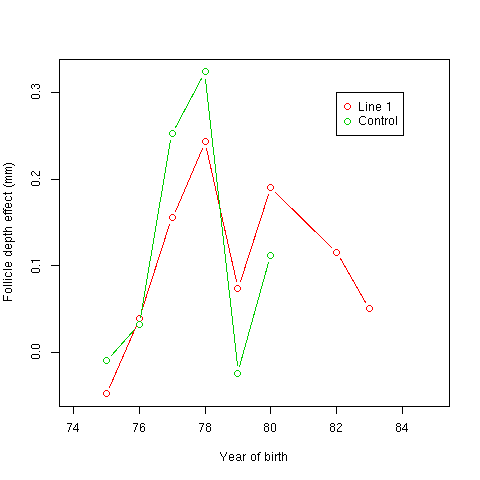
\includegraphics[width=0.9\textwidth]{dgl1.png}
%  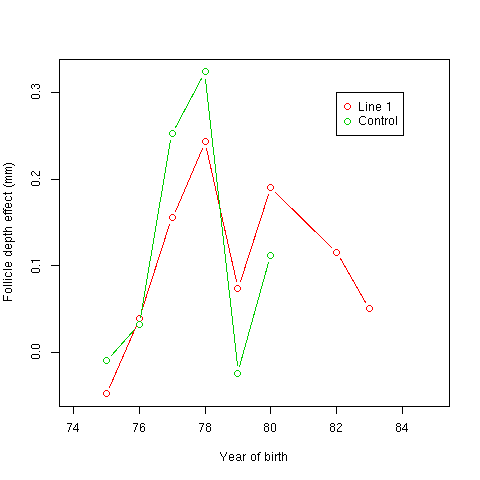
\includegraphics{dgl1.png}
  \caption{Direct response to selection for follicle depth in Line 1. Shifts in the difference between Line 1 and Control Line represent genetic change.}
  \label{fig:dgl1}
\end{figure}

%\end{document}



 Line 1 starts out with a smaller Fd than the Control Line, but changes from 1979 onward to having a larger Fd than the Control Line. There are a lot of data points missing. I am still waiting for CSIRO to complete the Fd measurements on Line 1 in 1984-85 and on the Control Line in 1981-85. Nevertheless we can conclude that there has been genetic change in Fd in Line 1 due to selection for Fd.

Figure~\ref{fig:dgl2} shows the direct response plot for Line 2 and the Control Line.

%\documentclass{article}
%\usepackage{graphicx,subfigure}
%\begin{document}

\begin{figure}[!htp]
  \centering
   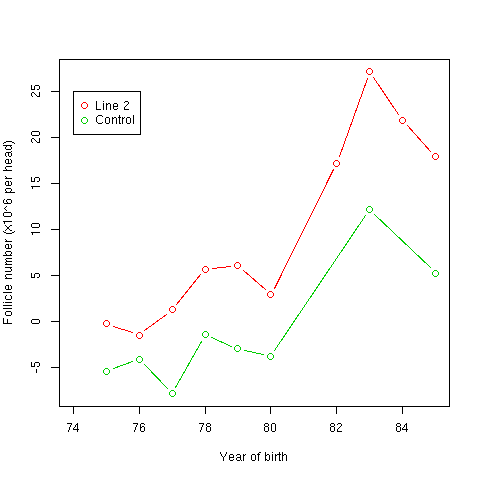
\includegraphics[width=0.9\textwidth]{dgl2.png}
%  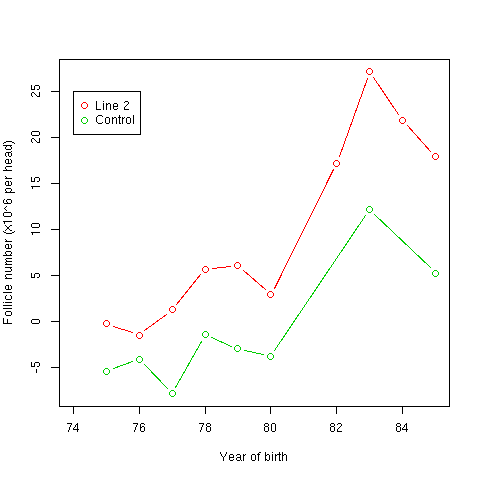
\includegraphics{dgl2.png}
  \caption{Direct response to selection for follicle number per head in Line 2. Shifts in the difference between Line 2 and Control Line represent genetic change.}
  \label{fig:dgl2}
\end{figure}

%\end{document}


Line 2 starts out with a larger number of follicles than the Control Line, and this difference increases with time. We can conclude that there has been genetic change in Fnt in Line 2 due to selection for Fnt. There is also a considerable environmental shift between years 80 and 82, both Line 2 and the Control Line have increased follicle numnber and this jump is manintained thereafter. The cause of this jump is unknown. It may be significant that there was a change of techniwue from manual counting to semi-automatic image processing in 1982.

Figure~\ref{fig:dgl3fd} shows the direct response plot for follicle depth for Line 3 and the Control Line. Figure~\ref{fig:dgl3fnt} shows the direct response plot for follicle number per head for Line 3 and the Control Line.

%\documentclass{article}
%\usepackage{graphicx,subfigure}
%\begin{document}

\begin{figure}[!htp]
  \centering
   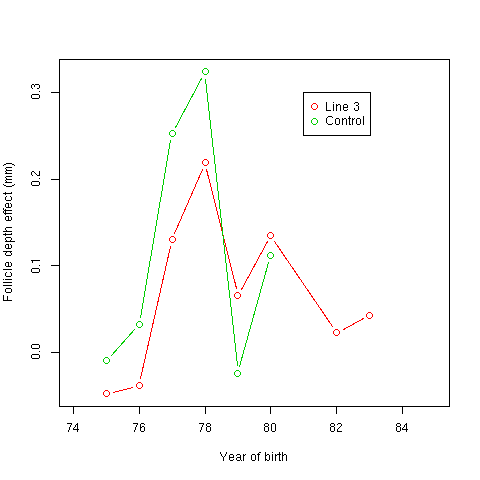
\includegraphics[width=0.9\textwidth]{dgl3fd.png}
%  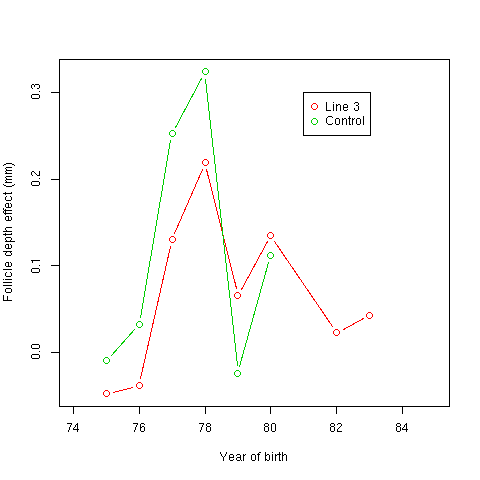
\includegraphics{dgl3fd.png}
  \caption{Direct response in follicle depth, to selection for follicle depth and follicle number per head in Line 3. Shifts in the difference between Line 3 and Control Line represent genetic change.}
  \label{fig:dgl3fd}
\end{figure}

%\end{document}


%\documentclass{article}
%\usepackage{graphicx,subfigure}
%\begin{document}

\begin{figure}[!htp]
  \centering
   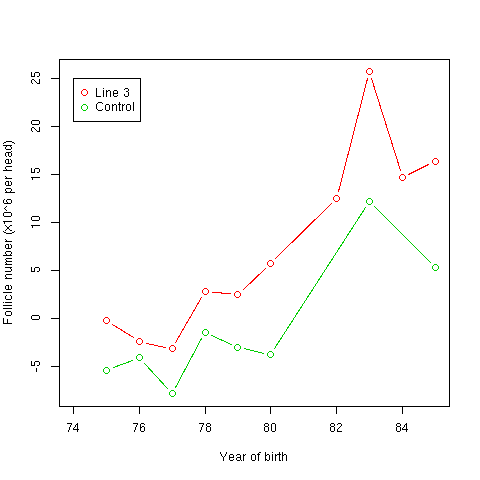
\includegraphics[width=0.9\textwidth]{dgl3fnt.png}
%  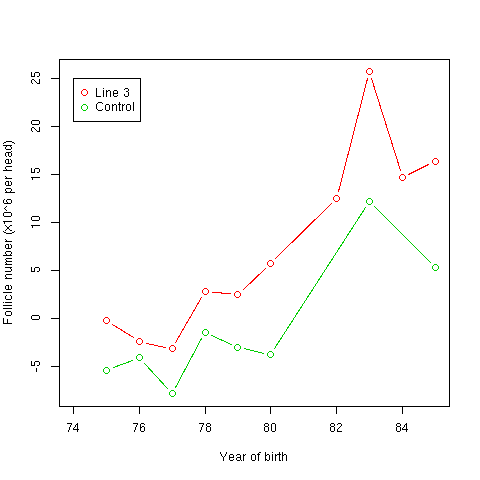
\includegraphics{dgl3fnt.png}
  \caption{Direct response in follicle number per head, to selection for follicle depth and follicle number per head in Line 3. Shifts in the difference between Line 3 and Control Line represent genetic change.}
  \label{fig:dgl3fnt}
\end{figure}

%\end{document}



Line 3 has achieved genetic change in both follicle depth and follicle number per head. The shift in follicle number between years 80 and 82 is again present. 

\subsection{Indirect responses to selection}
We will just look at indirect responses in clean wool weight, fibre diameter and staple length.

Figure~\ref{fig:dgcww} shows the indirect or correlated changes in clean wool weight ({\em Cwwadj}) in all three lines. There is no obvious change in clean wool weight in any of the three lines. There is a slight suggestion that the selected line might average out above the control line in both Line 2 and Line 3. This is not what was expected. The original thinking behind this experiment was that if one wanted to engineer a change in wool weight one had to put selection pressure on all of its components. The components of wool weight in this scenario were considred to be follicle size ( measured as follicle depth) and number of follicles ( measured as follicle number per head). It was expected that there would be a change in wool weight in Line 3 only. This did not occur. Possible explanations are
\begin{itemize}
\item the experiment did not continue for long enough
\item the two components ( follicle size and number) are in some way not an adequate representation of the biology of wool growth
\item the concept of components is somehow flawed
\end{itemize}

%\documentclass{article}
%\usepackage{graphicx,subfigure}
%\begin{document}

\begin{figure}[!htp]
  \centering
   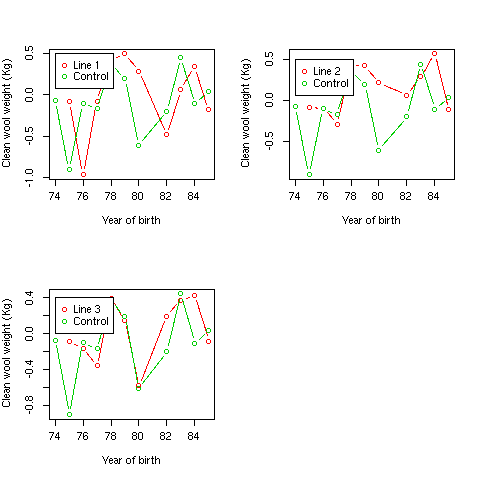
\includegraphics[width=0.9\textwidth]{dgcww.png}
%  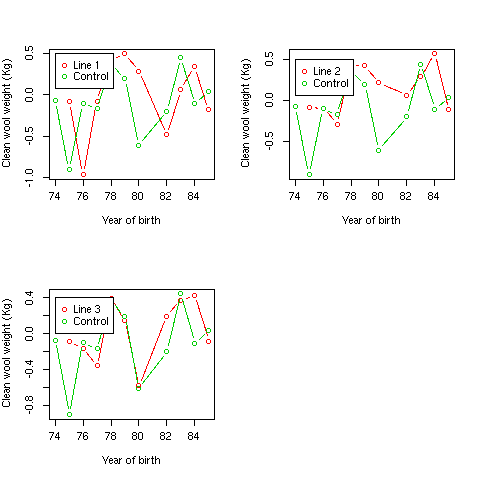
\includegraphics{dgcww.png}
  \caption{Indirect response in clean wool weight, to selection for follicle depth in Line 1, follicle number per head in Line 2, and follicle depth and follicle number per head in Line 3. Shifts in the difference between  each Line and the  Control Line represent genetic change.}
  \label{fig:dgcww}
\end{figure}

%\end{document}


We can look into this a little more thoroughly by seeing if there were any correlated changes in fibre diameter or in fibre length growth rate ( measured as staple length).

Figure~\ref{fig:dgdiam} and Figure~\ref{fig:dgstal} show the correlated changes in average fibre diameter and staple length.

%\documentclass{article}
%\usepackage{graphicx,subfigure}
%\begin{document}

\begin{figure}[!htp]
  \centering
   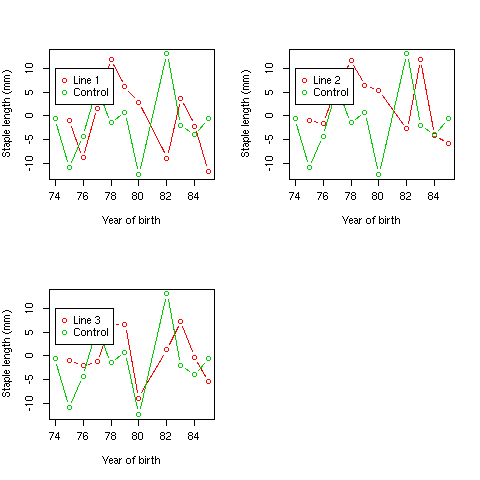
\includegraphics[width=0.9\textwidth]{dgstal.png}
%  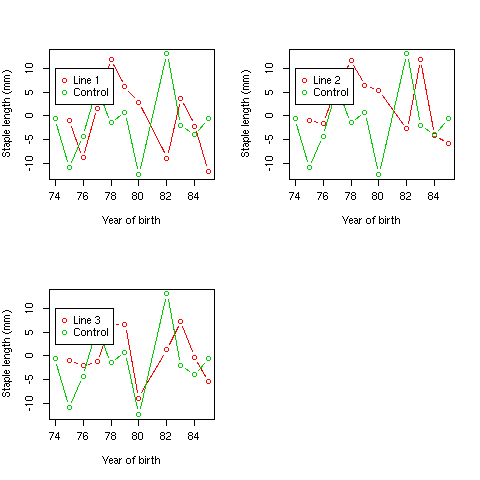
\includegraphics{dgstal.png}
  \caption{Indirect response in staple length, to selection for follicle depth in Line 1, follicle number per head in Line 2, and follicle depth and follicle number per head in Line 3. Shifts in the difference between  each Line and the  Control Line represent genetic change.}
  \label{fig:dgstal}
\end{figure}

%\end{document}


%\documentclass{article}
%\usepackage{graphicx,subfigure}
%\begin{document}

\begin{figure}[!htp]
  \centering
   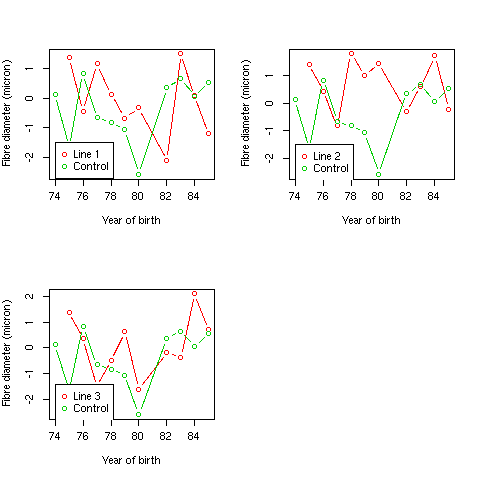
\includegraphics[width=0.9\textwidth]{dgdiam.png}
%  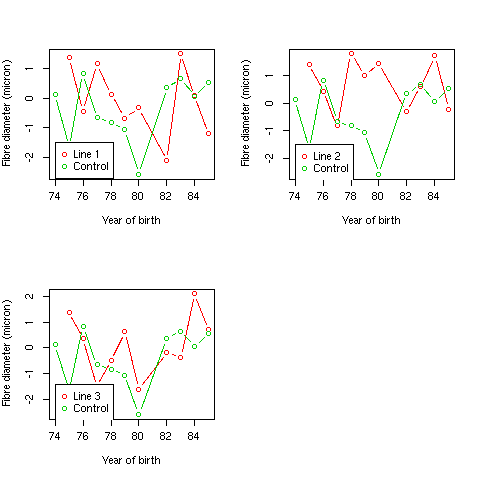
\includegraphics{dgdiam.png}
  \caption{Indirect response in fibre diameter, to selection for follicle depth in Line 1, follicle number per head in Line 2, and follicle depth and follicle number per head in Line 3. Shifts in the difference between  each Line and the  Control Line represent genetic change.}
  \label{fig:dgdiam}
\end{figure}

%\end{document}


There are no obvious correlated changes in staple length or fibre diameter in any of the 3 lines. There is a slight suggestion that staple length might average out higher than the Control line in Lines 2 and 3, as was observeed for clean wool weight. It is becoming clear that the experiment simply did not continue for enough years for correlated responses to be studied. Correlated genetic change is almost always smaller than direct responses to selection, and will therefore take more generations to detect. 

In view of the above, the experiment was simply not carried on for long enough to fulfil its original aim. The hypothesis that one can 'engineer' a genetic improvement in wool weight by changing its components in a coordinated way, is still open. A more detailed analysis of responses against amount of selection applied, is not warranted, and would be difficult to carry out because of the missing observations.

The experiment does however provide an important pedigreed data set with some interesting measurements not available elsewhere. We now proceed to an analysis of the pedigree data.

\subsection{Phenotypic parameters}
\subsubsection{Phenotypic variance}
\subsubsection{Phenotypic correlation}

\subsection{Genetic parameters}
\subsubsection{Proportion of variance which is genetic}
\subsubsection{Genetic correlation}

\subsection{Multivariate analysis}


\section{Discussion}

\section{Conclusions}

\begin{thebibliography}{99}

\bibitem{chap:65}
Chapman, R.E. (1965) The ovine arrector pili musculature and crimp formation 
    in wool. In "Biology of the Skin and Hair Growth" Angus and Robertson,
    Sydney, Ed. A.G. Lyne and B.F. Short. pp 201-232

\bibitem{hori:53}
Horio, M. and Kondo, T. (1953) Text. Res. J. 23:373

\bibitem{jack:75}
Jackson, N., Nay T. and Turner, Helen Newton (1975) Response to selection
    in Australian Merino sheep. VII Phenotypic and genetic parameters for
    some wool follicle characteristics and their correlation with wool and
    body traits. Aust. J. Agric. Res. 26:937-57

\bibitem{jack:15}
Jackson, N. and Watts, J.E. (2016) Staple crimp formation in the fleece of Merino sheep. 
Report available from the authors as a pdf document.

\bibitem{jack:16a}
Jackson, N.  and Watts J.E. (2016) Can we predict intrinsic fibre curvature from follicle curvature score? Report available from the author as a pdf document.

\bibitem{jack:15b}
Jackson, N. (2015) An Overview of the R package dmm.
    From http://cran.r-project.org/package=dmm
    Or https://github.com/cran/dmm

\bibitem{jack:86}
Jackson, N. Lax, J. and Wilson, R.L.(1986) Sex and selection for fleece weight in Merino sheep. Zeitschrift fur Tierzuchtung und Zuchtungsbiologie. Bd. 103:97-115

\bibitem{nago:81}
Nagorcka, B.N. (1981) Theoretical mechanism for crimp.
     Aust J. Biol. Sci. 34: 189-209

\bibitem{onio:62}
Onions, W.J. (1962) Wool: an introduction to its properties, varieties, uses
     and production. Ernest Benn limited, London, 1962

\bibitem{rend:78}
Rendel, J.M. and Nay, T. (1978) Selection for high and low ratio and high 
    and low primary density in Merino sheep. 
    Aust. J. Agric. Res. 29:1077-86

\bibitem{rprog:13}
R Core Team (2013). R: A language and environment for statistical
  computing. R Foundation for Statistical Computing, Vienna, Austria.
  ISBN 3-900051-07-0, URL http://www.R-project.org/.

\bibitem{sear:92}
Searle, S.R., Casella, G., and McCullock, C.E. (1992) Variance Components.
    John Wiley and Sons, New York.


\bibitem{swan:93}
Swan, P.G. (1993) Objective measurement of fibre crimp curvature and the bulk compressional properties of Australian wools. PhD Thesis, University of NSW, March 1993 

\bibitem{wats:77}
Watson, N., Jackson, N. and Whiteley, K.J. (1977) Inheritance of the resistance
    to compression property of Austrailian Merino wool and its genetic 
    correlation with follicle curvature and various wool and body 
    characters. Aust. J. Agric. Res. 28:1083-94

\bibitem{wola:14}
Wolak, M.E. (2014) nadiv: an R package to create relatedness matrices for
    estimating non-additive genetic variances in animal models.
    Methods in Ecology and Evolution 3:792-796.

\end{thebibliography}

%% latex table generated in R 3.2.4 by xtable 1.8-2 package
% Thu May 26 20:33:54 2016
\begin{table}[p]
\centering
\caption{Standard errors of fixed effects for Sex and Year-born-in-x-Line obtained from fitting model~\ref{model:fixed} for all 56 measured traits: Part 1/7.}
\label{tab:seb1}
\begin{tabular}{rrrrrrrrr}
  \hline
 & Stal & Diam & Bwt & WrN & WrB & WrT & Face & Gfw \\ 
  \hline
C(Sex, sum)1 & 0.16 & 0.02 & 0.07 & 0.01 & 0.01 & 0.02 & 0.02 & 0.01 \\ 
  C(YbxLi, sum)749 & 0.48 & 0.07 & 0.22 & 0.04 & 0.04 & 0.07 & 0.05 & 0.03 \\ 
  C(YbxLi, sum)750 & 1.16 & 0.17 & 0.53 & 0.09 & 0.10 & 0.18 & 0.13 & 0.06 \\ 
  C(YbxLi, sum)759 & 0.56 & 0.08 & 0.25 & 0.05 & 0.05 & 0.08 & 0.06 & 0.03 \\ 
  C(YbxLi, sum)761 & 1.29 & 0.19 & 0.59 & 0.10 & 0.11 & 0.20 & 0.14 & 0.07 \\ 
  C(YbxLi, sum)762 & 1.66 & 0.25 & 0.76 & 0.13 & 0.14 & 0.25 & 0.19 & 0.09 \\ 
  C(YbxLi, sum)763 & 1.32 & 0.20 & 0.60 & 0.11 & 0.11 & 0.20 & 0.15 & 0.07 \\ 
  C(YbxLi, sum)769 & 1.58 & 0.24 & 0.72 & 0.13 & 0.13 & 0.24 & 0.18 & 0.08 \\ 
  C(YbxLi, sum)771 & 1.18 & 0.18 & 0.54 & 0.10 & 0.10 & 0.18 & 0.13 & 0.06 \\ 
  C(YbxLi, sum)772 & 1.05 & 0.16 & 0.48 & 0.09 & 0.09 & 0.16 & 0.12 & 0.06 \\ 
  C(YbxLi, sum)773 & 1.00 & 0.15 & 0.45 & 0.08 & 0.08 & 0.15 & 0.11 & 0.05 \\ 
  C(YbxLi, sum)779 & 1.01 & 0.15 & 0.46 & 0.08 & 0.08 & 0.15 & 0.11 & 0.05 \\ 
  C(YbxLi, sum)781 & 1.02 & 0.15 & 0.47 & 0.08 & 0.09 & 0.15 & 0.11 & 0.05 \\ 
  C(YbxLi, sum)782 & 1.03 & 0.16 & 0.47 & 0.08 & 0.09 & 0.16 & 0.12 & 0.05 \\ 
  C(YbxLi, sum)783 & 1.08 & 0.16 & 0.49 & 0.09 & 0.09 & 0.16 & 0.12 & 0.06 \\ 
  C(YbxLi, sum)789 & 1.11 & 0.17 & 0.51 & 0.09 & 0.09 & 0.17 & 0.12 & 0.06 \\ 
  C(YbxLi, sum)791 & 1.14 & 0.17 & 0.52 & 0.09 & 0.10 & 0.17 & 0.13 & 0.06 \\ 
  C(YbxLi, sum)792 & 0.95 & 0.14 & 0.43 & 0.08 & 0.08 & 0.14 & 0.11 & 0.05 \\ 
  C(YbxLi, sum)793 & 0.91 & 0.14 & 0.42 & 0.07 & 0.08 & 0.14 & 0.10 & 0.05 \\ 
  C(YbxLi, sum)799 & 1.06 & 0.16 & 0.48 & 0.09 & 0.09 & 0.16 & 0.12 & 0.06 \\ 
  C(YbxLi, sum)801 & 1.04 & 0.16 & 0.47 & 0.08 & 0.09 & 0.16 & 0.12 & 0.06 \\ 
  C(YbxLi, sum)802 & 1.02 & 0.15 & 0.47 & 0.08 & 0.08 & 0.15 & 0.11 & 0.05 \\ 
  C(YbxLi, sum)803 & 0.96 & 0.15 & 0.44 & 0.08 & 0.08 & 0.15 & 0.11 & 0.05 \\ 
  C(YbxLi, sum)809 & 1.11 & 0.17 & 0.51 & 0.09 & 0.09 & 0.17 & 0.12 & 0.06 \\ 
  C(YbxLi, sum)821 & 0.98 & 0.15 & 0.45 & 0.08 & 0.08 & 0.15 & 0.11 & 0.05 \\ 
  C(YbxLi, sum)822 & 1.06 & 0.16 & 0.49 & 0.09 & 0.09 & 0.16 & 0.12 & 0.06 \\ 
  C(YbxLi, sum)823 & 1.04 & 0.16 & 0.48 & 0.08 & 0.09 & 0.16 & 0.12 & 0.06 \\ 
  C(YbxLi, sum)829 & 0.84 & 0.13 & 0.38 & 0.07 & 0.07 & 0.13 & 0.09 & 0.04 \\ 
  C(YbxLi, sum)831 & 0.99 & 0.15 & 0.45 & 0.08 & 0.08 & 0.15 & 0.11 & 0.05 \\ 
  C(YbxLi, sum)832 & 1.13 & 0.17 & 0.52 & 0.09 & 0.09 & 0.17 & 0.13 & 0.06 \\ 
  C(YbxLi, sum)833 & 0.97 & 0.15 & 0.44 & 0.08 & 0.08 & 0.15 & 0.11 & 0.05 \\ 
  C(YbxLi, sum)839 & 1.10 & 0.17 & 0.50 & 0.09 & 0.09 & 0.17 & 0.12 & 0.06 \\ 
  C(YbxLi, sum)841 & 1.02 & 0.15 & 0.47 & 0.08 & 0.09 & 0.16 & 0.11 & 0.05 \\ 
  C(YbxLi, sum)842 & 1.02 & 0.15 & 0.47 & 0.08 & 0.09 & 0.15 & 0.11 & 0.05 \\ 
  C(YbxLi, sum)843 & 0.91 & 0.14 & 0.42 & 0.07 & 0.08 & 0.14 & 0.10 & 0.05 \\ 
  C(YbxLi, sum)849 & 1.06 & 0.16 & 0.48 & 0.09 & 0.09 & 0.16 & 0.12 & 0.06 \\ 
  C(YbxLi, sum)851 & 1.01 & 0.15 & 0.46 & 0.08 & 0.08 & 0.15 & 0.11 & 0.05 \\ 
  C(YbxLi, sum)852 & 1.03 & 0.16 & 0.47 & 0.08 & 0.09 & 0.16 & 0.12 & 0.05 \\ 
  C(YbxLi, sum)853 & 0.97 & 0.15 & 0.44 & 0.08 & 0.08 & 0.15 & 0.11 & 0.05 \\ 
  C(YbxLi, sum)859 & 1.03 & 0.16 & 0.47 & 0.08 & 0.09 & 0.16 & 0.12 & 0.05 \\ 
  (Intercept) & 0.17 & 0.03 & 0.08 & 0.01 & 0.01 & 0.03 & 0.02 & 0.01 \\ 
   \hline
\end{tabular}
\end{table}

%% latex table generated in R 3.2.4 by xtable 1.8-2 package
% Thu May 26 20:34:18 2016
\begin{table}[p]
\centering
\caption{Standard errors of fixed effects for Sex and Year-born-in-x-Line obtained from fitting model~\ref{model:fixed} for all 56 measured traits: Part 2/7.}
\label{tab:seb2}
\begin{tabular}{rrrrrrrrr}
  \hline
 & Yld & Cww & Staladj & Gfwadj & Cwwadj & Crimp & Crwvl & Crst \\ 
  \hline
C(Sex, sum)1 & 0.08 & 0.01 & 0.19 & 0.01 & 0.01 & 0.05 & 0.01 & 0.16 \\ 
  C(YbxLi, sum)749 & 0.24 & 0.02 & 0.58 & 0.03 & 0.02 & 0.30 & 0.06 & 1.01 \\ 
  C(YbxLi, sum)750 & 0.58 & 0.04 & 1.39 & 0.07 & 0.05 & 0.17 & 0.03 & 0.56 \\ 
  C(YbxLi, sum)759 & 0.28 & 0.02 & 0.67 & 0.04 & 0.02 & 0.33 & 0.07 & 1.10 \\ 
  C(YbxLi, sum)761 & 0.64 & 0.05 & 1.54 & 0.08 & 0.06 & 0.42 & 0.08 & 1.41 \\ 
  C(YbxLi, sum)762 & 0.83 & 0.06 & 2.00 & 0.11 & 0.07 & 0.34 & 0.07 & 1.13 \\ 
  C(YbxLi, sum)763 & 0.66 & 0.05 & 1.58 & 0.08 & 0.06 & 0.40 & 0.08 & 1.33 \\ 
  C(YbxLi, sum)769 & 0.80 & 0.06 & 1.90 & 0.10 & 0.07 & 0.31 & 0.06 & 1.03 \\ 
  C(YbxLi, sum)771 & 0.59 & 0.04 & 1.42 & 0.08 & 0.05 & 0.28 & 0.06 & 0.93 \\ 
  C(YbxLi, sum)772 & 0.53 & 0.04 & 1.27 & 0.07 & 0.05 & 0.26 & 0.05 & 0.88 \\ 
  C(YbxLi, sum)773 & 0.50 & 0.04 & 1.19 & 0.06 & 0.04 & 0.27 & 0.05 & 0.90 \\ 
  C(YbxLi, sum)779 & 0.50 & 0.04 & 1.22 & 0.06 & 0.04 & 0.23 & 0.05 & 0.78 \\ 
  C(YbxLi, sum)781 & 0.51 & 0.04 & 1.23 & 0.07 & 0.04 &  &  &  \\ 
  C(YbxLi, sum)782 & 0.52 & 0.04 & 1.27 & 0.07 & 0.05 &  &  &  \\ 
  C(YbxLi, sum)783 & 0.54 & 0.04 & 1.33 & 0.07 & 0.05 &  &  &  \\ 
  C(YbxLi, sum)789 & 0.56 & 0.04 & 1.33 & 0.07 & 0.05 &  &  &  \\ 
  C(YbxLi, sum)791 & 0.57 & 0.04 & 1.39 & 0.07 & 0.05 &  &  &  \\ 
  C(YbxLi, sum)792 & 0.48 & 0.04 & 1.19 & 0.06 & 0.04 &  &  &  \\ 
  C(YbxLi, sum)793 & 0.46 & 0.03 & 1.10 & 0.06 & 0.04 &  &  &  \\ 
  C(YbxLi, sum)799 & 0.53 & 0.04 & 1.73 & 0.09 & 0.06 &  &  &  \\ 
  C(YbxLi, sum)801 & 0.52 & 0.04 & 1.25 & 0.07 & 0.05 &  &  &  \\ 
  C(YbxLi, sum)802 & 0.51 & 0.04 & 1.23 & 0.07 & 0.04 &  &  &  \\ 
  C(YbxLi, sum)803 & 0.48 & 0.04 & 1.17 & 0.06 & 0.04 &  &  &  \\ 
  C(YbxLi, sum)809 & 0.55 & 0.04 & 1.33 & 0.07 & 0.05 &  &  &  \\ 
  C(YbxLi, sum)821 & 0.49 & 0.04 & 1.18 & 0.06 & 0.04 &  &  &  \\ 
  C(YbxLi, sum)822 & 0.54 & 0.04 & 1.28 & 0.07 & 0.05 &  &  &  \\ 
  C(YbxLi, sum)823 & 0.52 & 0.04 & 1.26 & 0.07 & 0.05 &  &  &  \\ 
  C(YbxLi, sum)829 & 0.42 & 0.03 & 1.02 & 0.05 & 0.04 & 0.28 & 0.06 & 0.93 \\ 
  C(YbxLi, sum)831 & 0.50 & 0.04 & 1.20 & 0.06 & 0.04 &  &  &  \\ 
  C(YbxLi, sum)832 & 0.57 & 0.04 & 1.36 & 0.07 & 0.05 &  &  &  \\ 
  C(YbxLi, sum)833 & 0.48 & 0.04 & 1.16 & 0.06 & 0.04 &  &  &  \\ 
  C(YbxLi, sum)839 & 0.55 & 0.04 & 1.33 & 0.07 & 0.05 & 0.26 & 0.05 & 0.88 \\ 
  C(YbxLi, sum)841 & 0.52 & 0.04 & 1.23 & 0.07 & 0.04 & 0.25 & 0.05 & 0.82 \\ 
  C(YbxLi, sum)842 & 0.51 & 0.04 & 1.23 & 0.07 & 0.04 & 0.36 & 0.07 & 1.22 \\ 
  C(YbxLi, sum)843 & 0.45 & 0.03 & 1.09 & 0.06 & 0.04 & 0.27 & 0.05 & 0.91 \\ 
  C(YbxLi, sum)849 & 0.53 & 0.04 & 1.27 & 0.07 & 0.05 & 0.27 & 0.05 & 0.89 \\ 
  C(YbxLi, sum)851 & 0.51 & 0.04 & 1.22 & 0.06 & 0.04 & 0.26 & 0.05 & 0.87 \\ 
  C(YbxLi, sum)852 & 0.52 & 0.04 & 1.24 & 0.07 & 0.05 & 0.29 & 0.06 & 0.97 \\ 
  C(YbxLi, sum)853 & 0.49 & 0.04 & 1.17 & 0.06 & 0.04 & 0.26 & 0.05 & 0.87 \\ 
  C(YbxLi, sum)859 & 0.52 & 0.04 & 1.24 & 0.07 & 0.05 & 0.26 & 0.05 & 0.88 \\ 
  (Intercept) & 0.09 & 0.01 & 0.21 & 0.01 & 0.01 & 0.11 & 0.02 & 0.37 \\ 
   \hline
\end{tabular}
\end{table}

%% latex table generated in R 3.2.4 by xtable 1.8-2 package
% Thu May 26 20:34:35 2016
\begin{table}[p]
\centering
\caption{Standard errors of fixed effects for Sex and Year-born-in-x-Line obtained from fitting model~\ref{model:fixed} for all 56 measured traits: Part 3/7.}
\label{tab:seb3}
\begin{tabular}{rrrrrrrrr}
  \hline
 & Crstadj & Crwvt & Dp & Ds & Dps & DpovDs & CVDp & CVDs \\ 
  \hline
C(Sex, sum)1 & 0.19 & 0.00 & 0.14 & 0.08 & 0.08 & 0.01 & 0.19 & 0.11 \\ 
  C(YbxLi, sum)749 & 1.20 & 0.02 &  &  &  &  &  &  \\ 
  C(YbxLi, sum)750 & 0.68 & 0.01 &  &  &  &  &  &  \\ 
  C(YbxLi, sum)759 & 1.32 & 0.03 &  &  &  &  &  &  \\ 
  C(YbxLi, sum)761 & 1.68 & 0.03 &  &  &  &  &  &  \\ 
  C(YbxLi, sum)762 & 1.36 & 0.03 &  &  &  &  &  &  \\ 
  C(YbxLi, sum)763 & 1.59 & 0.03 &  &  &  &  &  &  \\ 
  C(YbxLi, sum)769 & 1.23 & 0.02 &  &  &  &  &  &  \\ 
  C(YbxLi, sum)771 & 1.12 & 0.02 &  &  &  &  &  &  \\ 
  C(YbxLi, sum)772 & 1.06 & 0.02 &  &  &  &  &  &  \\ 
  C(YbxLi, sum)773 & 1.08 & 0.02 &  &  &  &  &  &  \\ 
  C(YbxLi, sum)779 & 0.93 & 0.02 &  &  &  &  &  &  \\ 
  C(YbxLi, sum)781 &  &  &  &  &  &  &  &  \\ 
  C(YbxLi, sum)782 &  &  &  &  &  &  &  &  \\ 
  C(YbxLi, sum)783 &  &  &  &  &  &  &  &  \\ 
  C(YbxLi, sum)789 &  &  &  &  &  &  &  &  \\ 
  C(YbxLi, sum)791 &  &  &  &  &  &  &  &  \\ 
  C(YbxLi, sum)792 &  &  &  &  &  &  &  &  \\ 
  C(YbxLi, sum)793 &  &  &  &  &  &  &  &  \\ 
  C(YbxLi, sum)799 &  &  &  &  &  &  &  &  \\ 
  C(YbxLi, sum)801 &  &  &  &  &  &  &  &  \\ 
  C(YbxLi, sum)802 &  &  &  &  &  &  &  &  \\ 
  C(YbxLi, sum)803 &  &  &  &  &  &  &  &  \\ 
  C(YbxLi, sum)809 &  &  &  &  &  &  &  &  \\ 
  C(YbxLi, sum)821 &  &  &  &  &  &  &  &  \\ 
  C(YbxLi, sum)822 &  &  & 0.55 & 0.32 & 0.32 & 0.03 & 0.73 & 0.44 \\ 
  C(YbxLi, sum)823 &  &  & 0.56 & 0.33 & 0.33 & 0.03 & 0.75 & 0.45 \\ 
  C(YbxLi, sum)829 & 1.12 & 0.02 &  &  &  &  &  &  \\ 
  C(YbxLi, sum)831 &  &  & 0.65 & 0.39 & 0.38 & 0.03 & 0.87 & 0.52 \\ 
  C(YbxLi, sum)832 &  &  & 0.72 & 0.42 & 0.42 & 0.03 & 0.96 & 0.57 \\ 
  C(YbxLi, sum)833 &  &  & 0.68 & 0.40 & 0.40 & 0.03 & 0.91 & 0.55 \\ 
  C(YbxLi, sum)839 & 1.05 & 0.02 & 0.66 & 0.39 & 0.38 & 0.03 & 0.88 & 0.52 \\ 
  C(YbxLi, sum)841 & 0.98 & 0.02 & 0.71 & 0.42 & 0.42 & 0.03 & 0.95 & 0.57 \\ 
  C(YbxLi, sum)842 & 1.46 & 0.03 & 0.73 & 0.43 & 0.42 & 0.03 & 0.97 & 0.58 \\ 
  C(YbxLi, sum)843 & 1.09 & 0.02 & 0.61 & 0.36 & 0.36 & 0.03 & 0.82 & 0.49 \\ 
  C(YbxLi, sum)849 & 1.07 & 0.02 &  &  &  &  &  &  \\ 
  C(YbxLi, sum)851 & 1.04 & 0.02 & 0.55 & 0.32 & 0.32 & 0.03 & 0.73 & 0.44 \\ 
  C(YbxLi, sum)852 & 1.16 & 0.02 & 0.58 & 0.34 & 0.34 & 0.03 & 0.78 & 0.47 \\ 
  C(YbxLi, sum)853 & 1.04 & 0.02 & 0.55 & 0.32 & 0.32 & 0.03 & 0.73 & 0.44 \\ 
  C(YbxLi, sum)859 & 1.05 & 0.02 & 0.65 & 0.38 & 0.38 & 0.03 & 0.87 & 0.52 \\ 
  (Intercept) & 0.44 & 0.01 & 0.42 & 0.25 & 0.24 & 0.02 & 0.56 & 0.33 \\ 
   \hline
\end{tabular}
\end{table}

%% latex table generated in R 3.2.4 by xtable 1.8-2 package
% Thu May 26 20:34:54 2016
\begin{table}[p]
\centering
\caption{Standard errors of fixed effects for Sex and Year-born-in-x-Line obtained from fitting model~\ref{model:fixed} for all 56 measured traits: Part 4/7.}
\label{tab:seb4}
\begin{tabular}{rrrrrrrrr}
  \hline
 & MaxDp & MinDp & MaxDs & MinDs & SDDp & SDDs & SDD & CVD \\ 
  \hline
C(Sex, sum)1 & 0.27 & 0.15 & 0.21 & 0.10 & 0.06 & 0.02 & 0.02 & 0.11 \\ 
  C(YbxLi, sum)749 &  &  &  &  &  &  &  &  \\ 
  C(YbxLi, sum)750 &  &  &  &  &  &  &  &  \\ 
  C(YbxLi, sum)759 &  &  &  &  &  &  &  &  \\ 
  C(YbxLi, sum)761 &  &  &  &  &  &  &  &  \\ 
  C(YbxLi, sum)762 &  &  &  &  &  &  &  &  \\ 
  C(YbxLi, sum)763 &  &  &  &  &  &  &  &  \\ 
  C(YbxLi, sum)769 &  &  &  &  &  &  &  &  \\ 
  C(YbxLi, sum)771 &  &  &  &  &  &  &  &  \\ 
  C(YbxLi, sum)772 &  &  &  &  &  &  &  &  \\ 
  C(YbxLi, sum)773 &  &  &  &  &  &  &  &  \\ 
  C(YbxLi, sum)779 &  &  &  &  &  &  &  &  \\ 
  C(YbxLi, sum)781 &  &  &  &  &  &  &  &  \\ 
  C(YbxLi, sum)782 &  &  &  &  &  &  &  &  \\ 
  C(YbxLi, sum)783 &  &  &  &  &  &  &  &  \\ 
  C(YbxLi, sum)789 &  &  &  &  &  &  &  &  \\ 
  C(YbxLi, sum)791 &  &  &  &  &  &  &  &  \\ 
  C(YbxLi, sum)792 &  &  &  &  &  &  &  &  \\ 
  C(YbxLi, sum)793 &  &  &  &  &  &  &  &  \\ 
  C(YbxLi, sum)799 &  &  &  &  &  &  &  &  \\ 
  C(YbxLi, sum)801 &  &  &  &  &  &  &  &  \\ 
  C(YbxLi, sum)802 &  &  &  &  &  &  &  &  \\ 
  C(YbxLi, sum)803 &  &  &  &  &  &  &  &  \\ 
  C(YbxLi, sum)809 &  &  &  &  &  &  &  &  \\ 
  C(YbxLi, sum)821 &  &  &  &  &  &  &  &  \\ 
  C(YbxLi, sum)822 & 1.07 & 0.58 & 0.83 & 0.39 & 0.22 & 0.09 & 0.09 & 0.43 \\ 
  C(YbxLi, sum)823 & 1.09 & 0.59 & 0.85 & 0.40 & 0.23 & 0.09 & 0.10 & 0.44 \\ 
  C(YbxLi, sum)829 &  &  &  &  &  &  &  &  \\ 
  C(YbxLi, sum)831 & 1.28 & 0.69 & 0.99 & 0.47 & 0.27 & 0.11 & 0.11 & 0.51 \\ 
  C(YbxLi, sum)832 & 1.41 & 0.76 & 1.09 & 0.51 & 0.29 & 0.12 & 0.12 & 0.56 \\ 
  C(YbxLi, sum)833 & 1.34 & 0.72 & 1.03 & 0.49 & 0.28 & 0.12 & 0.12 & 0.54 \\ 
  C(YbxLi, sum)839 & 1.28 & 0.69 & 0.99 & 0.47 & 0.27 & 0.11 & 0.11 & 0.52 \\ 
  C(YbxLi, sum)841 & 1.39 & 0.75 & 1.08 & 0.51 & 0.29 & 0.12 & 0.12 & 0.56 \\ 
  C(YbxLi, sum)842 & 1.42 & 0.77 & 1.10 & 0.52 & 0.29 & 0.12 & 0.12 & 0.57 \\ 
  C(YbxLi, sum)843 & 1.20 & 0.65 & 0.93 & 0.44 & 0.25 & 0.10 & 0.10 & 0.48 \\ 
  C(YbxLi, sum)849 &  &  &  &  &  &  &  &  \\ 
  C(YbxLi, sum)851 & 1.07 & 0.58 & 0.83 & 0.39 & 0.22 & 0.09 & 0.09 & 0.43 \\ 
  C(YbxLi, sum)852 & 1.14 & 0.62 & 0.88 & 0.42 & 0.24 & 0.10 & 0.10 & 0.46 \\ 
  C(YbxLi, sum)853 & 1.07 & 0.58 & 0.83 & 0.39 & 0.22 & 0.09 & 0.09 & 0.43 \\ 
  C(YbxLi, sum)859 & 1.28 & 0.69 & 0.99 & 0.47 & 0.27 & 0.11 & 0.11 & 0.51 \\ 
  (Intercept) & 0.81 & 0.44 & 0.63 & 0.30 & 0.17 & 0.07 & 0.07 & 0.33 \\ 
   \hline
\end{tabular}
\end{table}

%% latex table generated in R 3.2.4 by xtable 1.8-2 package
% Thu May 26 20:35:12 2016
\begin{table}[p]
\centering
\caption{Standard errors of fixed effects for Sex and Year-born-in-x-Line obtained from fitting model~\ref{model:fixed} for all 56 measured traits: Part 5/7.}
\label{tab:seb5}
\begin{tabular}{rrrrrrrrr}
  \hline
 & Gt30Dp & Gt30Ds & Gt30D & Fnua & Fr & Fnt & Sarea & Fd \\ 
  \hline
C(Sex, sum)1 & 0.68 & 0.11 & 0.13 & 0.23 & 0.07 & 0.23 & 0.00 & 0.00 \\ 
  C(YbxLi, sum)749 &  &  &  &  &  &  &  &  \\ 
  C(YbxLi, sum)750 &  &  &  & 0.93 & 0.29 & 0.91 & 0.01 & 0.01 \\ 
  C(YbxLi, sum)759 &  &  &  & 2.20 & 0.70 & 2.16 & 0.01 & 0.03 \\ 
  C(YbxLi, sum)761 &  &  &  & 2.32 & 0.74 & 2.28 & 0.02 & 0.03 \\ 
  C(YbxLi, sum)762 &  &  &  & 1.85 & 0.59 & 1.81 & 0.01 & 0.02 \\ 
  C(YbxLi, sum)763 &  &  &  & 2.19 & 0.70 & 2.15 & 0.01 & 0.03 \\ 
  C(YbxLi, sum)769 &  &  &  & 1.67 & 0.53 & 1.64 & 0.01 & 0.02 \\ 
  C(YbxLi, sum)771 &  &  &  & 1.51 & 0.48 & 1.48 & 0.01 & 0.02 \\ 
  C(YbxLi, sum)772 &  &  &  & 1.46 & 0.46 & 1.43 & 0.01 & 0.02 \\ 
  C(YbxLi, sum)773 &  &  &  & 1.46 & 0.46 & 1.43 & 0.01 & 0.02 \\ 
  C(YbxLi, sum)779 &  &  &  & 1.26 & 0.40 & 1.24 & 0.01 & 0.02 \\ 
  C(YbxLi, sum)781 &  &  &  & 1.58 & 0.50 & 1.55 & 0.01 & 0.02 \\ 
  C(YbxLi, sum)782 &  &  &  & 1.48 & 0.47 & 1.45 & 0.01 & 0.02 \\ 
  C(YbxLi, sum)783 &  &  &  & 1.48 & 0.47 & 1.45 & 0.01 & 0.02 \\ 
  C(YbxLi, sum)789 &  &  &  & 1.36 & 0.43 & 1.34 & 0.01 & 0.02 \\ 
  C(YbxLi, sum)791 &  &  &  & 1.53 & 0.48 & 1.50 & 0.01 & 0.02 \\ 
  C(YbxLi, sum)792 &  &  &  & 1.47 & 0.47 & 1.44 & 0.01 & 0.02 \\ 
  C(YbxLi, sum)793 &  &  &  & 1.49 & 0.47 & 1.46 & 0.01 & 0.02 \\ 
  C(YbxLi, sum)799 &  &  &  & 1.41 & 0.45 & 1.38 & 0.01 & 0.02 \\ 
  C(YbxLi, sum)801 &  &  &  & 1.49 & 0.47 & 1.46 & 0.01 & 0.02 \\ 
  C(YbxLi, sum)802 &  &  &  & 1.53 & 0.48 & 1.50 & 0.01 & 0.02 \\ 
  C(YbxLi, sum)803 &  &  &  & 1.49 & 0.47 & 1.46 & 0.01 & 0.02 \\ 
  C(YbxLi, sum)809 &  &  &  & 1.43 & 0.45 & 1.40 & 0.01 & 0.02 \\ 
  C(YbxLi, sum)821 &  &  &  & 1.61 & 0.51 & 1.59 & 0.01 & 0.02 \\ 
  C(YbxLi, sum)822 & 2.66 & 0.45 & 0.49 & 1.41 & 0.45 & 1.39 & 0.01 & 0.02 \\ 
  C(YbxLi, sum)823 & 2.72 & 0.46 & 0.50 & 1.47 & 0.47 & 1.45 & 0.01 & 0.02 \\ 
  C(YbxLi, sum)829 &  &  &  &  &  &  &  &  \\ 
  C(YbxLi, sum)831 & 3.19 & 0.54 & 0.59 & 1.89 & 0.60 & 1.85 & 0.01 & 0.03 \\ 
  C(YbxLi, sum)832 & 3.50 & 0.59 & 0.65 & 2.14 & 0.68 & 2.10 & 0.01 & 0.03 \\ 
  C(YbxLi, sum)833 & 3.33 & 0.56 & 0.62 & 2.03 & 0.64 & 1.99 & 0.01 & 0.03 \\ 
  C(YbxLi, sum)839 & 3.20 & 0.54 & 0.59 & 1.88 & 0.60 & 1.84 & 0.01 &  \\ 
  C(YbxLi, sum)841 & 3.47 & 0.59 & 0.64 & 1.88 & 0.60 & 1.84 & 0.01 &  \\ 
  C(YbxLi, sum)842 & 3.53 & 0.60 & 0.65 & 2.02 & 0.64 & 1.98 & 0.01 &  \\ 
  C(YbxLi, sum)843 & 2.99 & 0.51 & 0.55 & 1.70 & 0.54 & 1.67 & 0.01 &  \\ 
  C(YbxLi, sum)849 &  &  &  &  &  &  &  &  \\ 
  C(YbxLi, sum)851 & 2.66 & 0.45 & 0.49 & 1.40 & 0.44 & 1.38 & 0.01 &  \\ 
  C(YbxLi, sum)852 & 2.84 & 0.48 & 0.52 & 1.59 & 0.51 & 1.57 & 0.01 &  \\ 
  C(YbxLi, sum)853 & 2.68 & 0.45 & 0.49 & 1.43 & 0.45 & 1.40 & 0.01 &  \\ 
  C(YbxLi, sum)859 & 3.18 & 0.54 & 0.59 & 1.86 & 0.59 & 1.83 & 0.01 &  \\ 
  (Intercept) & 2.03 & 0.34 & 0.38 & 0.59 & 0.19 & 0.58 & 0.00 & 0.01 \\ 
   \hline
\end{tabular}
\end{table}

%% latex table generated in R 3.2.4 by xtable 1.8-2 package
% Thu May 26 20:35:38 2016
\begin{table}[p]
\centering
\caption{Standard errors of fixed effects for Sex and Year-born-in-x-Line obtained from fitting model~\ref{model:fixed} for all 56 measured traits: Part 6/7.}
\label{tab:seb6}
\begin{tabular}{rrrrrrrrr}
  \hline
 & Fc & Fu & Colour & Fly & Flcrot & Bactst & MycD & Bcts \\ 
  \hline
C(Sex, sum)1 & 0.02 & 0.02 & 0.01 & 0.02 & 0.03 & 0.01 & 0.02 & 0.03 \\ 
  C(YbxLi, sum)749 &  &  & 0.10 & 0.18 & 0.24 &  &  &  \\ 
  C(YbxLi, sum)750 & 0.08 & 0.06 & 0.06 & 0.10 & 0.13 &  &  &  \\ 
  C(YbxLi, sum)759 & 0.20 & 0.14 & 0.11 & 0.20 & 0.26 &  &  & 0.21 \\ 
  C(YbxLi, sum)761 & 0.21 & 0.15 & 0.15 & 0.26 & 0.33 &  &  & 0.27 \\ 
  C(YbxLi, sum)762 & 0.17 & 0.12 & 0.12 & 0.21 & 0.27 &  &  & 0.22 \\ 
  C(YbxLi, sum)763 & 0.20 & 0.14 & 0.14 & 0.25 & 0.32 &  &  & 0.26 \\ 
  C(YbxLi, sum)769 & 0.15 & 0.11 & 0.11 & 0.19 & 0.24 &  &  & 0.20 \\ 
  C(YbxLi, sum)771 & 0.14 & 0.10 &  &  &  &  &  & 0.18 \\ 
  C(YbxLi, sum)772 & 0.13 & 0.10 &  &  &  &  &  & 0.18 \\ 
  C(YbxLi, sum)773 & 0.13 & 0.10 &  &  &  &  &  & 0.18 \\ 
  C(YbxLi, sum)779 & 0.11 & 0.08 & 0.08 & 0.14 & 0.18 &  &  & 0.15 \\ 
  C(YbxLi, sum)781 & 0.14 & 0.10 & 0.10 & 0.18 & 0.23 &  &  & 0.19 \\ 
  C(YbxLi, sum)782 & 0.13 & 0.10 & 0.09 & 0.17 & 0.21 & 0.06 & 0.12 & 0.18 \\ 
  C(YbxLi, sum)783 & 0.13 & 0.10 & 0.09 & 0.16 & 0.21 & 0.06 & 0.12 & 0.18 \\ 
  C(YbxLi, sum)789 & 0.12 & 0.09 & 0.08 & 0.15 & 0.19 & 0.05 & 0.11 & 0.16 \\ 
  C(YbxLi, sum)791 & 0.14 & 0.10 & 0.10 & 0.17 & 0.22 & 0.06 & 0.12 & 0.18 \\ 
  C(YbxLi, sum)792 & 0.13 & 0.10 & 0.09 & 0.16 & 0.21 & 0.06 & 0.12 & 0.18 \\ 
  C(YbxLi, sum)793 & 0.13 & 0.10 & 0.09 & 0.17 & 0.21 & 0.06 & 0.12 & 0.18 \\ 
  C(YbxLi, sum)799 & 0.13 & 0.09 & 0.09 & 0.16 & 0.20 & 0.05 & 0.12 & 0.17 \\ 
  C(YbxLi, sum)801 & 0.13 & 0.10 & 0.09 & 0.17 & 0.21 & 0.06 & 0.12 & 0.18 \\ 
  C(YbxLi, sum)802 & 0.14 & 0.10 & 0.10 & 0.17 & 0.22 & 0.06 & 0.12 & 0.18 \\ 
  C(YbxLi, sum)803 & 0.13 & 0.10 & 0.09 & 0.17 & 0.21 & 0.06 & 0.12 & 0.18 \\ 
  C(YbxLi, sum)809 & 0.13 & 0.09 & 0.09 & 0.16 & 0.21 & 0.05 & 0.12 & 0.17 \\ 
  C(YbxLi, sum)821 & 0.15 & 0.11 & 0.10 & 0.18 & 0.23 & 0.06 & 0.13 & 0.19 \\ 
  C(YbxLi, sum)822 & 0.13 & 0.09 & 0.09 & 0.16 & 0.20 & 0.05 & 0.12 & 0.17 \\ 
  C(YbxLi, sum)823 & 0.13 & 0.10 & 0.09 & 0.16 & 0.21 & 0.06 & 0.12 & 0.18 \\ 
  C(YbxLi, sum)829 &  &  & 0.09 & 0.17 & 0.21 & 0.06 & 0.12 & 0.18 \\ 
  C(YbxLi, sum)831 & 0.19 & 0.14 & 0.10 & 0.17 & 0.22 & 0.06 & 0.12 & 0.19 \\ 
  C(YbxLi, sum)832 & 0.19 & 0.14 & 0.10 & 0.18 & 0.23 & 0.06 & 0.13 & 0.19 \\ 
  C(YbxLi, sum)833 & 0.22 & 0.16 & 0.10 & 0.18 & 0.23 & 0.06 & 0.13 & 0.20 \\ 
  C(YbxLi, sum)839 &  &  & 0.09 & 0.15 & 0.20 & 0.05 & 0.12 & 0.17 \\ 
  C(YbxLi, sum)841 &  &  & 0.09 & 0.15 & 0.19 & 0.05 & 0.11 & 0.16 \\ 
  C(YbxLi, sum)842 &  &  & 0.10 & 0.17 & 0.22 & 0.06 & 0.12 & 0.18 \\ 
  C(YbxLi, sum)843 &  &  & 0.09 & 0.17 & 0.21 & 0.06 & 0.12 & 0.18 \\ 
  C(YbxLi, sum)849 &  &  & 0.09 & 0.16 & 0.21 & 0.06 & 0.12 & 0.18 \\ 
  C(YbxLi, sum)851 &  &  & 0.09 & 0.16 & 0.20 & 0.05 & 0.12 & 0.17 \\ 
  C(YbxLi, sum)852 &  &  & 0.10 & 0.18 & 0.23 & 0.06 & 0.13 & 0.19 \\ 
  C(YbxLi, sum)853 &  &  & 0.09 & 0.16 & 0.20 & 0.05 & 0.12 & 0.17 \\ 
  C(YbxLi, sum)859 &  &  & 0.09 & 0.16 & 0.20 & 0.05 & 0.12 & 0.17 \\ 
  (Intercept) & 0.05 & 0.04 & 0.04 & 0.07 & 0.09 & 0.04 & 0.09 & 0.08 \\ 
   \hline
\end{tabular}
\end{table}

%% latex table generated in R 3.2.4 by xtable 1.8-2 package
% Thu May 26 20:35:54 2016
\begin{table}[p]
\centering
\caption{Standard errors of fixed effects for Sex and Year-born-in-x-Line obtained from fitting model~\ref{model:fixed} for all 56 measured traits: Part 7/7.}
\label{tab:seb7}
\begin{tabular}{rrrrrrrrr}
  \hline
 & Bctb & Weanwt & NLB & NLW & Fnpua & Fnsua & Fnpt & Fnst \\ 
  \hline
C(Sex, sum)1 & 0.03 & 0.05 & 0.01 & 0.01 & 0.01 & 0.23 & 0.01 & 0.22 \\ 
  C(YbxLi, sum)749 &  &  & 0.02 & 0.02 &  &  &  &  \\ 
  C(YbxLi, sum)750 &  &  & 0.06 & 0.05 & 0.05 & 0.91 & 0.05 & 0.89 \\ 
  C(YbxLi, sum)759 & 0.22 & 0.44 & 0.03 & 0.02 & 0.11 & 2.15 & 0.11 & 2.11 \\ 
  C(YbxLi, sum)761 & 0.28 & 0.56 & 0.06 & 0.06 & 0.12 & 2.27 & 0.12 & 2.23 \\ 
  C(YbxLi, sum)762 & 0.23 & 0.46 & 0.08 & 0.07 & 0.10 & 1.80 & 0.09 & 1.77 \\ 
  C(YbxLi, sum)763 & 0.27 & 0.53 & 0.06 & 0.06 & 0.11 & 2.14 & 0.11 & 2.10 \\ 
  C(YbxLi, sum)769 & 0.21 & 0.42 & 0.08 & 0.07 & 0.09 & 1.63 & 0.09 & 1.60 \\ 
  C(YbxLi, sum)771 & 0.19 & 0.38 & 0.06 & 0.05 & 0.08 & 1.48 & 0.08 & 1.45 \\ 
  C(YbxLi, sum)772 & 0.18 & 0.36 & 0.05 & 0.05 & 0.08 & 1.42 & 0.07 & 1.40 \\ 
  C(YbxLi, sum)773 & 0.18 & 0.37 & 0.05 & 0.04 & 0.08 & 1.42 & 0.07 & 1.40 \\ 
  C(YbxLi, sum)779 & 0.16 & 0.32 & 0.05 & 0.04 & 0.06 & 1.23 & 0.06 & 1.21 \\ 
  C(YbxLi, sum)781 & 0.20 & 0.39 & 0.05 & 0.05 & 0.08 & 1.55 & 0.08 & 1.52 \\ 
  C(YbxLi, sum)782 & 0.19 & 0.37 & 0.05 & 0.05 & 0.08 & 1.44 & 0.08 & 1.42 \\ 
  C(YbxLi, sum)783 & 0.19 & 0.37 & 0.05 & 0.05 & 0.08 & 1.44 & 0.08 & 1.42 \\ 
  C(YbxLi, sum)789 & 0.17 & 0.33 & 0.05 & 0.05 & 0.07 & 1.33 & 0.07 & 1.31 \\ 
  C(YbxLi, sum)791 & 0.19 & 0.38 & 0.06 & 0.05 & 0.08 & 1.49 & 0.08 & 1.47 \\ 
  C(YbxLi, sum)792 & 0.18 & 0.37 & 0.05 & 0.04 & 0.08 & 1.44 & 0.07 & 1.41 \\ 
  C(YbxLi, sum)793 & 0.19 & 0.37 & 0.04 & 0.04 & 0.08 & 1.45 & 0.08 & 1.43 \\ 
  C(YbxLi, sum)799 & 0.18 & 0.36 & 0.05 & 0.05 & 0.07 & 1.38 & 0.07 & 1.35 \\ 
  C(YbxLi, sum)801 & 0.19 & 0.37 & 0.05 & 0.05 & 0.08 & 1.45 & 0.08 & 1.43 \\ 
  C(YbxLi, sum)802 & 0.19 & 0.38 & 0.05 & 0.04 & 0.08 & 1.49 & 0.08 & 1.47 \\ 
  C(YbxLi, sum)803 & 0.19 & 0.37 & 0.05 & 0.04 & 0.08 & 1.45 & 0.08 & 1.43 \\ 
  C(YbxLi, sum)809 & 0.18 & 0.36 & 0.05 & 0.05 & 0.07 & 1.40 & 0.07 & 1.37 \\ 
  C(YbxLi, sum)821 & 0.20 & 0.40 & 0.05 & 0.04 & 0.08 & 1.58 & 0.08 & 1.55 \\ 
  C(YbxLi, sum)822 & 0.18 & 0.35 & 0.05 & 0.05 & 0.07 & 1.38 & 0.07 & 1.36 \\ 
  C(YbxLi, sum)823 & 0.18 & 0.37 & 0.05 & 0.05 & 0.08 & 1.44 & 0.07 & 1.41 \\ 
  C(YbxLi, sum)829 & 0.19 & 0.37 & 0.04 & 0.04 &  &  &  &  \\ 
  C(YbxLi, sum)831 & 0.19 & 0.39 & 0.05 & 0.04 & 0.10 & 1.84 & 0.10 & 1.81 \\ 
  C(YbxLi, sum)832 & 0.20 & 0.40 & 0.06 & 0.05 & 0.11 & 2.09 & 0.11 & 2.06 \\ 
  C(YbxLi, sum)833 & 0.20 & 0.41 & 0.05 & 0.04 & 0.10 & 1.98 & 0.10 & 1.95 \\ 
  C(YbxLi, sum)839 & 0.17 & 0.35 & 0.05 & 0.05 & 0.10 & 1.83 & 0.10 & 1.80 \\ 
  C(YbxLi, sum)841 & 0.17 & 0.34 & 0.05 & 0.05 & 0.10 & 1.83 & 0.10 & 1.80 \\ 
  C(YbxLi, sum)842 & 0.19 & 0.38 & 0.05 & 0.05 & 0.10 & 1.97 & 0.10 & 1.94 \\ 
  C(YbxLi, sum)843 & 0.19 & 0.37 & 0.04 & 0.04 & 0.09 & 1.66 & 0.09 & 1.63 \\ 
  C(YbxLi, sum)849 & 0.18 & 0.37 & 0.05 & 0.05 &  &  &  &  \\ 
  C(YbxLi, sum)851 & 0.18 & 0.35 & 0.05 & 0.04 & 0.07 & 1.37 & 0.07 & 1.34 \\ 
  C(YbxLi, sum)852 & 0.20 & 0.39 & 0.05 & 0.05 & 0.08 & 1.56 & 0.08 & 1.53 \\ 
  C(YbxLi, sum)853 & 0.18 & 0.36 & 0.05 & 0.04 & 0.07 & 1.39 & 0.07 & 1.37 \\ 
  C(YbxLi, sum)859 & 0.18 & 0.35 & 0.05 & 0.05 & 0.10 & 1.82 & 0.09 & 1.78 \\ 
  (Intercept) & 0.09 & 0.17 & 0.01 & 0.01 & 0.03 & 0.58 & 0.03 & 0.57 \\ 
   \hline
\end{tabular}
\end{table}


\end{document}

